\documentclass[12pt,
bibtotoc,liststotoc,appendixprefix,
twoside=off,paper=a4,headings=small]{scrbook}
%
% Packages
% -----------------------------------
\usepackage[
  paper=a4paper,
  left=12.5mm,
  right=25mm,
  top=25mm,
  bottom=50mm,
  bindingoffset=10mm]{geometry}		% Seitenränder und Bindungskorrektur einstellen

\usepackage{amsmath,amssymb,amsfonts}
\usepackage{algorithmic}            
\usepackage{apacite} 				% Literatur-Referenzen: American Psycholog. Assoc.
\usepackage{natbib}	
\usepackage[style=iso]{datetime2}
\setcitestyle{round,aysep={}} 		% Indizierg. in runden Klammern, zw. Autor u. Jahr
%\usepackage[latin1]{inputenc} 		% Umlaute im Text
\usepackage[english]{babel}			% Rechtschreibg.
\usepackage[T1]{fontenc}
\usepackage{lmodern}				% Schriftfamilie
\usepackage{microtype}				% für die Mikrotypografie (besseres Schriftbild)
\usepackage{comment}
\usepackage{graphicx} 				% Grafiken einfügen (pdf,png - aber jpg vermeiden)
\graphicspath{{./Pictures/}}          % Pfad zu den Pictures

\usepackage{url}					% URL's formatieren (z.B. in Literatur) 
\usepackage{setspace} 				% Zeileneinstellung
\usepackage[colorlinks,linkcolor=black,citecolor=black,urlcolor=black]{hyperref} 				% für Hyperlinks in PDF-Dokumenten   
  
\usepackage{tabularx} 				% bessere Gestaltung von Tabellen
\usepackage{longtable} 		
\usepackage{multicol}				
\usepackage{multirow}
\usepackage{booktabs}
\usepackage{tabularx}
		
\usepackage[active]{srcltx}

\usepackage{listings}				% Algorithmen

\usepackage{mdwlist}				% Listen

\newtheorem{mydef}{Merksatz}  		% Falls Beispiele, Merksätze m. fortl. Nr. gebr. werden
\newtheorem{bsp}{Beispiel}

\usepackage{todonotes}				% zum Erstellen von ToDos im Editor

\usepackage{lscape}					% zum Rotieren von Seiten

\usepackage{amsmath,amssymb,amsfonts}				% zum Schreiben von mathematischen Formeln

\usepackage{calc}

\usepackage{footnote}				% Fußnoten
\usepackage{tablefootnote}			% Fußnoten in Tabellen

%\clubpenalty = 10000
%\widowpenalty = 10000 \displaywidowpenalty = 10000

\hyphenation{voll-st\"andigen}		% Worttrennungen global definieren

\setcounter{tocdepth}{1}			% Ebenen, die im Inhaltsverzeichnis angezeigt werden

% Document
% -----------------------------------
\begin{document}
\frontmatter 
    % Titelseite soll keine Kopf oder Fußzeile haben
\thispagestyle{empty}

% Alle Elemente sollen zentriert sein
\begin{center}

\vspace*{-10mm}

{\LARGE DEPARTMENT OF \\INFORMATION SYSTEMS\\[1mm]}
FREIE UNIVERSIT\"AT BERLIN\\

\vspace*{1cm}


\includegraphics[width=0.18\textwidth]{fu_logo}

\vspace*{1cm}

% Art der Arbeit
{\Large \textbf{Master Thesis}}\\ 
\vspace{1cm}
{\Large \textbf{Zero-Knowledge Proof Algorithms: A Systematic Literature Review and Application in the Aviation Industry}}\\ 


\begin{comment}
% Titel der Arbeit 
{\Large \textbf{Hier folgt der Titel}}\\ 
\vspace*{1mm}
{\Large \textbf{dieser kann auf bis zu drei}}\\ 
\vspace*{1mm}
{\Large \textbf{Zeilen verteilt werden wenn n\"otig}}\\
\end{comment}
\vspace{1.5cm}

% Name der Autorin
{\LARGE Elina Beletski}\\[15mm]

% Gutachter, Kontaktdaten und Abgabetermin
\parbox{120mm}
{
\begin{large}
\begin{tabbing}
Supervisor: \hspace{.7cm} \=Univ.-Prof. Dr. rer. pol. Natalia Kliewer\\[4mm]
Semester:\> Winter term 2022/23\\
Author:\> Elina Beletski\\ % alphabetische Reihenfolge (Nachname)
Student ID:\> 5504054\\
Address:\> N\"urnberger Str. 18, 10789 Berlin\\
Email:\> elina.beletski@fu-berlin.de\\
Phone:\>+4917620310530\\
Studies:\>M.Sc. Information Systems\\[8mm]
\textbf{Date:} \> \textbf{12 June 2023}\\
\end{tabbing}
\end{large}
}
\end{center}
\clearpage{\pagestyle{empty}\cleardoublepage}
 			% Titelblatt
    \newpage
    \clearpage{\pagestyle{empty}\cleardoublepage}
    \thispagestyle{empty}


\vspace*{1cm}

\begin{center}
    \textbf{Abstract}
\end{center}

\vspace*{1cm}

\noindent 
The following blindtext illustrates the length of the Abstract in english. Lorem ipsum dolor sit amet, consectetuer adipiscing elit. Aenean commodo ligula eget dolor. Aenean massa. Cum sociis natoque penatibus et magnis dis parturient montes, nascetur ridiculus mus. Donec quam felis, ultricies nec, pellentesque eu, pretium quis, sem. Nulla consequat massa quis enim. Donec pede justo, fringilla vel, aliquet nec, vulputate eget, arcu. In enim justo, rhoncus ut, imperdiet a, venenatis vitae, justo. Nullam dictum felis eu pede mollis pretium. Integer tincidunt. Cras dapibus. Vivamus elementum semper nisi. Aenean vulputate eleifend tellus. Aenean leo ligula, porttitor eu, consequat vitae, eleifend ac, enim. Aliquam lorem ante, dapibus in, viverra quis, feugiat a, tellus. Phasellus viverra nulla ut metus varius laoreet. Quisque rutrum. Aenean imperdiet. Etiam ultricies nisi vel augue. Curabitur ullamcorper ultricies nisi. Nam eget dui. Etiam rhoncus. Maecenas tempus, tellus eget condimentum rhoncus, sem quam semper libero, sit amet adipiscing sem neque sed ipsum. Nam quam nunc, blandit vel, luctus pulvinar, hendrerit id, lorem. Maecenas nec odio et ante tincidunt tempus. Donec vitae sapien ut libero venenatis faucibus. Nullam quis ante. Etiam sit amet orci eget eros faucibus tincidunt. Duis leo. Sed fringilla mauris sit amet nibh. Donec sodales sagittis magna. Sed consequat, leo eget bibendum sodales, augue velit cursus nunc, quis gravida magna mi a libero. Fusce vulputate eleifend sapien. Vestibulum purus quam, scelerisque ut, mollis sed, nonummy id, metus. Nullam accumsan lorem in dui. Cras ultricies mi eu turpis hendrerit fringilla. Vestibulum ante ipsum primis in faucibus orci luctus et ultrices posuere cubilia Curae; In ac dui quis mi consectetuer lacinia. Nam pretium turpis et arcu. Duis arcu tortor, suscipit eget, imperdiet nec, imperdiet iaculis, ipsum.

\begin{comment}
    1: -transparency and varifiability by design to solve challenges:
            - need for visibility and traceability of validation process for MRO spare parts and certificates in a trustless environment with high data confidentiality requirement (competitive information, personal information) -->zkDApp
    2: - fraud-preventive verification mechanisms by design to solve challenges:
            - lack of data structure because of paper-based documentation and no possibility to verify authenticity of MRO spare part documents 
    3: - expertise knowledge of zkps more closely related to aviation industry by systematic literature review and exemplary presentation of zk-SNARKs protocol steps 
\end{comment}
    \newpage
    \clearpage{\pagestyle{empty}\cleardoublepage}
    \onehalfspacing                  	% Zeilenabstand ab hier 1.5 zeilig
    \tableofcontents 					% Inhaltsverzeichnis
    \clearpage{\pagestyle{empty}\cleardoublepage} 
    
    \listoffigures 					 	% Abbildungsverzeichnis
    \clearpage{\pagestyle{empty}\cleardoublepage}
    
    \listoftables						% Tabellenverzeichnis rein
    \clearpage{\pagestyle{empty}\cleardoublepage}
% -----------------------------------
\mainmatter 							% die einzelnen Chapters
    \chapter{Introduction}
A modern civil aircraft consists of approximately three million parts, of which thousands of components must be maintained, repaired, and overhauled (MRO) throughout its life cycle. These MRO events have to be documented. If aircraft and accompanying components demonstrate safe technical conditions, aviation authorities declare them airworthy and allow them to operate. Considering there are 25,000 commercial aircraft in operation and approximately 20,000 suppliers in the industry, hundreds of millions of events must be documented and verified \citep{mroBCservices1}.
\section{Motivation}
The aviation industry is characterized by high competition and mistrust among the stakeholders \citep{Chatzi2019TDoC}, creating conflicting expectations when digitalizing and automating its processes. The aircraft part lifecycle starts with initial manufacturing documentation and continues with buying, selling, leasing, repair, overhaul, and disposal documentation. To this day, back-to-birth documentation of aircraft and components is still largely paper-based and lacks digital process automation \citep{efthymiou}. Transparency and traceability are compromised through disconnected, scattered MRO event documentation entries across various enterprise resource planning systems operated by the industry's participants \citep{mroBCservices1}. Aircraft components without verified back-to-birth documentation history have no value, i.e., more sustainable secondary parts trading is impossible. This overall situation has an immediate effect on the verification of aircraft parts documentation by aviation authorities: verifying for airworthiness and traceability in the event of an accident is a cumbersome, inquiry-based process, which leaves room for withholding of information and counterfeit parts \citep{planecrash}. 
The research project RAPADO drives digitalization in the aviation industry by creating an industry standard for seamless documentation and verification of aircraft spare parts. One of the research goals is to accumulate knowledge about blockchain technology and investigate its applicability to the MRO industry. Research is conducted by the Information Systems Department at Freie Universit{\"a}t Berlin in collaboration with project partner Opremic Solutions GmbH.

Current work on blockchain in the MRO industry focuses on empirical analyses of the benefits of the technology in general and the willingness to adopt \citep{efthymiou}. At the same time, further technical understanding and prototypical implementations must be performed. Project-related work resulted in further research into the application of blockchain technology to target the requirements of document storage and traceability, excluding the scope of state-of-the-art cryptography. Previously, a blockchain-based file storage system was proposed, prototypically developed as a decentralized application (DApp), storing aircraft part certificates in a distributed file storage system. Certificate data is traceable through a file hash, which is persisted on-chain. This preliminary work concludes with zero-knowledge proofs as the next step in project-related research \citep{ZedelJ}. Aircraft parts documentation history should always be verifiable and tamper-proof while preserving data confidentiality and protecting the identity and ownership of industry participants \citep{Wickboldt2019BlockchainFW}. The aspect of decentralized verification with the requirement of data privacy preservation still needs to be addressed.

Zero-knowledge proofs can facilitate such a verification process without revealing sensitive information. Due to the possibility of combining confidentiality and transparency, and scaling blockchain throughput, interest in zero-knowledge proofs increased. However, their potential application in the aviation industry needs further assessment. This master thesis focuses on verification and information confidentiality requirements for aircraft spare parts documentation. Suitable use cases and their implementation through zero-knowledge proofs are investigated. The research question is formulated as follows:

\begin{center}
\textit{How can zero-knowledge proofs be utilized to satisfy requirements and implement identified use cases for the aircraft spare parts documentation?}  
\end{center}

\section{Contribution Outline}
In this sub-chapter, the following aspects of contribution are outlined. The topic of zero-knowledge proofs is complex and needs to be discussed separately, as concluded in preliminary research. A systematic literature review, based on the methodology in \citet{vomBrockeJan2019TDgs} and \citet{Webster2002AnalyzingTP}, surveys current research results and accumulates expertise in the field. As a more practical result, a ZKP protocol, i.e., Groth16, is applied step by step to provide an overview based on a simple polynomial example. Specific details for understanding the protocol support the mathematical example, forming a reference document acting as the first artifact of the thesis.

Current research requirements in the project RAPADO are revisited to derive implementation requirements and select use cases. Taking up the use case of MRO data attestation and verification, the developed zero-knowledge decentralized application (zk-DApp) is a proposal to balance transparency and data confidentiality. The zk-DApp is evaluated based on performance aspects and feedback within the project.

For all existing software implementations within the project, high-level assumptions about a digital data structure for aircraft spare part documentation were necessary to continue with prototype development. The question of a practical, blockchain-compatible data structure was not yet addressed and reoccurred as a feedback point during discussions in the project. Motivated by the use case of authenticity checks of spare part certificates and as an evaluation result of the zk-DApp mentioned above, a ZKP and Merkle-tree-based data structure based on \citet{sedlemeirgrenenergy} is introduced. Concluding with the data structure proposal, a direction of future research is suggested, considering existing software artifacts and results.

\section{Structure}
This master thesis is structured as follows. Chapter 2 summarizes related work, separated into project-related work, zero-knowledge proof topic-related work, and related systems. Chapter 3 describes the execution of the systematic literature review methodology, the artifacts' implementation approach, and summarizes key findings. Chapter 4 presents the outcomes of the systematic literature review, structured from the perspective of historical and design-oriented classification of zero-knowledge proofs. Chapter 5 summarizes implementations and results. First, the requirements are summarized. Second, the three artifacts are described, each satisfying a requirement. The first artifact is the example calculation and step-wise computation of the Groth16 algorithm. The second artifact is the zk-DApp for MRO data attestation and verification. Subsequently, the zk-DApp is evaluated, resulting in the third artifact's design. The third artifact is the fraud-preventive zero-knowledge data structure for data authenticity and integrity verification. Chapter 6 concludes this master thesis by summarizing key findings, describing identified limitations, and providing a future outlook for research.


    \clearpage{\pagestyle{empty}\cleardoublepage}		% löscht Kopfzeilen und Seitennummerierung von der letzten Seite eines Chapters, sofern dort kein Text mehr steht
    \chapter{Related Work}
Zero-knowledge argument systems are algorithms resulting from specific designs of proof systems combined with cryptographic primitives and mathematical tools. This chapter summarizes content-related and project-related work, as well as related systems associated with this master's thesis. Related to the project RAPADO, current and previous research and implementation efforts at the department of information systems at Freie Universit{\"a}t Berlin are described. Related to the selective systematic literature review in chapter 5, main knowledge surveys are presented to be referred to for further information. The results of this master's thesis are a step-by-step example computation of the Groth16 protocol, a zero-knowledge DApp software artifact and a verification mechanism architecture conceptual artifact. The related systems utilized for artifact development are presented in this chapter.

\subsubsection{Project-related work}
Preliminary research at the Department of Information Systems focuses on the architecture of suitable blockchain-based platforms for aviation industry MRO documentation. \citet{WickboldtMeiseKliewer} proposes a framework to use a private blockchain-based architecture in HyperLedger Fabric, whereby node registration is managed through trusted Membership Service Providers (MSP). This first approach resulted from initial core requirements of data persistence, selective data access, data integrity, and transparency of back-to-birth documentation histories \citep{WickboldtClemens2018BzdD}. Subsequently, these core requirements were further specified through extensive information exchange with previously identified stakeholder groups of airline companies, MRO full-service providers, and MRO parts merchants \citep{ZedelJ}. Further research proposed a public blockchain-based platform with smart contracts and a decentralized file storage system \citep{ZedelJ}. MRO documentation is stored in the decentralized file storage system, which produces a unique file hash. It also identifies the document that is implemented as a non-fungible token (NFT) in a smart contract. Following the identified process, the validation status set by aviation authorities is captured. In a DApp software artifact, aviation authorities get full document access using threshold encryption. They receive their key shares from the smart contract and can decrypt them using their private key. By combining their key shares, the corresponding document can be decrypted, accessed, and used for verification. Hence, access management is not central because various nodes in the network have to combine their key shares. However, once access is granted, all data is exposed. Documents contain competitive information and must be treated confidentially. This led to further research on how to verify MRO documentation without fully exposing sensitive information. Zero-knowledge proofs were identified as promising technology to meet the requirement of data confidentiality during the verification of MRO documents on a public blockchain-based platform \citep{ZedelJ}. This master's thesis extends previous research by focusing on the topic of zero-knowledge proofs and applications for sensitive data verification.

\subsubsection{Content-related work}
In \citet{Thaler}, a in-depth survey is provided on the history of verifying computation and content classification of probabilistic proofs. Furthermore, more practical argument systems are described and their composition is studied, while provisioning the reader with a bird's eye view on the proof systems and cryptographic primitives needed to understand those. First, interactive, multi prover interactive, interactive oracle, probabilistically checkable proof systems and variants are described in more detail, introducing concrete examples proof systems from historical breakthrough in the beginning of research towards zero-knowledge argument systems. Second, relevant cryptographic primitives and mathematical tools are introduced, that enable non-interactivity, efficiency and zero-knowledge. Lastly, the reader is presented with a taxonomy of succinct non-interactive arguments of knowledge (SNARKs).

The current and compact work of \citet{chen2022review} surveys zk-SNARKs from a technical perspective. First, the historical development of zk-SNARKs is described. Second, the first state-of-the-art zk-SNARKs, the Pinocchio protocol is analyzed in great detail, and compared to its successor Groth16. Third, two main use cases of zk-SNARKs are highlighted, financial and rollup applications. Lastly, novel circuits are introduced, applied in the domain of private auctions and decentralized card games, and the implementation code is provisioned. A future research outlook is portrayed by introducing the current research status on zk-STARKs and recursive SNARKs.

A shorter survey on verifiable computation is provided by \citet{Ahmad}, whereby the chronological summary of theoretical and practical advances are at focus. Approaches are summarized according to their functionalities and analyzed according to their contributions. The authors provide comments on open challenges in verifying computation and give a future outlook for research efforts. 

Zk-SNARKs are the main focus in \citet{NitulescuGentleIntroSNARKs}. First, properties are defined and tools for designing zk-SNARKs are described. Second, SNARKs from probabilistically checkable proofs, quadratic arithmetic programs, linear interactive and polynomial interactive oracle proof systems and variants are introduced, whereby more practical use cases are highlighted. 

\subsubsection{Related systems}
Based on the smart contract for zkDocs created by \citep{zkdocs}, the zk-DApp for MRO data input verification is implemented and described. For this use case, additional operators and a new schema are added and changes to the frontend implemented. The description of the implementation is in 6.2. In contrast, the non-zero-knowledge DApp implementation developed during the RAPADO semester project uses encrypted and decrypted key shares via the secrets.js library, which are combined to view and validate a MRO certificate for a specific part. For the previously developed DApp, the focus is to create a first structure to upload MRO certificates. The validation implementation using only Shamir's secret sharing is vulnerable. The zk-DApp implementation focuses on the equilibrium of privacy and transparency requirements for performing attestation and verification of specific MRO data and digitization concepts. It is achieved through a thorough examination of the technicalities of zero-knowledge proofs and their application as per current research. The data points chosen for the prototype resulted from previous, not yet seized requirement analyses in the project and can be exchanged at any time in the future. 

The second prototypical artifact is a architecture proposal for MRO data digitization with the aim to preserve data confidentiality while offering requirement-sufficient transparency via zero-knowledge proofs and merkle trees. A similar first attempt is presented in SOURCE for trading green energy certificates. 
%on chain computations are expensive (see project semester), ZKPs are powerful off chain solutions for verification processes
%zkDocs smart contract and framework used for MVP
%- Sedlmeier, V{/"u}lter, Str{/"u}ker (2021): trading green energy certificates: same problem of verification vs privacy, Implementation architecture based on zk RollUps, very good reasoning about requirements (same as Rapado), maybe a good starting point to create an architecture as second artifact for rapado? architecture to verify information about certificates
    \clearpage{\pagestyle{empty}\cleardoublepage}
    \chapter{Methodology}
The research concept of the thesis is divided as follows: first, a systematic literature review (SLR) will be conducted according to \cite{HevnerAR2004DSiI, vomBrockeJan2019TDgs, Webster2002AnalyzingTP}. Second, Knowledge from the first part will be applied to the project RAPADO. The implementation part of this master's thesis follows an agile development approach. RAPADO use cases for zero-knowledge proof protocols are investigated, conceptualized, and evaluated, considering aspects found in previously examined literature and preliminary work at the department of information systems at Freie Universit{\"a}t Berlin. The application of acquired technical and theoretical knowledge is at focus, while the use cases implemented can be exchanged in the future during further project research. 

\section{Systematic Literature Review}
The initial and current status and results of project RAPADO are reflected on. From this analysis, potential use cases and design requirements for the application of zero-knowledge proofs are derived. Following the requirement to accumulate knowledge within the project in order to build expertise in blockchain-based development for the aviation industry, the literature survey focuses on the design of zero-knowledge proofs and theoretical foundations. Opportunities and challenges are displayed by considering practical examples. The second part of the research concept is the implementation of a zero-knowledge application for the use case of MRO data attestation and verification, whereby the demonstration of technical mechanisms is at focus.

This master's thesis is associated with preliminary work carried out within RAPADO at the department of information systems. Immediate previous research concludes with conceptual solutions and a decentralized application for aviation industry MRO documentation, centering storage and traceability \citep{ZedelJ}. Hereby, use cases of uploading, storing, and trading aircraft spare parts certificates were given and specific blockchain platform architectures were used. This research extends previous findings. However, it takes a new perspective by further investigating possible use cases for ZKP as methods of automating verification processes, preserving data confidentiality and suggesting suitable data formats. The results are expected to represent the broader research project, i.e., beyond previously used software.

The focus of the SLR are zero-knowledge proofs with the scope of classification, opportunities, challenges, evaluation methods, and examples in practice. The design of zero-knowledge proofs needs to be understood from a theoretical perspective. Application domains and use cases applicable to the research project are at focus, which excludes topics of cryptocurrencies and embedded systems. The objective of this survey is to provide an extensive overview on the design and implementation of zero knowledge proofs, as well as to bring out practical and critical implications within the domain of distributed ledger technology. The final search string is derived from a concept map (Figure \ref{fig:concept_map}) and the literature found is summarized through a concept matrix(FIGURE). 

\begin{figure}[hbt]
	\centering
		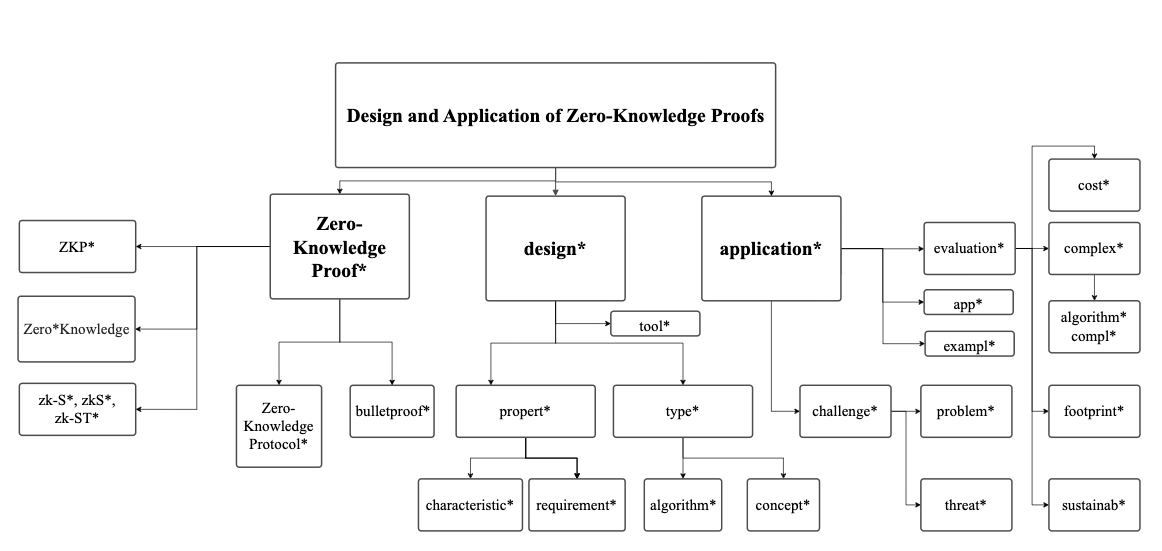
\includegraphics[width=0.99\textwidth]{Pictures/concept map.png}
	\caption{Search compression process}
	\label{fig:concept_map}
\end{figure}

The research question is assigned to topics of Computer Science, Mathematics, and Information Systems. For the search, the databases Web of Science (WoS), Association of Computing Machinery (ACM), zbMATH, arXiV, Association of Information Systems (AIS), and Institute of Electrical and Electronics Engineers (IEEE) were queried. Articles were searched in Title, Keywords, and Abstract, and if possible, with date restrictions back to 2018 (WoS) and 2006 (ACM). The following search string was used: (("ZKP*" OR "Zero-Knowledge*" OR "zero*knowledge*algorithm*" OR "zero*knowledge*protocol*" OR "zero*knowledge*proof*" OR "zkS*" OR "zk*SNA*" OR "zk*STA*" OR "zk*STO" OR "bulletproof*") AND ("application*" OR "example*" OR "app*") AND ("carbon*footprint*" OR "*complexity*" OR "evaluation*" OR "cost*" OR "sustainab*" OR "environment*") AND ("challenge*" OR "threat*" OR "problem*"). After deduplication, the search resulted in 580 hits, which were condensed according to the following approach. First, the result was filtered by English or German resources which have more than or equal to five citations with three times or higher past 180 days usage (560 hits). The next exclusion criteria were applied in Title and Keywords (396 hits), Abstract (319 hits), and Full-text (80 hits), of which backward/forward search added another 20 hits. 

\begin{figure}[hbt]
	\centering
		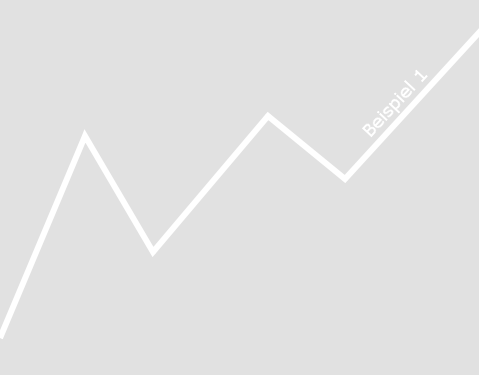
\includegraphics[width=0.99\textwidth]{Pictures/bsp1.png}
	\caption{Concept Matrix}
	\label{fig:concept_matrix}
\end{figure}

Results of the survey can be summarized into the following topics. 
\begin{itemize}
    \item Algorithm design topics: Zero-knowledge proofs are designed by combining proof systems and cryptographic means to achieve specific characteristics. Proof systems are examined and defined, linking and presenting cryptographic tools within the scope of building zero-knowledge argument systems in the area of applicable blockchain-based solutions.
    \item Subsequent to the previous item, most widely used and performative zero-knowledge proofs are described in more detail, i.e., algorithms of specific zk-SNARKs, zk-STARKS, and Bulletproofs.
    \item Selective literature is summarized according to the following problem domains identified: Electronic Voting and Government, Electronic Auctions, Data Queries and Traceability, Electronic Healthcare, Cloud Security, and Scaling.
    \item Opportunities and challenges are summarized and aligned by evaluating and comparing the different algorithms qualitatively through literature review and quantitatively through complexity analysis.
\end{itemize}

\section{Implementation and Evaluation}
Results of this masters' thesis are three artifacts, each satisfying a requirement in project Rapado. The requirements are derived from previous work at the department of Information Systems at Freie Universit{\"a}t Berlin and workshops held within the project consortium. From these broader requirements, specific design requirements are extracted, which can be referred to during implementation. The development of artifacts is conducted in an agile and iterative manner, whereby the demonstration of the technical application of zero-knowledge proofs is at focus. The following table describes the three artifacts and their implementation approach (Table \ref{tab:summary_artifacts}). The project and design requirements are further described in the fourth and sixth chapter. 

The algorithms studied in chapter 5 are evaluated according to their complexity. Artifact 1 represents a reference document to understand zk-SNARKs functionalities. It is shown in the final state after recurring consultation between author and research department. Artifact 2 results from an agile implementation approach and is evaluated through first feedback collection from the project partner. Enhancements are implemented and summarized in chapter 6. Artifact 3 is evaluated by revisiting project and design requirements to assess current and future project needs. 

\setlength{\tabcolsep}{2ex}
\renewcommand{\arraystretch}{1.5}%
\begin{table}[htb]
	\centering
	    \caption{Results and Implementation Description}
		\begin{tabular}{|m{0.001\linewidth} | m{0.12\linewidth} | m{0.35\linewidth} | m{0.4\linewidth} |}
		\hline
		\textbf{}& \textbf{Artifact} & \textbf{Short Description} & \textbf{Implementation} \\ \hline
            1&Groth16 Example \newline Calculation & Step-wise computation of Groth16 protocol by taking a simple polynomial as example. The goal is to create a reference document to underline zk-SNARKs functionality, corresponding to the requirement of accumulating expertise on the topic within the project. & Developed during research phase on zk-SNARKs theory and functionality by taking a simple proof example and following the Groth16 protocol steps \citep{Groth2016OnTS}. \\  \hline
            2&zk-DApp MRO \newline Attestation & Zero-knowledge decentralized application to attest to MRO data of parts and create a trusted verified process. & Agile development with focus of demonstrating the functionality of plonk zk-SNARKs and practical implementation with circom and snarkjs. First feedback is collected and implemented. \\ \hline 
            3&Zero-Knowledge Data \newline Structure & Motivated by recurring comments during workshops and project consortium meetings, this is a first architecture prototype to enable further discussion of effective data formats and digitization of spare parts and corresponding documents. & Analyzing similar efforts in other alternative fields of research \citep{sedlemeirgrenenergy}, key insights are combined with results from the literature survey to implement first ideas and approaches to utilize zero-knowledge proofs to create effective data formats and standards for the future of aviation. \\  \hline 
	\end{tabular}
\label{tab:summary_artifacts}
\end{table}
\begin{comment}
-review of project requirements-->ableiten von design requirements
- with focus at technical functionalities, two use cases were picked out and developed in an agile manner, presenting very first prototypes for open discussion further in the project, main goal of knowledge accumulation is satisfied in chapter 5, designed and implemented artifacts satisfy two other main project requirements
- evaluation according to complexity analysis, fit to the project needs, limitations and future outlook
\end{comment}




\begin{comment}
SLR
Analysis of other resources
--> ends with requirements
(how good/bad the solution is)
-quantitative and qualitative evaluation, e.g. Laufzeit und Interviews 
- say what is not in scope
-DO NOT describe some agile method for the sake of having it! Just say it is a rather agile method etc.

I. Systematic literature review according to vom Brocke, Cooper and Webster: 
    1. Definition of Scope
        - classification, examples, challenges and evaluation methods of zero knowledge proof protocols 
        
    2. Conceptualization
        - work with concept map
        - derive at a search string
        
    3. Literature Search and Selection
        - look for review paper first to get good overview about the topic
        a) exclude paper that are too old and have too few citations and/or low impact factor (e.g. 5.5 is high)
        b) exclusion acc. to title and keywords
        c) exclusion acc. to abstract & structure of paper & RQ
        c) exclusion acc. to full text & availability of resource
        
    4. Synthesizing of Literature
        - cluster definitions, examples, drawbacks and evaluation methods (first suggestion can be found in the preliminary agenda)
        - write overview section about ZKP (Chapter 4)
- - - - - - -
How to know if a paper is useful for me?
1.title 2.keywords 3.abstract 4.structure of the paper 5.examples/use cases 6.research question/formal problem definition
- - - - - - -
% DSR muss nicht sein, kann auch SCRUM oder {"a}hnliches
II. Design Science Research
- DSR method acc. to Peffers and Hevner

\end{comment}
\begin{comment}
2) Ziel der Arbeit, scope of work
- not scope to practically integrate any of the concepts into existing DApp or any other existing system
- welche use cases gibt es f{"u}r ZKPs in RAPADO
- wie k{"o}nnte man diese Umsetzen

4) Ergebnisse skizzieren
- implementation can be a proof of concept, software artifact depends highly on complexity of the use case
\end{comment}
    \clearpage{\pagestyle{empty}\cleardoublepage}
    \chapter{The RAPADO Project}
\section{Project Introduction}
\subsection{Background}
\subsection{Initial Problem Analysis}
\subsection{Project Requirements}
\subsection{Previous Work}
\subsection{Reflection}
\section{Current Project Status}
\subsection{Problem Analysis}
\subsection{Design Requirements}
\subsection{Derived Use Cases}

\begin{comment}

\cite{kliewer2005optimierung}

\begin{table}[bp]
	\centering
		\caption{Beispiel 1 zum Einfügen einer Tabelle}
		\begin{tabular}{| c c c |}
		\hline
			&&\\
			Monat & Linie & Minuten\\
			\hline
			\hline
			&&\\
			Jan & U7 & 10 \\
			Feb & U9 & 12 \\
			Mär & U9 & 20 \\
			\hline
		\end{tabular}

	\label{tab:Beispiel1}
\end{table}


\begin{figure}[tp]
	\centering
		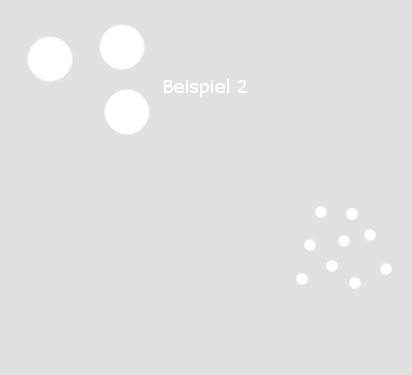
\includegraphics[width=0.50\textwidth]{./Bilder/bsp2.png}
	\caption{Beispiel 2 zum Einfügen einer Grafik}
	\label{fig:bsp2}
\end{figure}
\end{comment}

    \clearpage{\pagestyle{empty}\cleardoublepage}
    \chapter{Zero-Knowledge Proofs}
This chapter surveys selective literature about zero knowledge proofs for practical design application. The goal is to familiarize the reader with the content classification of zero-knowledge proofs in cryptography, and to give an introduction and comparison of main argument systems widely used as of today. Zero-knowledge proof systems belong to the domain of verifiable computation. Verifiable computation (VC) makes use of cryptographic protocols and arguments to verify that a computation was performed correctly. Arguments allow for false proofs only if they require very high computational power. 

The introduction of interactive proof systems by \citet{GoldwasserIPs} and \citet{BabaiIPs} shows that only correct proofs are valid and malicious proving strategies cannot be verified. Traditional proofs are static and are made for easy, step-wise computation verification, whereas IPs require interaction between prover and verifier. In computational complexity theory, interactive proof systems are abstract machines exchanging messages between prover and verifier to convince the verifier that these sets of strings belong to a language \(L\). Here, the formal language \(L\) is defining a decision problem, i.e., a computational problem that has only two outputs, yes and no. Examples of sets of strings in \(L\) can be, that a certain Bitcoin transaction is valid, \(x = 7\) for a given \(f(x)\), or a certain object belongs to a specific merkle tree. The untrusted prover has unlimited computational power and the verifier is honest and computationally restricted. Advances in computational complexity theory during that time showed that IPs are more efficient and belong to a wider class than the traditional \textbf{NP}, i.e., problems solvable in deterministic polynomial time by reading proof strings of polynomial length \citep{SassonIOPsinproceedings}. In 1987, it was shown that every language belonging to NP has zero-knowledge proof systems \citep{anymental10.1145/28395.28420}. Later, it was shown that the class of \textbf{IP}, i.e., problems solvable by interactive proof systems, lies in \textbf{PSPACE}, i.e., problems solvable in polynomial space \citep{Shamir10.1145/146585.146609}, and that every language \(L\) in polynomial time has an interactive proof system \citep{Lund10.1145/146585.146605}. The complexity class of IP describes prover and verifier interaction in a polynomial number of rounds. Other important advances in computational complexity theory are \textbf{MIP=NEXP} \citep{Laszlo} and the \textbf{PCP theorem} \citep{PCPTheorem10.1145/278298.278306}. These works resulted in a set of proof and argument systems, that will be introduced in this chapter. \citet{Thaler} gives a further, exhaustive overview of all systems and in-depth protocol descriptions. 

The examined proof systems are secure against computationally unrestricted provers: \textit{Interactive Proof (IP), Multi-prover Interactive Proof (MIP), linear Probabilistically Checkable Proof (PCP), and Interactive Oracle Proof (IOP)}. 

Combining the systems above with cryptographic tools to force certain behavior in the proof generation will create an argument system. Argument systems are considered to be zero-knowledge, if and only if the proof does not reveal anything but its own validity \citep{GMR89}. Adding certain properties, e.g. non-interactivity, succinctness, and knowledge, will design a certain argument of knowledge, e.g. zk-SNARK (zero-knowledge succinct non-interactive argument of knowledge). Different zk-SNARKS and notions will be examined in more detail.

The next sub chapters are structured according to the design approach described above. First, IPs, MIPs, PCPs, and IOPs will be defined. Through the combination with polynomial commitment schemes argument systems can be designed. Non-interactivity is achieved through Fiat-Shamir transformation. Second, properties and mathematical tools will be introduced to describe different arguments of knowledge: zk-SNARK, FRI-STARK and bulletproofs. Third, real-world applications of zero-knowledge proof systems will be summarized. Lastly, the different proof systems will be evaluated in different application scenarios.

\begin{comment}
- what is zero knowledge definition
- what means indistinguishable
- different types of zero-knowledge (perfect, statistical, computational)
- ZKPs are part of verifiable computations
- what is verifiable computation
\end{comment}

\section{From Proof Systems towards Argument Systems}

A mathematical proof in the context of computer science and cryptography is any object that convinces a verifier that a statement is correct. Mathematical proofs embody what is defined in the complexity class NP. A proof system is a structured scheme that outputs a decision of whether a statement is correct or incorrect. In general, there are three properties that are desirable for proof systems \citep{GoldwasserIPs}, which will be introduced shortly. Throughout this sub chapter, these properties will be revisited more exhaustively.

\begin{align*}
    \text{\parbox{370}{
    1. The procedure to create and verify proofs should be efficient and fast. \\
    2. \textit{Soundness}: If a statement is incorrect, there is no possibility of it having a convincing proof. \\
    3. \textit{Completeness}: True statements should have a convincing proof of their validity. \\}}
\end{align*}

Unlike argument systems, proof systems do not limit the malicious prover in its computational power (\textit{statistical soundness}). Using cryptographic primitives and restricting the prover, e.g., probabilistic polynomial time proof, so that it cannot break the primitives, describes the design towards argument systems, which are computationally sound \citep{ArgSystems, MicaliArgSys}. Each proof system presented makes assumptions on the prover. However, only with the use of cryptographic tools and zero-knowledge, these proof systems can be extended with additional properties to yield zero-knowledge argument systems of various kinds.

\begin{comment}
IPs are the basis to understand cryptographic protocols and argument systems
argument systems are IP with a specific assumption
polynomial IOPs together with polynomial commitment scheme always yields a specific argument of knowledge, can be made non interactive with fiat-shamir, can be succinct too, different abwandlungen
but before we need basic understanding on different proof systems that lie behind the construction of argument systems
then we need understanding of commitment scheme and fiat shamir transform
how zero knowledge is applied in the design will be shown later when going through the different systems

information secure = only theoretically
what are those, little history
1:polynomial IOPs 
- interactive proofs intro
- MIPs
- constant round IOPs
2:linear PCPs
-intro from the book Thaler-->combined with cryptographic primitives we get SNARKs, everything is a SNARK and SNARK variation
-Luong and Park: properties intro
- Yang Yang et al properties
-Soonhyeong 2021: better verification with EVM to verify non-maliciousness of blocks (zKSNARKS used)
\end{comment}

\subsection{Interactive Proofs}

In interactive proof systems, the prover with unlimited computational resources interacts with a computationally bound verifier in order to convince the verifier of the correctness of a statement. The verifier randomly challenges the prover, which is referred to as coin tosses \citep{GoldwasserCoinTosses}. These challenges happen in rounds, until there are sufficient tests run and the verifier is convinced. \citet{GoldwasserIPs} defined an interactive proof system that is private, i.e., that the verifiers challenges are not publicly accessible, whereas the interactive proof system of \citet{BabaiIPs} allows the coin tosses to be publicly accessible by the prover.
\begin{align*}
    \text{\parbox{450pt}{\textbf{Interactive Proof System.} \textit{\(L\) is a language over \(\{0,1\}^n\), with n representing the input size domain of n-bit strings. An interactive protocol is a interactive proof system if after \(k\) rounds, the probabilistic verifier in polynomial time exchanged \(k\) messages with the computationally unrestricted prover, and has to either accept or decline the correctness of the prover's proposition. IP is the complexity class of problems solvable by a k-round interactive proof system.}}}
\end{align*}
  
The transcript is the order in which messages are exchanged. The prover and verifier are functions \(P(x), V(x)\) with common input \(x\). The overall distribution of all transcriptions between prover and verifier is called \(View_V(P(x), V(x))\), which is bound by the number of rounds between \(P\)and \(V\). \(P\) provides a result that satisfies the proposition, e.g., \(y\) to a function \(f(x) = y\). \(P\) and \(V\) exchange a transcript of messages \((m_1, m_2, m_3, ..., m_k)\), whereby both parties take turns and the last message is sent by the prover. Note, that \(V\) is probabilistic with internal randomness \(r\). Hence, the output depends on \((V, x, r, P)\) and is \(\{0,1\}\), i.e., \(1\) if the statement is correct, and \(0\) if it is incorrect \citep{GoldwasserIPs, BabaiIPs}. Interactive proof systems have completeness error \(\delta_c\) and soundness error \(\delta_s\) . For any input \(x\), there must be a convincing proof that \(f(x)\) is correct. Incorrect statements for \(y \neq f(x)\) cannot result in a convincing proof, i.e., a malicious prover does not exist \citep{Thaler}. IP systems are valid if \(\delta_c, \delta_s \leq 1/3\).

\subsubsection{Non-interactive, publicly verifiable arguments}
The Fiat-Shamir Transformation takes any interactive proof system based on public coin tosses and transforms it into a non-interactive, publicly verifiable system. This transformation can be described effectively with the use of an ideal cryptographic assumption called \textit{Random Oracle Model (ROM)}. 
\subsubsection{Random Oracle Model}
\subsubsection{Fiat-Shamir Transformation}
\begin{comment}
introduced by  GOLDWASSER, Shafi; MICALI, Silvio; RACKOFF, Charles. The
knowledge complexity of interactive proof systems. SIAM Journal
on computing. 1989, vol. 18, no. 1, pp. 186–208.
GKR protocol-->why? GKR protocol is general-purpose in the sense that it solves the problem of arithmetic circuit evaluation, and any problem in P can
be “efficiently” reduced to circuit evaluation
randomness
completeness
soundness
statistical soundness
computational soundness
fiat shamir transformation for non interactive
knowledge soundness
proof of knowledge
obtaining zero knowledge from it: verifier learns nothing about the witness
\end{comment}



\subsection{MIPs}
\subsection{Linear PCPs}
\subsection{constant round IOPs}
\subsection{Polynomial IOPs}
(focus on chapter 10.6, combine with preliminaries from previous chapters in Thaler)

\section{Towards zero-knowledge non-interactive arguments of knowledge}
-first succinct argument of knowledge by goldwasser etc. 
-what is succinct
- repeat that Fiat Shamir Transformation can make them all non-interactive
-every proof from above combined with polynomial commitment schemes yields a SNARK
-short explanation what are polynomial commitment schemes: %https://coingeek.com/how-plonk-works-part-1/#:~:text=PLONK%20is%20a%20state%2Dof,by%20all%20circuits%5B1%5D.
- how: 1 design a public-coin polynomial IOP for circuit- or R1CS-satisfiability, 2 use polynomial commitment scheme 3 remove interaction via fiat shamir
- linear PCPs are exception: they need to be combined with pairing based cryptography
- everything is a sub of SNARKs
- I only want to cover three most practical zero knowledge SNARKs
- Constant-round IOPs vs. MIPs and IPs-->p.301 Thaler
- every combo with polynomial commitment scheme is a SNARK
- we focus on Groth16, PLONK, FRI-STARK, bulletproof

NITULESCU, Anca. zk-SNARKs: A Gentle Introduction [https:
/ / www . di . ens . fr / ~nitulesc / files / Survey - SNARKs . pdf].
2020. Tech. rep. ENS Paris. Accessed: 2022-05-15.

\subsection{Circuit-specific zk-SNARK}
- implementation of zero-knowledge argument systems was not possible until very recently, with advances in blockchain technology
- Linear PCP and pairing based cryptography
- definitions
- R1CS, QAP and Elliptic Curve Pairing
- main functionalities: trusted setup, proof and verify
- history
- Groth16
- performance enhancements by Groth\& Maller 2017, Lipmaa 2019 and Kim Lee Oh 2020 as the newest contribution with only one single verification
- Luong and Park easy Intro
- Yang Yang et al: Intro Groth16, R1C1, QAP easy examples
- Baghery et al. mathematical backings if needed
- Benamara: ECs and pairings, good math paper 
- Guo et al: QAP, Bilinear Maps, R1CS theory



\subsection{Towards Universal Setup zk-SNARK}
PLONK
Constant round polynomial IOP plus Kate commitment
-definitions
-history
-plonk, it is a SNARK
-main functionality

\subsection{FRI-STARK}
with FRI-based polynomial commitment
-does not use R1CS
-fri starks
-Salleras et al 2021

\subsection{Bulletproofs}
with discrete-log based polynomial commitment
- uses R1CS too
- they are non-interactive,
- they are zk arguments of knowledge
- Godden et al bulletproofs
- Chung et. al bulletproof+
- Deng at al history of bulletproofs
-Salleras et al 2021
main protocols: Lipmaa, Boudot, then Groth and Coutueau, then Hybrid from Kim Lee 2019
Deng et al 2022: history of range proofs, cuproof as example
-Kim Lee 2019: overview on range proof protocols


\section{Opportunities and Use Cases}

-e-government:e-voting/digital election

-healthcare: purchasing medical insurance contracts, patient data exchange/access
-e-auction/bidding systems
-cloud computing: zk port knocking, data deduplication, authentication schemes for cloud servers
-blockchain scaling: decrease comp cost for tx verification, zkRollups, zkSync
-querying: link traversal, zk-SQL SPARQL queries, zk based traceability systems

- Sedlmeier et al: overcoming transparency vs. privacy
- Godden et al overview of ZKP use cases: verifiable comp., linked data, identity management, access control
- ZKPs belong to verifiable computation, succinct blockchain Simunic et al 2022
- sources from Zhang et al 2021 PipeZK overview of the different Anwendungsbereiche of ZKPs-->what is verifiable outsourcing as application example?
- Maller et al 2019 Sonic: verifiable outsourcing computation example paper

\subsection{Identity Protection and Authentication}
- Bonsad et al use case
- Guo et al: e-government example
- Wang et al: hospital as trusted party, insurance receives proofs and cashes out, patient's medical data protected at all times
- Shi et al (2022): Schnorr ZKP used to proof user identity-->a bit old fashioned ZKP used maybe??
- Hunag et al 2020: good use case for MRO data sharing? zk SNARKS
- Major,Buchanan(2020): port knocking authentication scheme
- Kanagamani, Karuppiah(2021): data deduplication cloud computing with in-line block matching and ZKP properties
-Soonhyeong 2021: better verification with EVM to verify non-maliciousness of blocks (zKSNARKS used)
- Munivel Kannammal (2019): authentication scheme as additional security to prevent mobile phone password attacks on cloud storage server
- Liu Wang Peng Xing 2019: remote authentication for mobile cloud computing
-cloud computing
-egovernment, eauctions


\subsection{Data Sharing and Traceability}
- Xue and Wang: traceability use case applicable to pred. maintenance problem
-link traversal, SQL
-healthcare
-zero knowledge static program analysis: proof that a secret code is correct (Fang, Near, Darias, Zhang 2021)

\subsection{Blockchain Scaling}
- zk Roll ups, more sources needed
- Xu Chen(2021): new algorithms for zero knowledge set membership for ZK-scaling, based and compared to zkSync
- 
\section{Challenges}
- challenges can go into evaluation/comparisons of the 4 zkps
\subsection{Cost}
-Zhang et al 2021 PipeZK time and cost challenges of zKSNARK
-effieciency of ZKP: computation depends on field size-->there is a need for memory efficient ZKPs: wolverine and mac'n'cheese can do it better, but QuickSilver better protocol for large circuits (Yang, Weng, Sarkar, Wang 2021), Dittmer et al (2022) outperform Quicksilver then (most current best performing memory based protocol)
-elements from Sedlmeier Völter Strüker (2021): take the cost of Groth16

\subsection{Trust Assumption}
-Huang et al 2020 semi trusted proxy server, their assumptions
-trusted set up for zk Snarks

\subsection{Quantum Computing Threats}
1. Why are quantum verifiers a threat? (maybe Katz et al 2018)
2. different aspects of solution examples
-Deng et al 
- Xie Yang 2019: quantum secure CRS, good arguments of other shortcomings of ZKP systems, interactive and non interactive quantum zero knowledge proof systems
- Vidick Zhang 2020: describe the three problems that there are protocols developed for (big umbrella problem: quantum verification problem), good definitions from the quantum world
- also include Watrous(2009)-->coming from Vidick Zhang 2020
-Lyubashevsky et al (2020): new lattice based ZKP algorithm which is the fastest and smallest proof size for small int addition and multiplication 

\section{Evaluation Methods}
-Huang et al 2020: 1)privacy preserving and security: confidentiality, availability, integrity, privacy-preserving, traceability, single point of failure 2) performance evaluation: computing cost, number of startup nodes, privacy protection, time to generate NIZK keypair, NIZK proof, verify NIZK proof
-Zhang et al 2021 PipeZK proof generation enhancement
- Maller et al 2019 Sonic: better structured SRS in linear size to speed up proof verification

\subsection{Performance Analysis}
-Liu et al, Zheng at al: semihonest model evaluation topics-> computational complexity, communication complexity, experimental evaluation
- Liu Wang Peng Xing 2019: remote authentication for mobile cloud computing, Real-Or-Random model and BAN logic for security evaluation REGARDING different attacks
- Zhang et al 2021 PikeZK: new hardware accelerator to boost comp time for proof generation

\subsection{Sustainability}
-maybe too little literature for an own sub chapter
-Simunic et al mention need for more sustainable solutions in blockchain privacy preserving through ZKPs
-elements from Sedlmeier Völter Strüker (2021): ZKPs are more sustainable 
    \clearpage{\pagestyle{empty}\cleardoublepage}
    \chapter{Implementation and Results}
\section{Groth16 proof and verification}
Let us use an example to illustrate the underlying mathematical methods that are applied in zk-SNARK. The example calculation will use the KoE assumption for simplification. In practice, the FFT is applied. First, the arithmetic circuit is transformed into a R1CS. The R1CS is used to obtain the QAP. Homomorphic hiding, elliptic curves and pairing-based cryptography are introduced in more detail and put in context for the next steps of the calculation. Finally, the Groth16 protocol is introduced: First, the key generation steps are explained. Second, the proof is generated. Lastly, the verification steps are illustrated. Formal definitions are found in 5.2.

Say we want to prove we know a secret x so that

\[x^3 + x + 5 = 35\]

In this case, our secret is x = 3.
In practice, we would use hiding and modular arithmetic instead of real numbers and calculations since these are easy to forge and find solutions to, which will make the proof useless. For R1CS and QAP we will proceed with real numbers examples to show the underlying mechanisms. The following will demonstrate how any computation that needs to be proven can be converted into polynomial format.

\subsubsection{Arriving at a R1CS}

A rank-1 constraint system is a mathematical format to help us reduce our problem into a less complex computational problem. First, we flatten the equation by writing a short program that would break down the different steps to solve the equation.

\begin{enumerate}
    \item \(sum1 = x * x\)
    \item \(y = sum1 * x\)
    \item \(sum2 = y + x\)
    \item \(out = sum2 + 5\)
\end{enumerate}

As shown above, we arrive at an arithmetic circuit with 4 gates and the solution variables
\[x = 3, y = 27, sum1 = 9, sum2 = 30, out = 35.\]

From this, we can construct the solution vector \(s\) , which has to start with a dummy variable of value 1, which we call \textit{one}.
Now, the solution vector \(s\) is
\begin{align}
    \Vec{s} &= \begin{pmatrix}
     one \\ x \\ out \\ sum1 \\ y \\ sum2
\end{pmatrix}
\end{align}
Each gate will be represented so that
\begin{align}
     \Vec{s}\cdot\Vec{a_i} * \Vec{s}\cdot\Vec{b_i} - \Vec{s}\cdot\Vec{c_i} = 0
\end{align}

Let us go through every gate and assign the values for a, b and c.
For the first gate \(sum1 = x*x\), the values of a, b and c are assigned as follows:
\begin{align*}
    a_1 &=\begin{bmatrix}
        0 & 1 & 0 & 0 & 0 & 0
    \end{bmatrix}
\end{align*}
\begin{align*}
    b_1&=\begin{bmatrix}
        0 & 1 & 0 & 0 & 0 & 0 
    \end{bmatrix}
\end{align*}
\begin{align*}
    c_1&=\begin{bmatrix}
        0 & 0 & 0 & 1 & 0 & 0
    \end{bmatrix}
\end{align*}

This is correct, because the dot product of s and a, multiplied by the dot product of a and b, subtracted by the dot product of s and c is 0 (6.2).

This procedure is applied to every gate. Let us show more complex gates to underline the calculation. For example, the third gate and the fourth gate. The third gate \(sum2=y+x\) could be approached as the first gate, by setting the variables in the equation to 1. However, this would not fulfill the equation shown in (6.2). Therefore, the correct values for \(a_3, b_3 \text{ and }c_3\) are
\begin{align*}
    a_3 &=\begin{bmatrix}
        0 & 1 & 0 & 0 & 0 & 0
    \end{bmatrix}
\end{align*}
\begin{align*}
    b_3&=\begin{bmatrix}
        1 & 0 & 0 & 0 & 0 & 0 
    \end{bmatrix}
\end{align*}
\begin{align*}
    c_3&=\begin{bmatrix}
        0 & 0 & 0 & 0 & 0 & 1
    \end{bmatrix}
\end{align*}

Here, we make use of the dummy vector \textit{one}, so that we can arrive at 
\[30 * 1 - 30 = 0.\]

The fourth gate \(out=sum2+5\) also has to be approached by holding true to the dot product equation in (6.2) as well. We have to make use of the dummy vector once again. Setting the values of \(one, sum2 \text{ and } out\)  to 1 will give us the following incorrect solution:
\begin{align*}
     \Vec{s}\cdot\Vec{a_4} * \Vec{s}\cdot\Vec{b_4} - \Vec{s}\cdot\Vec{c_4} \neq 0.
\end{align*}
The calculation shows \(30 * 1 - 35 \neq 0\), which means we need to add 5, so that the dot product of vector \(s \text{ and } a\) adds up to 35. Therefore, the values of \(a_4, b_4 \text{ and }c_4\) are as follows:
\begin{align*}
    a &=\begin{bmatrix}
        5 & 0 & 0 & 0 & 0 & 1
    \end{bmatrix}
\end{align*}
\begin{align*}
    b&=\begin{bmatrix}
        1 & 0 & 0 & 0 & 0 & 0 
    \end{bmatrix}
\end{align*}
\begin{align*}
    c&=\begin{bmatrix}
        0 & 0 & 1 & 0 & 0 & 0
    \end{bmatrix}
\end{align*}

By combining our results into matrices, we can set up the corresponding R1CS:

\begin{align}
A&=\begin{pmatrix}
    0 & 1 & 0 & 0 & 0 & 0 \\
    0 & 0 & 0 & 1 & 0 & 0 \\
    0 & 1 & 0 & 0 & 1 & 0 \\
    5 & 0 & 0 & 0 & 0 & 1
\end{pmatrix}
\end{align}
\begin{align*}
B&=\begin{pmatrix}
    0 & 1 & 0 & 0 & 0 & 0 \\
    0 & 1 & 0 & 0 & 0 & 0 \\
    1 & 1 & 0 & 0 & 0 & 0 \\
    1 & 0 & 0 & 0 & 0 & 0
\end{pmatrix}
\end{align*}
\begin{align*}
C&=\begin{pmatrix}
    0 & 0 & 0 & 1 & 0 & 0 \\
    0 & 0 & 0 & 0 & 1 & 0 \\
    0 & 0 & 0 & 0 & 0 & 0 \\
    0 & 0 & 1 & 0 & 0 & 0
\end{pmatrix}
\end{align*}

\subsubsection{From R1CS to QAP}

The R1CS shows three matrices \(A, B \text{ and }C\) representing the four gates each of length six. It is transformed into a QAP by expressing polynomials as sums of Lagrange Interpolation (chapter 5.2.2). This results in three sets of polynomials \(A_i(X), B_i(X) \text{ and }C_i(X)\) each consisting of six polynomials of degree three. In the following, we will summarize the reason of setting up a QAP instead of continuing with the R1CS. Lagrange Interpolation allows us to come up with polynomial coefficients, which represent each gate, when evaluated at an X in the range of number of constraints (gates). With X = 1, the Lagrange Interpolation can be explained quite well, because it means that we can just add up the coefficients of the polynomials in \(A_i(X), B_i(X) \text{ and }C_i(X)\). Each set of polynomial is built so that evaluated at a gate X, whereby X has to be in the range of the number of gates (constraints), will deliver the specific value of X and 0 for the other values in that specific range.\newline
The QAP for our example:
\begin{align*}
    A_i(X) \\
    \begin{bmatrix}
        -5.0 & 9.166 & -5.0 & 0.833 \\
        8.0 & -11.33 & 5.0 & -0.666 \\
        0.0 & 0.0 & 0.0 & 0.0 \\
        -6.0 & 0.5 & -4.0 & 0.5 \\
        4.0 & -7.0 & 3.5 & -0.5 \\
        -1.0 & 1.833 & -1.0 & 0.166
    \end{bmatrix} \\
\end{align*}
\begin{align*}
        B_i(X) \\
    \begin{bmatrix}
        3.0 & -5.166 & 2.5 & -0.333 \\
        -2.0 & 5.166 & -2.5 & 0.333 \\
        0.0 & 0.0 & 0.0 & 0.0 \\
        0.0 & 0.0 & 0.0 & 0.0 \\
        0.0 & 0.0 & 0.0 & 0.0 \\
        0.0 & 0.0 & 0.0 & 0.0
    \end{bmatrix}
\end{align*}
\begin{align*}
        C_i(X) \\
    \begin{bmatrix}
        0.0 & 0.0 & 0.0 & 0.0 \\
        0.0 & 0.0 & 0.0 & 0.0 \\
        -1.0 & 1.833 & -1.0 & 0.166 \\
        4.0 & -4.833 & 1.5 & -0.166 \\
        -6.0 & 9.5 & -4.0 & 0.5 \\
        4.0 & -7.0 & 3.5 & -0.5
    \end{bmatrix}
\end{align*}
The corresponding values in the matrices represent polynomial coefficients and shall be read from right to left, e.g. \(A1(X) = 0.833x^3 - 5x^2 + 9.166x -5\). For example:
\begin{align}
     X = 1 \\
    A1(1) = 0, A2(1) = 1, A3(1) = 0, A4(1) = 0, A5(1) = 0, A6(1) = 0
\end{align}
Comparing the results with the first vector a of the first gate, we see that the results represent the first gate.
For example, evaluating \(A, B \text{ and }C\) at X = 1 means to adding up the coefficients of the first polynomial of \(A\) , which will result in a value matching to the vector value in the first gate. Then, the next polynomial in A etc. It will result in a vector of length six and will be correct if the values match vector a from the first gate in our R1CS. The same is done by evaluating the polynomials with X, whereby X starts at 1 and ends at the number of gates, in our case \(X=\{1,2,3,4\}\).
However, it would be cumbersome to evaluate each constraint individually. This is why we can make use of the QAP to check whether the dot product equation of the polynomials will hold:
\begin{align}
    A_i(X)\cdot \Vec{s} * B_i(X)\cdot \Vec{s} - C_i(X)\cdot \Vec{s} = H(X) * Z(X)
\end{align}
Interestingly, the left side of the equation is our target polynomial \(T(X)\), which we want to proof.
Now, let's have a look at the right side of the equation in (6.6). \(Z(X)\) is known if we know the number of constraints. In Groth16, it is made available in the trusted setup. In this case, we have four gates, so we arrive at
\begin{align}
    Z(X) = (x-1)(x-2)(x-3)(x-4)
\end{align}
\(H(X)\) is the hiding of our initial minimal example, those input we don't want to share, but prove we know the solution to. What role hiding plays will be explained shortly. Now, we want to still finish looking at the equation in (6.6). In essence, we want to proof we know a polynomial and its solution, so that
\begin{align}
    T(X) / Z(X) = H(X)
\end{align}
Ultimately, in our example, \(H(X)\) is also a polynomial. We know the QAP is correct, if \(H(X)\) is a polynomial without remainder. In this example, the resulting
\[H(X) = -0.44x^3 + 17.055x^2 - 3.666x.\]

Practically, the coefficients of each polynomial in \(A_i(X), B_i(X) \text{ and }C_i(X)\) are publicly known. The same can be said for \(Z(X)\) through knowing the number of constraints (in this example we have four constraints). The prover can calculate the coefficients of \(H(X)\) by dividing T(X) / \(Z(X)\). However, there is no zero-knowledge yet, since the prover has to prove knowledge of vector \(s\) and \(H(X)\) without revealing it.
\newpage

\subsubsection{Hiding}
Zk-SNARKs are dependent on a trusted setup releasing these parameters. The goal is to prove knowledge of the polynomial \(H(X)\) with all its coefficients without disclosing any of this information. Therefore, the trusted setup also provides a random secret point \(P\). Note, that \(P\) is hashed, calculated once and deleted from memory. Depending on the number of constraints, a certain amount of \(P\) values are needed. In our example, we have four constraints, which need \(P = {1, P, P^2, P^3}\), whereby the value of \(P^3\) corresponds to the value of \(x^3\) when the polynomials are evaluated. The following values of \(P\) are provided

\begin{align}
    hh(1), hh(P), hh(P^2), ..., hh(P^\textsuperscript{(no. of constraints - 1)})
\end{align}

The trusted setup makes these values publicly available in the CRS.

With our previous knowledge, we know that the prove will consist of
\begin{align}
    \frac{hh[A(P)] * hh[B(P)] - hh[C(P)])}{hh[Z(P)]} = hh[H(P)]
\end{align}

The hidings of our polynomials are numbers, that currently can just be forged. The following will show how it can be proven that these numbers are hidings of the polynomials \(A(X)\), \(B(X)\) and \(C(X)\) in \(P\) which is not known to anybody. Furthermore, we need to prove that in order to arrive at \(A(X)\), \(B(X)\) and \(C(X)\), the same solution vector \(s\) was used (6.6). 

In order to approach the first problem, proving that the hidings of \(A(X)\),  \(B(X)\) and \(C(X)\) were actually calculated in \(P\), we need to "extend" \(P\) by the same number, namely \(u\). The CRS consists also of \(hh(u*P), hh(u*P^2), hh(u*P^3)\), etc., i.e., it consists of two sets of hidings. We know that \(A(X)\) is a linear combination of the values of vector s inserted into the polynomials A1, A2, A3, etc. of A. B calculating \(hh[A(P)]\) and \(hh[A(u*P)]\) and looking if \(hh[A(P)] = u * hh[A(u*P]\) holds true, shows that the hiding of \(A(X)\) calculated in \(P\)is indeed a result of linear combination of A1, A2, A3, etc. and the values of the vector s (6.6). All we did is to prove that the same sets of hidings of \(P\)were use to arrive at these numbers. The same is applied to the hidings of \(B(X)\), \(C(X)\) in P.

For the second problem, to prove the same values of vector s were used to arrive at the hidings of \(A(X)\), \(B(X)\) and C(X) in \(P\) a similar approach can be used. In our example, vector s has six solution variables. We use a new variable K as
\begin{align}
    K = K1 + K2 + K3 + K4 + K5 + K6
\end{align}
\begin{align*}
    K1 = A1(P) + B1(P) + C1(P)\\K2 = A2(P) + B2(P) + C2(P)
\end{align*}
\begin{center}
    ... \\
\end{center}
\begin{align*}
    K6 = A6(P) + B6(P) + C6(P)
\end{align*}
By checking that 
\begin{align}
    hh[K(P)] = one*hh[K1] + x * hh[K2] + out * hh[K3] + ... + sum2 * hh[K6],
\end{align}
we can prove that indeed the same coefficients of vector s were used. This way it is nearly impossible to come up with numbers that hold true for another \(P\)and to create proofs without the knowledge of the coefficients.

\subsubsection{Homomorphic Hiding}

\(y = hh(x)\) is a hashing function. It is collision resistant, i.e., one cannot guess anything of x from y. For zero-knowledge proofs, this property alone is not sufficient. The hashing function should also preserve algebraic structures, so the checks in , e.g., (6.10) can be performed. Let us divide the term \textit{Homomorphic Hiding} into two sections to explain in more detail.

A function \(y = hh(x) = e^x\) is homomorphic if
\begin{align}
    hh(a*x1 + b*x2) = e^\textsuperscript{a*x1+b*x2} = e^\textsuperscript{a*x1} * e^\textsuperscript{b*x2} = hh(x1)^a * hh(x2)^b
\end{align}
As seen in (6.13), the basic exponential laws hold. However, this function is not hiding, because one could calculate the logarithmic base e of x, because of working with only real numbers \begin{math}\mathbb{R}  
\end{math} so far.

We need to express variables in a finite field as of modulo p with p being a large prime. The finite field consists only of integer inputs in the range of 1 and some value p-2. This way, expressing values in modular arithmetic, nobody can guess or calculate our base e anymore. Now,
\begin{align}
    y = hh(x) = G^x,
\end{align}
where G is a value in the finite field \begin{math}\mathbb{F}_p\end{math} and y will always be expressed as modulo p.

With homomorphic hiding being introduced, we know all the tools being used to prove that we can calculate the equation in (6.8) with the polynomials from the QAP and the same values of vector s, without knowing any \(P\)and u * P. We know how the proof is calculated without revealing our solution vector s. The following deals with the verification if the above equations hold true, without revealing the solution vector s.

\subsubsection{Elliptic Curve Pairing}

The goal of PCP and pairing-based zero-knowledge algorithms is to create a succinct proof, that a defined computation with given inputs produces certain known outputs, without revealing any information about them and to show that the constraints of that computation hold. Eventually, we want to check if the following equality holds true, i.e., that after transforming our problem into polynomial structure, we know some polynomials so that

\begin{align}
    \frac{A(x) * B(x)}{Z(x)} = H(x) + C(x)
\end{align}

We have the polynomials \(A, B \text{ and }C\), not expressed in real numbers, but mapped to a finite field with a large prime number. We can calculate \(H(X)\) as in (6.8). Now, we are going to use generators for each of our polynomial to produce points on an elliptic curve. This is necessary to make use of pairing, which allows us to check if equations, e.g., (6.13), hold true without knowing the actual variable values in these equations. In the following, some preliminaries will be introduced to create a basis for the Groth16 CRS generation, and proofing and verification mechanism.

Elliptic curves are used to define collision resistant one-way functions, i.e., homomorphic hiding functions. An elliptic curve is a polynomial, e.g., the elliptic curve used in Bitcoin (Figure 1). 

\begin{figure}
\centering
\begin{minipage}{.5\textwidth}
  \centering
  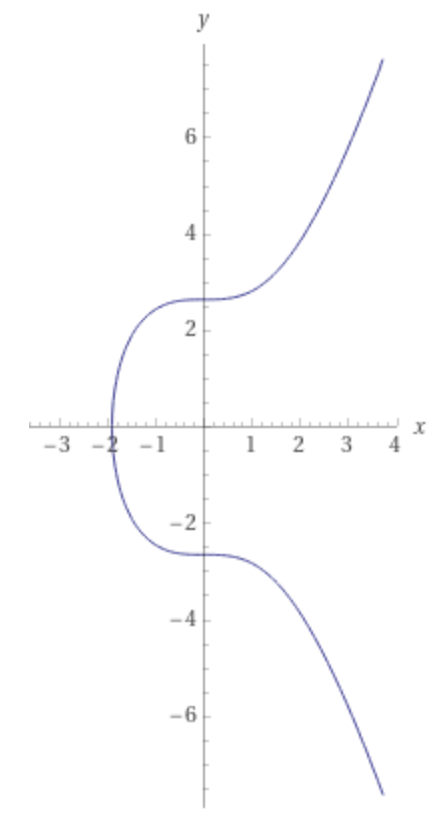
\includegraphics[width=.4\linewidth]{Pictures/bitcoinec.png}
  \caption{Figure 1:\ \(y^2 = x^3 +7\)}
  \label{fig:test1}
\end{minipage}%
\begin{minipage}{.5\textwidth}
  \centering
  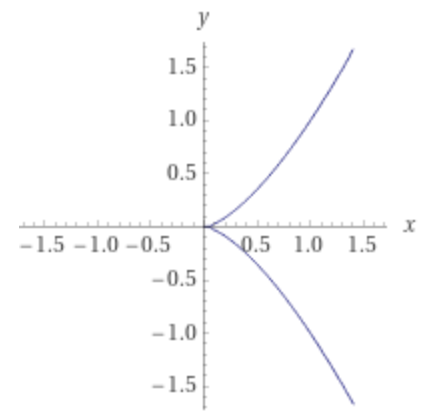
\includegraphics[width=.4\linewidth]{Pictures/y2x3.png}
  \caption{Figure 2:\ \(y^2 = x^3\)}
  \label{fig:test2}
\end{minipage}
\end{figure}

Elliptic curves are useful for zk-SNARKs because of the discrete logarithm problem, which is believed to be very hard to solve. Given a point \(g\) on the elliptic curve, and a multiple of that point, \(n*g\), it is impossible to solve n, even if \(g\) and \(n*g\) are given. In order to choose an elliptic curve that offers homomorphic hiding, we need to implement a mapping between our known numbers of the finite field \begin{math}\mathbb{F}_p\end{math} and a set of points on the elliptic curve (hidden space). Let \begin{math}\mathbb{F}_p\end{math} be a finite field of order p, whereby p is a large prime, e.g., if \(p=97\), then \begin{math}\mathbb{F}_p\end{math} \(=\{0, 1, 2, 3, ..., 96\}\) For this, we are going to take a generator point \(g = (x1,y1)\) that lies on the elliptic curve and multiply it with every element \({element}_i\) in \begin{math}\mathbb{F}_p\end{math}. For example, \(g + g = 2*g\) is calculated by putting a tangent line on \(g\), and wherever the line crosses the elliptic curve, we receive the result by using the opposite signs of that point. To arrive at \(2*g + g = 3*g\), the point \(2*g\) is used to draw a line to \(g\), see where the line further intersects with the elliptic curve, and use the opposite signs of that point to arrive at \(3*g\). This is repeated for every \(element\) in \begin{math}\mathbb{F}_p\end{math}. As a result, we have our finite field mapped to a hidden space on the elliptic curve. In summary, every \(element\) is hidden by
\begin{align}
    hh(element) = element * g
\end{align}
Additionally, we have to define what 0 and 1 are. The element 0 is the subtraction of a point on the elliptic curve, i.e., when point g goes to infinite. 1 is the point g itself.
Now, we have achieved homomorphic addition:
\begin{align}
    (A + B) \longrightarrow (A + B) * g = A*g + B*g
\end{align}

In order to use elliptic curve pairing to verify zk-SNARKs proofs, e.g., Groth16, we need to achieve a limited homomorphic multiplication operator. The hidden space is a group of points generated by the finite field elements and the generation point, \(g1\) on the elliptic curve. Now, we want to choose a subgroup \begin{math} \mathbb{G}_1\end{math} from that group. We choose that subgroup in a away that the number of elements we chose, \(r\), is a prime number too. Having found r, we can continue to choose the embedding degree of the elliptic curve. In Groth16, the proving key and verification key consist of \begin{math} \mathbb{G}_1\end{math} and \begin{math} \mathbb{G}_2\end{math} element. The embedding degree \(k\) has to be found in a way that \(p^k-1\ |\ r\), i.e., is a multiple of. Let us use a minimal example to show how to arrive at \begin{math} \mathbb{G}_1\end{math} and \begin{math} \mathbb{G}_2\end{math}.
Let us define an example base field \begin{math}\mathbb{F}_p\end{math} \(= \{0,1,2\}\) with \(p = 3\). We have found an embedding degree \(k=2\). In order to achieve our goal of creating a subgroup \begin{math} \mathbb{G}_2\end{math}, we need to extend our base field by a defining polynomial. This polynomial is of degree \(k\), and no element of our base field evaluates it to 0. In summary, we have:

\begin{align}
    \mathbb{F}_p = \{0,1,2\}, p = 3, k = 2
\end{align}

Defining polynomial for field extension \begin{math}\mathbb{F}_p^k\end{math}: 
\begin{align*}
    f(x) = z^2 +1 \\
    f(0) = 1\\
    f(1) = 2\\
    f(2) = 5 mod 3 = 2
\end{align*}

As shown in (6.18), none of the base field elements make f(x) evaluate to 0. In order to create the elements of the field extension \begin{math}\mathbb{F}_p^k\end{math}, we have to create all possible degree 2 polynomials out of the combinations of our base field \begin{math}\mathbb{F}_p\end{math}. For example, one possible polynomial with the coefficients from our base field is:

\begin{align}
    1*z^2+2*z+0 
\end{align}   
\begin{align*}
    (z^2+2*z)\mod (z^2+1) = 2*z-1\mod 3 = 2*z+2
\end{align*}
\(2*z+2\) is one element of the extension field \begin{math}\mathbb{F}_p^k\end{math}. In total, \begin{math}\mathbb{F}_p^k\end{math} has 9 elements, all calculated as in (6.18). In Summary, the elements of our extension field \begin{math}\mathbb{F}_p^k\end{math} are
\begin{align}
\{0, 1, 2, z, z+1, z+2, 2z, 2z+1, 2z+2\}
\end{align}

As shown in (6.20), the elements of the extension field are polynomials of degree up to \(k-1\). Addition and multiplication are defined in the way that coefficients are calculated \(\mod 3\) and polynomials \(\mod z^2+1\), the defining polynomial  
\(f(x)\) from (6.18).

Now, having our extension field, we can use it to create \begin{math}\mathbb{G}_2\end{math}, a subgroup of points of the same elliptic curve used for \begin{math}\mathbb{G}_1\end{math}, but with elements of \begin{math}\mathbb{F}_p^k\end{math}, instead of base field \begin{math}\mathbb{F}_p\end{math}. For this, we have to define points, whereby x and y coordinates are polynomials from \begin{math}\mathbb{F}_p^k\end{math}. \begin{math}\mathbb{G}_2\end{math} will consist of combinations from \begin{math}\mathbb{F}_p^k\end{math} in the form of \((x,y)\), which satisfy the elliptic curve. 

Pairings are bilinear maps that combine elements of two spaces to receive an element of a third space, e.g., matrix multiplication. In Groth16, the following pairing notation is used:

\begin{align}
    e: \mathbb{G}_1 \times \mathbb{G}_2 \to \mathbb{G}_T
\end{align}

The result of all steps performed previously is an incomplete homomorphic multiplication that enables us to check that the correct polynomial coefficients were used for \(A(x), B(X), \text{ and }C(x)\), as well as the same solution vector \(s\). It is incomplete, because not more than two elements can be multiplied. However, this just satisfies the use case for zk-SNARKs. 

\subsubsection{Groth16}

Preliminaries to understand the Groth16 protocol have been covered. In the following, we will describe the setup, proof, and verification steps in Groth16. The parameters are summarized in Table \ref{tab:Groth16Params}.

\setlength{\tabcolsep}{2ex}
\renewcommand{\arraystretch}{1.5}%
\begin{table}[hbt]
	\centering
	    \caption{Groth16 given parameters}
		\begin{tabular}{| m{0.35\linewidth} | m{0.6\linewidth} |}
		\hline
		\textbf{Parameter} & \textbf{Definition}\\ \hline
            \(n,m\) & number of constraints, number of variables\\ \hline
            \begin{math}\mathbb{F}_p\end{math} & finite field of prime order p\\ \hline 
            \begin{math}\mathbb{G}_1, \mathbb{G}_2, \mathbb{G}_T\end{math} & groups of points of prime order p satisfying an elliptic curve\\ \hline
            \begin{math}\mathbb{G}_1 \times \mathbb{G}_2 \to \mathbb{G}_T\end{math}& bilinear pairing \\ \hline
            \begin{math}g_T = e(g_1, g_2)\end{math}& generators with mapping \\\hline
            \begin{math}\bigl\{A_i(X), B_i(X), C_i(X)\bigl\}_{i=0}^m\end{math} & encoded computation as result of R1CS and QAP three sets of polynomials of degree \(n-1\)\\ \hline
            \(Z(x) = (x-1)*(x-2) * \newline (x-3)...(x-(n-1))\) &  minimal polynomial, known because n is known \\ \hline
            \(l\) & number of public inputs \\ \hline
            \((s_1,...,s_l)\) & elements of witness whose inputs are public \newline (e.g., out = 35 in our example) \\ \hline
            \((s_{l+1},s_{l+2},...s_m)\) & elements of witness for secret input x, with \(s_0 = 1\) \\ \hline
	\end{tabular}
\label{tab:Groth16Params}
\end{table}

\subsubsection{Key generation}

The proving and verification key are obtained from the Common Reference String (CRS) via multi-party computation. From \begin{math}\mathbb{F}_p\end{math}, a set of random values is generated. This toxic waste (tw), or trapdoor, must be secret and forgotten from memory, because knowledge of it enables forged proofs. Note, that \begin{math}\tau\end{math} is the random point \(P\) from our examples. From the toxic waste, polynomial \(L_i(x)\) is defined:
\begin{align}
    tw = (\alpha, \beta, \gamma, \delta, \tau) 
\end{align}
\begin{align*}
    L_i(x) = \beta * A_i(X) + \alpha * B_i(X) + C_i(X)
\end{align*}
The CRS consist of \begin{math} \sigma = ([\sigma_1]_1,[\sigma_2]_2)\end{math}, which are elements of \begin{math} \mathbb{G}_1, \mathbb{G}_2\end{math}.

\begin{align}
    [\sigma_1]_1 = 
    &\ [(\alpha, \beta, \gamma, \delta, \\
    &\ 1, \tau, \tau^2, \tau^3, ..., \tau^{n-1}, \\
    &\ \frac{L_0(\tau)}{\gamma}, ..., \frac{L_l(\tau)}{\gamma}, \\
    &\ \frac{L_{l+1}(\tau)}{\delta}, ..., \frac{L_m(\tau)}{\delta})]_1 
\end{align}
\begin{align*}
    [\sigma_2]_2 = [(\beta, \gamma, \delta, \ 1, \tau, \tau^2, \tau^3, ..., \tau^{n-1})]_2
\end{align*}

\begin{itemize}
    \item (6.23): elements of the toxic waste
    \item (6.24): powers of \begin{math}\tau\end{math} of degree up to \(n-1\)
    \item (6.25): the polynomial is chosen from the set of polynomials of \(A(X), B(X), C(X)\), which corresponds to the place of the public input of the solution vector. In our starting example, \(out = 35\) is the public input (since this is our only public input, \(l=1\)). The public input is at third place in s. Hence, \(A_3(X), B_3(X), C_3(X)\) are chosen, evaluated at \begin{math}\tau\end{math} and multiplied by \begin{math} \alpha, \beta\end{math} according to (24).
    \item (6.26): Same as (6.25), but for the non-public inputs of s. All elements of \begin{math} [\sigma_1]_1 \end{math} are \begin{math}\mathbb{G}_1\end{math} elements, e.g., \begin{math}\alpha_1 = g_1 * \alpha\end{math}.
\end{itemize}

The proving key consists of the following elements:
\begin{itemize}
    \item \([(\alpha, \beta, 1, \tau, \tau^2, \tau^3, ..., \tau^{n-1}, \frac{L_{l+1}(\tau)}{\delta}, ..., \frac{L_m(\tau)}{\delta})]_1\)
    \item \([(1, \gamma, \delta)]_2\)
    \item circuit information about the polynomials: \\
    \(A_0(X), A_1(X), ..., A_m(X)\),\\
    \(B_0(X), B_1(X), ..., B_m(X)\),\\
    \(C_0(X), C_1(X), ..., C_m(X)\),\\
    \(Z(x) = (x-1)(x-2)(x-3)...(x-(n-1))\)\\
\end{itemize}

The verification key consists of the following elements:
\begin{itemize}
    \item \([(1, \frac{L_0(\tau)}{\gamma}, ..., \frac{L_l(\tau)}{\gamma})]_1\)
    \item \([(1, \gamma, \delta)]_2\)
    \item precomputed pairing \([\alpha * \beta]_T\), which is a \begin{math}\mathbb{G}_T\end{math} element
\end{itemize}

\subsubsection{Generating the proof}

Two random numbers \(r, t\) are generated from \begin{math}\mathbb{F}_p\end{math}, that are used to compute

\begin{enumerate}
    \item \begin{math} A= \alpha + s_0*A_0(\tau) + s_1*A_1(\tau) + ... + s_m*A_m(\tau) + r\delta\end{math}
    \item \begin{math} B= \beta + s_0*B_0(\tau) + s_1*B_1(\tau) + ... + s_m*B_m(\tau) + t\delta\end{math}
    \item \begin{math} C= \frac{s_{l+1}L_{l+1}(\tau)}{\delta} + \frac{s_{l+2}L_{l+2}(\tau)} + ... +\frac{s_{lm}L_{lm}(\tau)}{\delta} + \frac{H(\tau)Z(\tau)}{\delta} + At + Br - rt\delta\end{math}
\end{enumerate}

The proof \begin{math}\pi\end{math} consists of two elements from \begin{math}\mathbb{G}_1\end{math} and one element from \begin{math}\mathbb{G}_2\end{math}:
\begin{align}
    \pi = ([A]_1, [B]_2, [C]_1)
\end{align}

\subsubsection{Verification}

In Groth16, three pairings are checked during verification. \begin{math}[\alpha * \beta]_T\end{math} is a precomputed pairing and is made available in the setup phase. The verification computation receives proof \begin{math} \pi\end{math} and accepts it only if the following equation holds:
\begin{align}
    [A]_1 * [B]_2 = [\alpha]_1[\beta]_2 + \bigl[\frac{s_0L_0(\tau)}{\gamma}+ \frac{s_1L_1(\tau)}{\gamma} + ... + \frac{s_lL_l(\tau)}{\gamma}\bigr]_1 * [\gamma]_2 + [C]_1 * [\delta]_2
\end{align}

As shown in (6.27), the following three pairings are needed to be checked:

\begin{itemize}
    \item \(e([A]_1, [B]_2)\)
    \item \begin{math}
        e(\bigl[\frac{s_0L_0(\tau)}{\gamma}+ \frac{s_1L_1(\tau)}{\gamma} + ... + \frac{s_lL_l(\tau)}{\gamma}\bigr]_1 , [\gamma]_2)
    \end{math}
    \item \begin{math}
        e([C]_1, [\delta]_2)
    \end{math}
\end{itemize}

Let us evaluate the verification equation in (6.27). The left hand side evaluates as follows:

\begin{equation*}
\begin{split}
    [A]_1 * [B]_2 = [A*B]_T &= [\alpha + s_0*A_0(\tau) + s_1*A_1(\tau) + ... + s_m*A_m(\tau) + r\delta]_1 \ *\\
    &\ \ \ \ [\beta + s_0*B_0(\tau) + s_1*B_1(\tau) + ... + s_m*B_m(\tau) + t\delta]_2 \\
    &= [(\alpha + A(\tau) + r\delta) * (\beta + B(\tau) + t\delta)]_T\\
    &= [\alpha * \beta]_T + [\alpha * B(\tau)]_T + [\alpha * t\delta]_T \ + [A(\tau) * \beta]_T \ + \\
    &\ \ \ \ [A(\tau) * B(\tau)]_T + [A(\tau) * t\delta]_T + [r\delta * \beta]_T + [r\delta * B(\tau)]_T +\\
    &\ \ \ \ [r\delta * t\delta]_T \\
    \\
    &= [A(\tau) * B(\tau)]_T \textcolor{blue}{\ +\ [\alpha * \beta]_T + [\alpha * B(\tau)]_T + [\alpha * t\delta]_T} \\
    &\ \ \textcolor{blue}{+ [A(\tau) * \beta]_T \ + [A(\tau) * t\delta]_T + [r\delta * \beta]_T + [r\delta * B(\tau)]_T} \\
    &\ \ \textcolor{blue}{+ [r\delta * t\delta]_T}
\end{split}
\end{equation*}

The right hand side evaluates to:
 \begin{equation*}
     \begin{split}
    &=[\alpha]_1[\beta]_2 + \bigl[\frac{s_0L_0(\tau)}{\gamma}+ \frac{s_1L_1(\tau)}{\gamma} + ... + \frac{s_lL_l(\tau)}{\gamma}\bigr]_1 * [\gamma]_2 + [C]_1 * [\delta]_2 \\
    &=[\alpha * \beta]_T + [(s_0L_0(\tau) + s_1L_1(\tau) + ... + s_lL_l(\tau))]_T + [(s_{l+1}L_{l+1}(\tau) + s_{l+2}L_{l+2}(\tau) + ... \\
    &\ \ \ + s_{lm}L_{lm}(\tau)) + H(\tau)Z(\tau) + At\delta + Br\delta - rt\delta\delta]_T
     \end{split}
 \end{equation*}

Now, we can replace A and B. We also see that the middle of the equation is \(L_i(\tau)\).
 \begin{equation*}
     \begin{split}
     &=[H(\tau) * Z(\tau) + C(\tau)]_T \textcolor{blue}{\ +\  [\alpha * \beta]_T + [\alpha * B(\tau)]_T + [\alpha * t\delta]_T + [A(\tau) * \beta]_T} \\
     &\ \ \ \textcolor{blue}{+ [A(\tau) * t\delta]_T + [r\delta * \beta]_T + [r\delta * B(\tau)]_T + [r\delta * t\delta]_T}
     \end{split}
 \end{equation*}

Eventually, we get the equality check we wanted to achieve (6.15). The use of the secret encoded values \(\alpha, \beta\) of the toxic waste (6.22) force the prover algorithm to use the same coefficients of the solution vector (witness) to compute \(A(X), B(X), C(X)\). \(\gamma, \delta\) ensure that the public inputs of order \(l\) are independent from the solution vector (witness). In order to achieve the zero-knowledge aspect, \(r, s\) are used to randomly shift the proof.

\section{Plonk-based zk-DApp}
- definition of plonk and comparison to groth16/differences and why
\subsection{Summary of Requirements}
- use case support system for predictive maintenance
\subsection{Implementation and Results}

\begin{comment}
- description of circom, snarkjs implementation: https://docs.circom.io/
-->powers of tau cerenomy, no trusted set up with plonk

- graphic of how the zkDApp works

- the submitter puts in the info, commits on chain, creates the proof
- the proof is only verifiable, once the attesters have attested to the information
- attesters can access their info via attestation links and compute decryption locally
- once attested to, the verifier can view the truthfulness of the data, not the data itself
- with the proof at hand, the verifier can verify the proof in zero knowledge on chain, without learning anything about the underlying data other than that it is attested to as true by the right insitutions
- any other participant can see the latest encrypted verified information on chain, and that the intitution(s) have successfully attested and it is true

0: ZkDocSchema.ts: in zkdocs-lib
- the schema that makes use of the json template created by verifier
- defines valid operators (add, sub, none) and constraint types (less than, greater than)
- validates if template matches to constraint ops and types, and also valid institutions
- also has some value validations in it, e.g., only positive numbers, encodings up to 31 characters only due to finite field size 

1: ZkDocument.sol smart contract:
- stores: trusted institutions, commitments per field, the selected attester addresses, field indices of the fields that have been verified by attester(s), address of submitter
- generates nonce for each field and runs commitment scheme
- it can add and remove trusted institution(s) from the set of trusted (addValidInstitution, addValidInstitutions, removeValidInstitution)
- it has function to attest-->only the attester specified by the committer can attest and this function checks it and also checks that the field index that the attester wants to attest to matches with the one specified by the committer, flips the bit for the field indices to true (attested)
- function attestMultiple--> runs attest function for all field indices specified
- postFields: posts the commitments and checks 1)that the commitment length matches the number of fields 2) that the correct number of insitutions that have to attest is in the commitment 3) that the commitment is unique and has not been posted already
-validateSubmitter: checks that all fields have been attested by attestor(s) and fills pubSignals array for plonk with all commitments, verifies the zk proof by using the verifyProof function in IPlonkVerifier.sol
- stores keccak256 hash of the schema to prevent client side attacks
- getFieldIndex: gets fieldindex in form of keccak256 hashfrom schema 

2:ZkDocGenerator.ts:
- acts as a wrapper for circom and snarkjs
- builds the circuit with buildAll(), generated the Plonk Verifier with all the necessary parameters in the plonk zk-SNARKs (zkey, circuit cache artifacts)
- generated the constraint string also and looks up the field indices directly in the schema that have to be attested to


3: the circuit circuit.circom
sets the constraints, checks for each field if commitment == poseidon3(value, nonce)

5 zkdocs-ui:
- SchemaUtils.ts finds the correct schema from keccak256 schema hash, uses zkdocs-lib to get fields and indices, schema constraints and institutions to validate
-zkdocs-lib also has the necessary functions declared for poseidon and keccak256 hashing for schema and its content
\end{comment}

\subsection{Evaluation}
- comparison of groth16 and plonk performance
- limitations of the implementation
- future outlook with turboplonk

\section{Verification Mechanism Architecture}
-create a architecture for verification mechanisms in Rapado, based on Sedlmeier, Völter, Strüker (2021):
-->proof membership in a merkle tree? data structure of parts, certificates

- Campanelli et al 2022: improvement on zkSNARKS with Merkle Trees -->HARISA, could be used for the architecture

- build zk DAPP for document verification with circom snarkjs on hardhat test network
- maybe use snarkjs Groth16 first and then PLONK as future outlook, when TurboPLONK support will come in snarkjs

    \clearpage{\pagestyle{empty}\cleardoublepage}
    \chapter{Conclusion}
\section{Discussion of Results}
\section{Limitations}
\section{Future Work}
    \clearpage{\pagestyle{empty}\cleardoublepage}

% -----------------------------------
\backmatter 
\bibliographystyle{apacite}				% bei natbib in deutsch
\bibliography{./Literature/sources}	% Literaturquellen einbinden 
\appendix

\chapter{Appendix}
\subsection*{Full Concept Matrix} \label{Appendix A}
\begin{figure}[H]
	\centering
		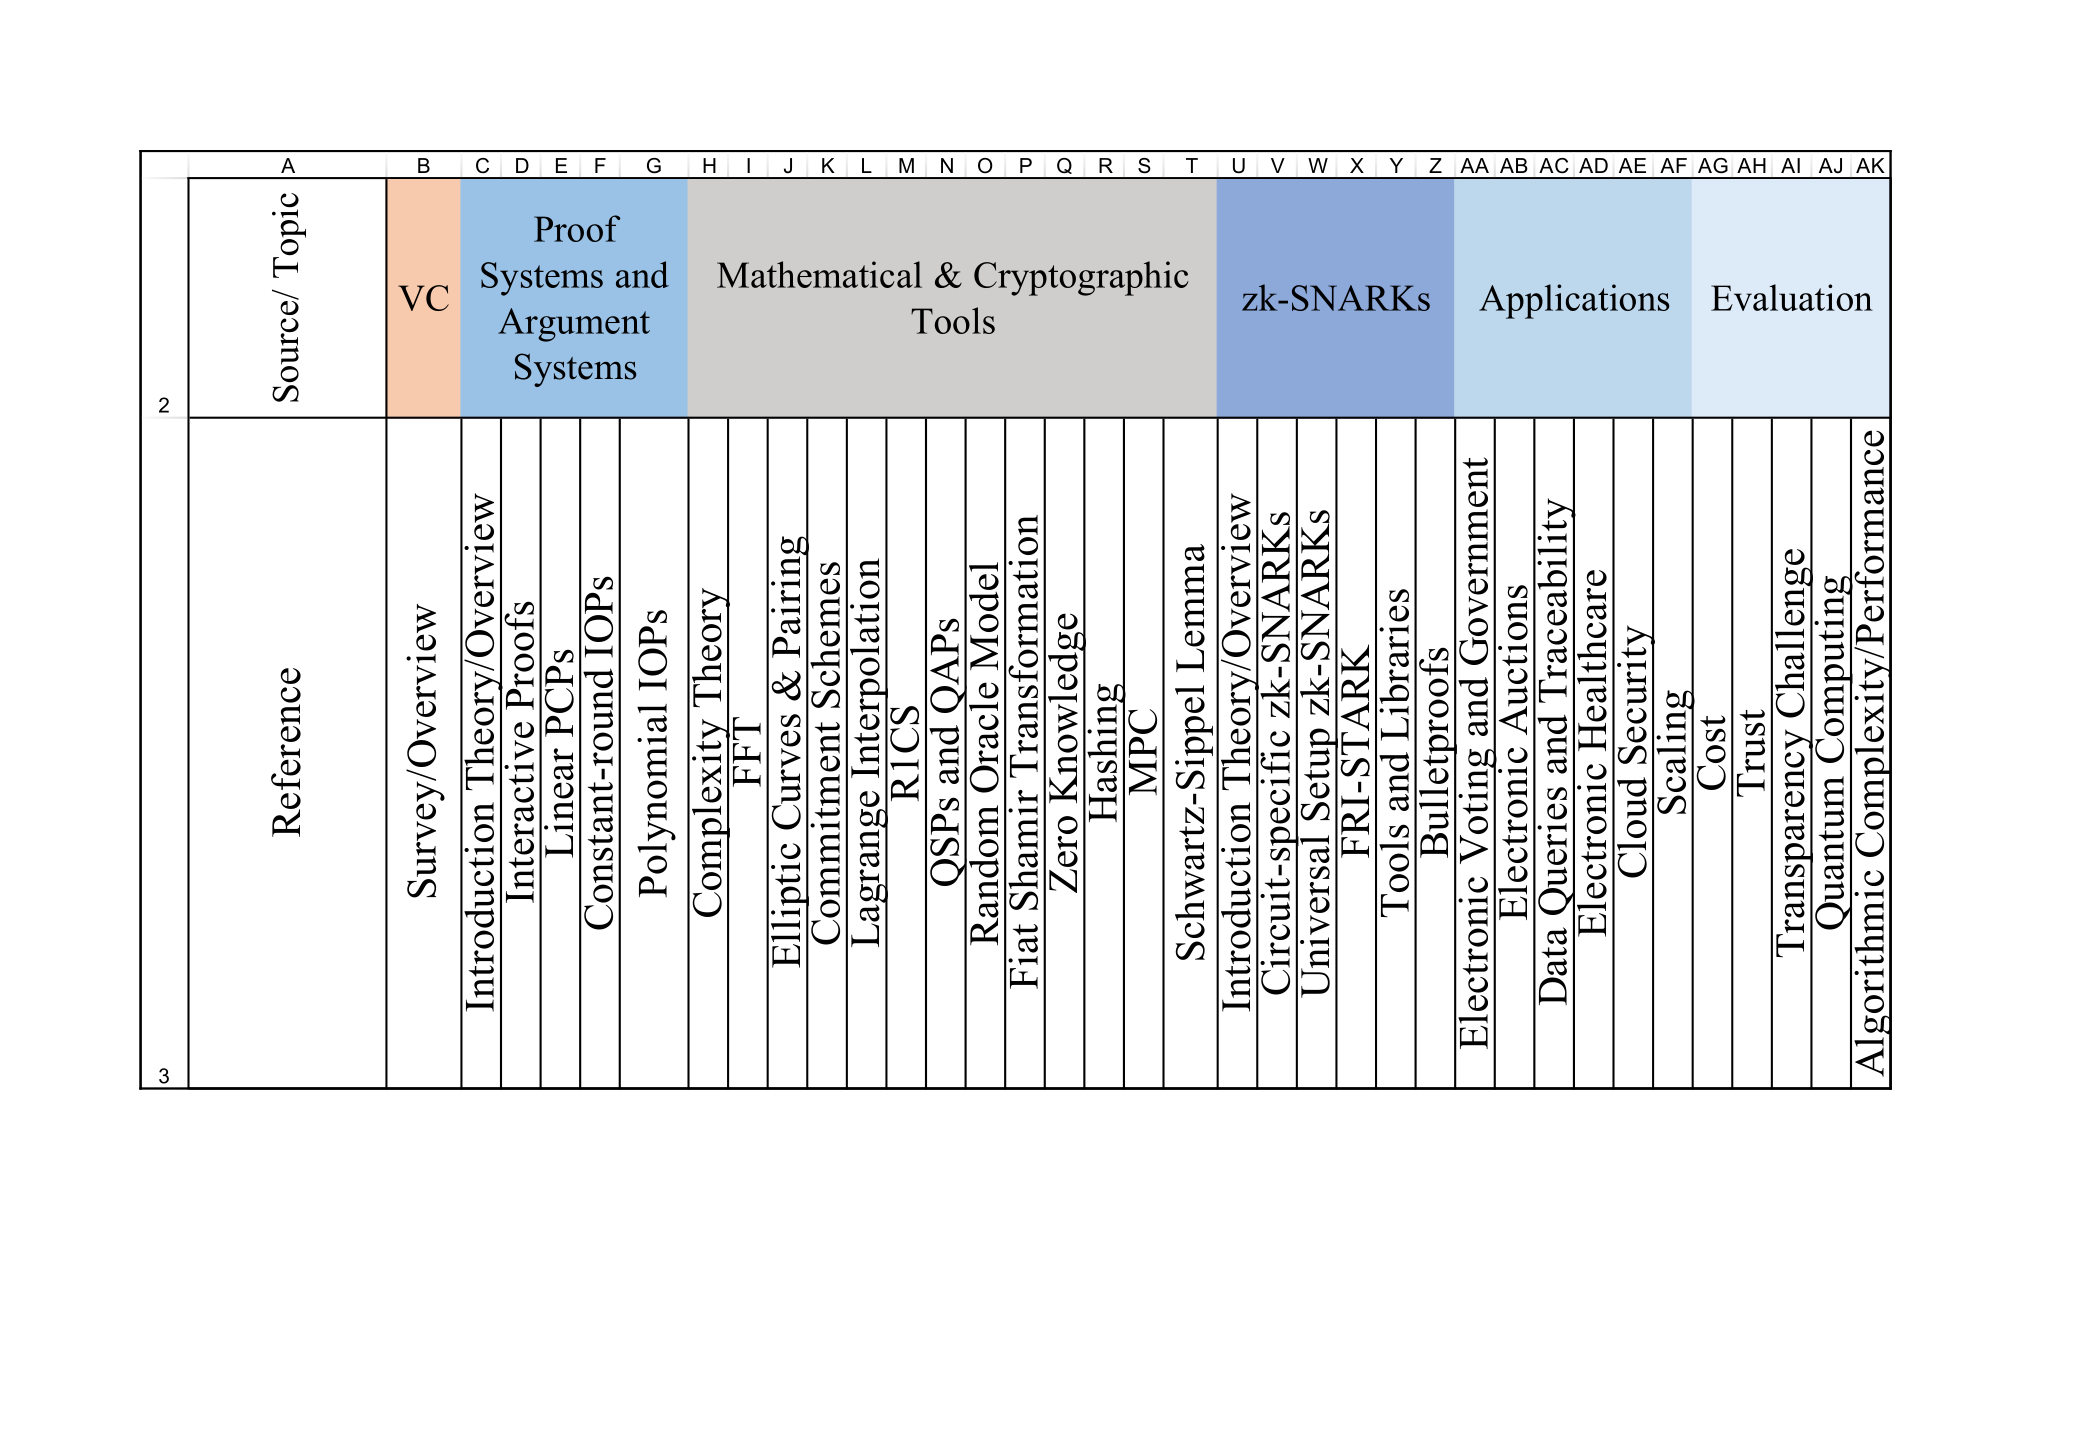
\includegraphics[width=1.0\textwidth]{Pictures/concept_matrix/wos-01.png}
\end{figure}

\begin{figure}[H]
	\centering
		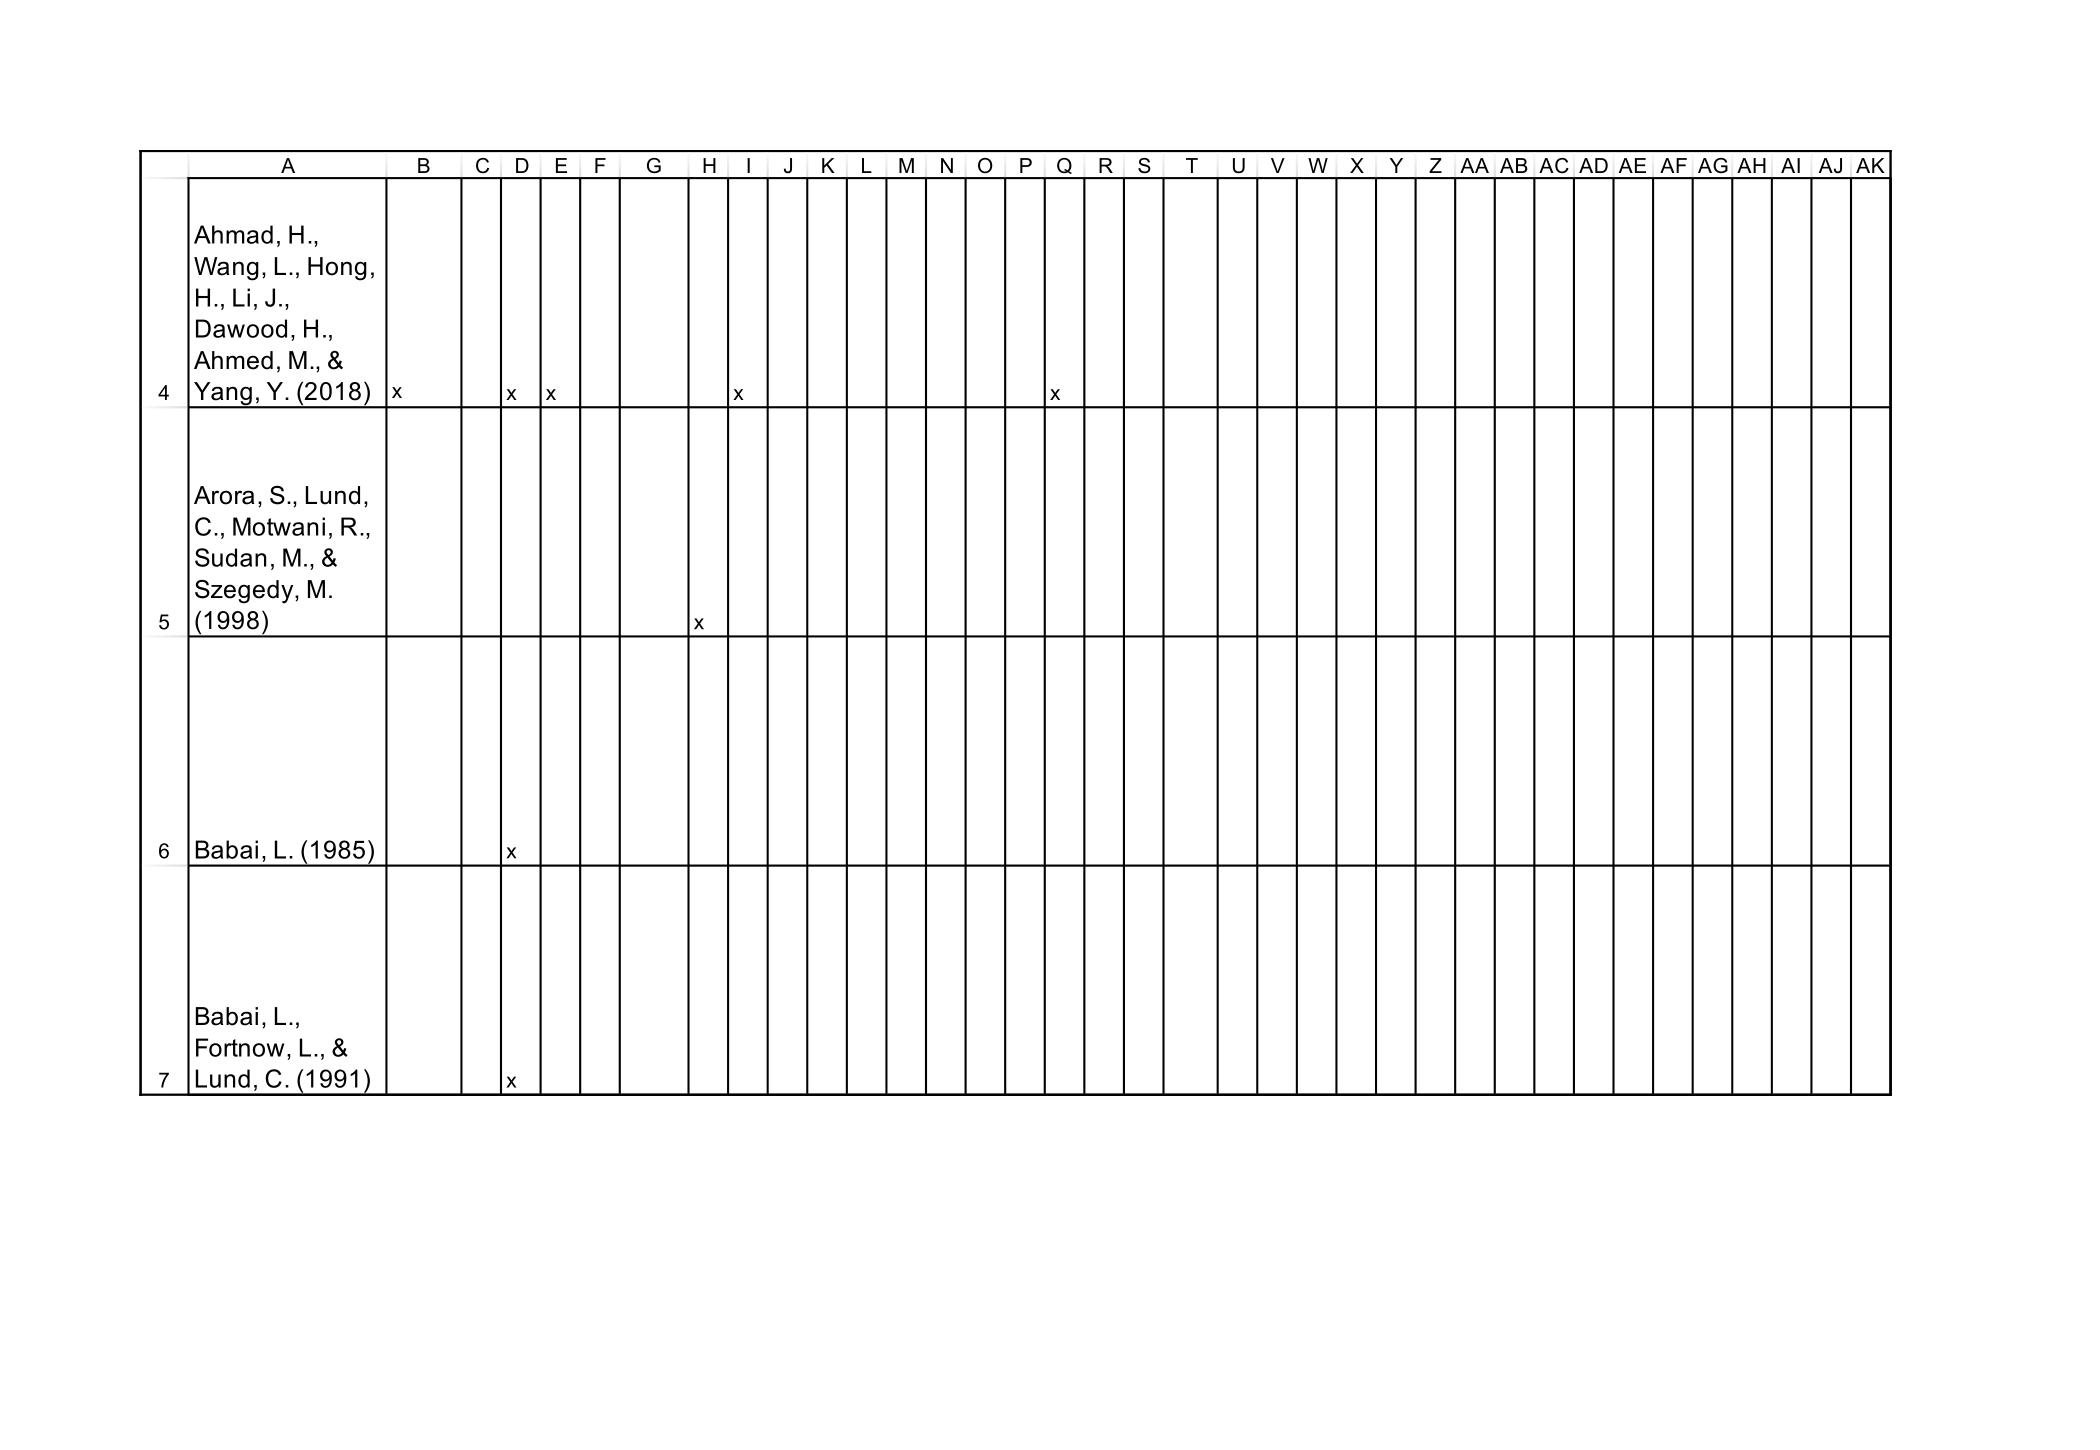
\includegraphics[width=.95\textwidth]{Pictures/concept_matrix/wos-02.png}
\end{figure}
\begin{figure}[H]
	\centering
		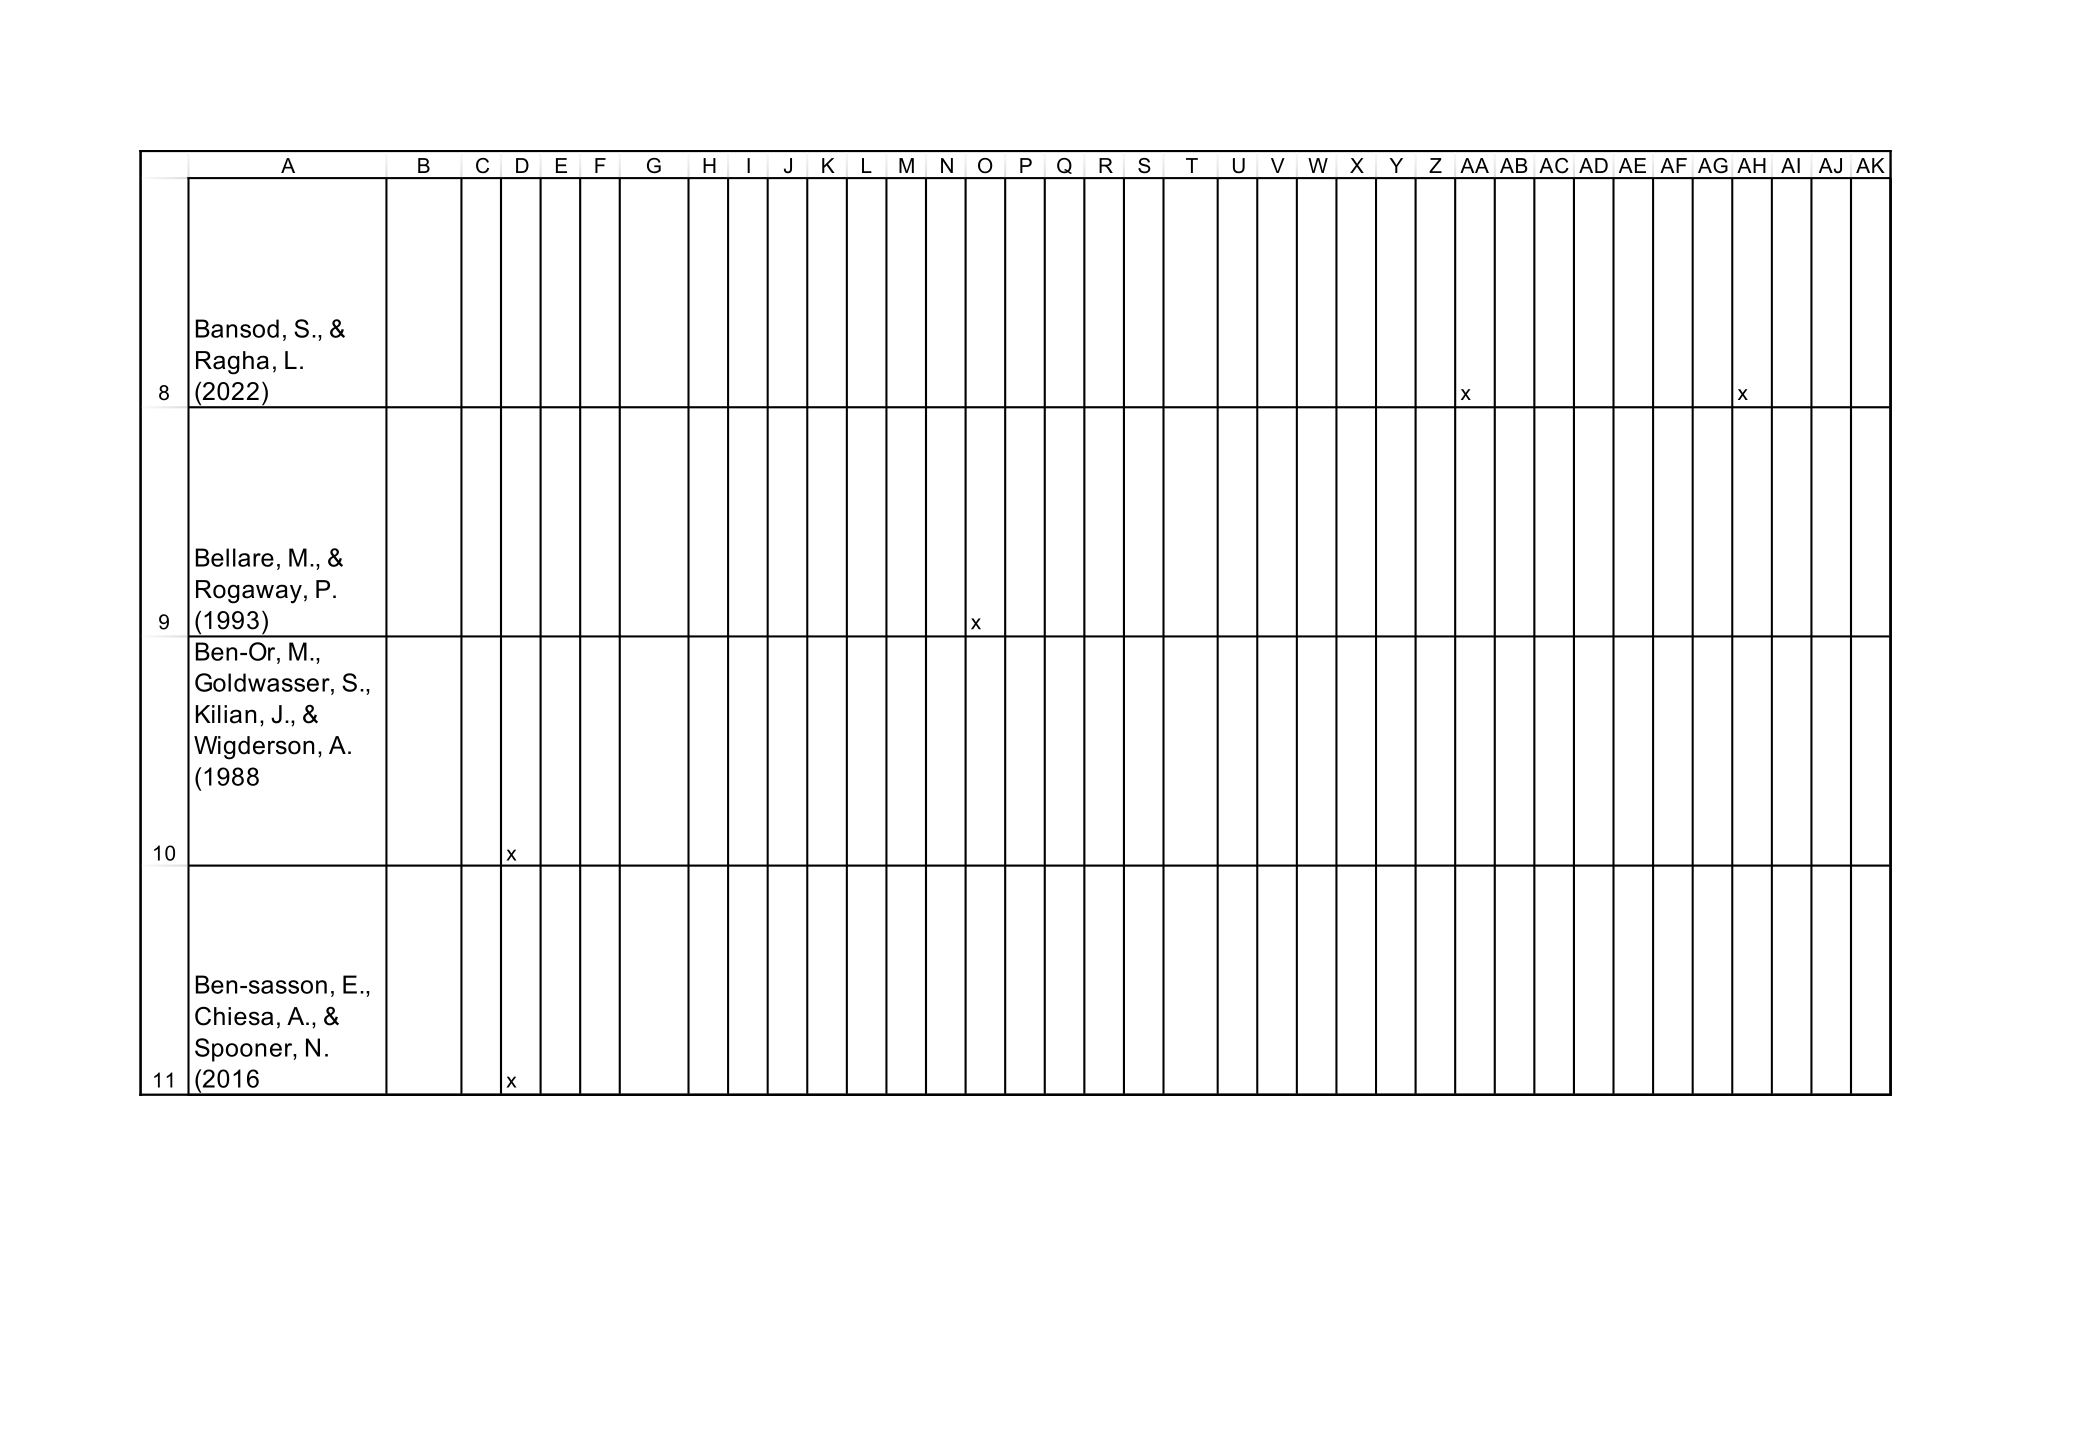
\includegraphics[width=.95\textwidth]{Pictures/concept_matrix/wos-03.png}
\end{figure}
\begin{figure}[H]
	\centering
		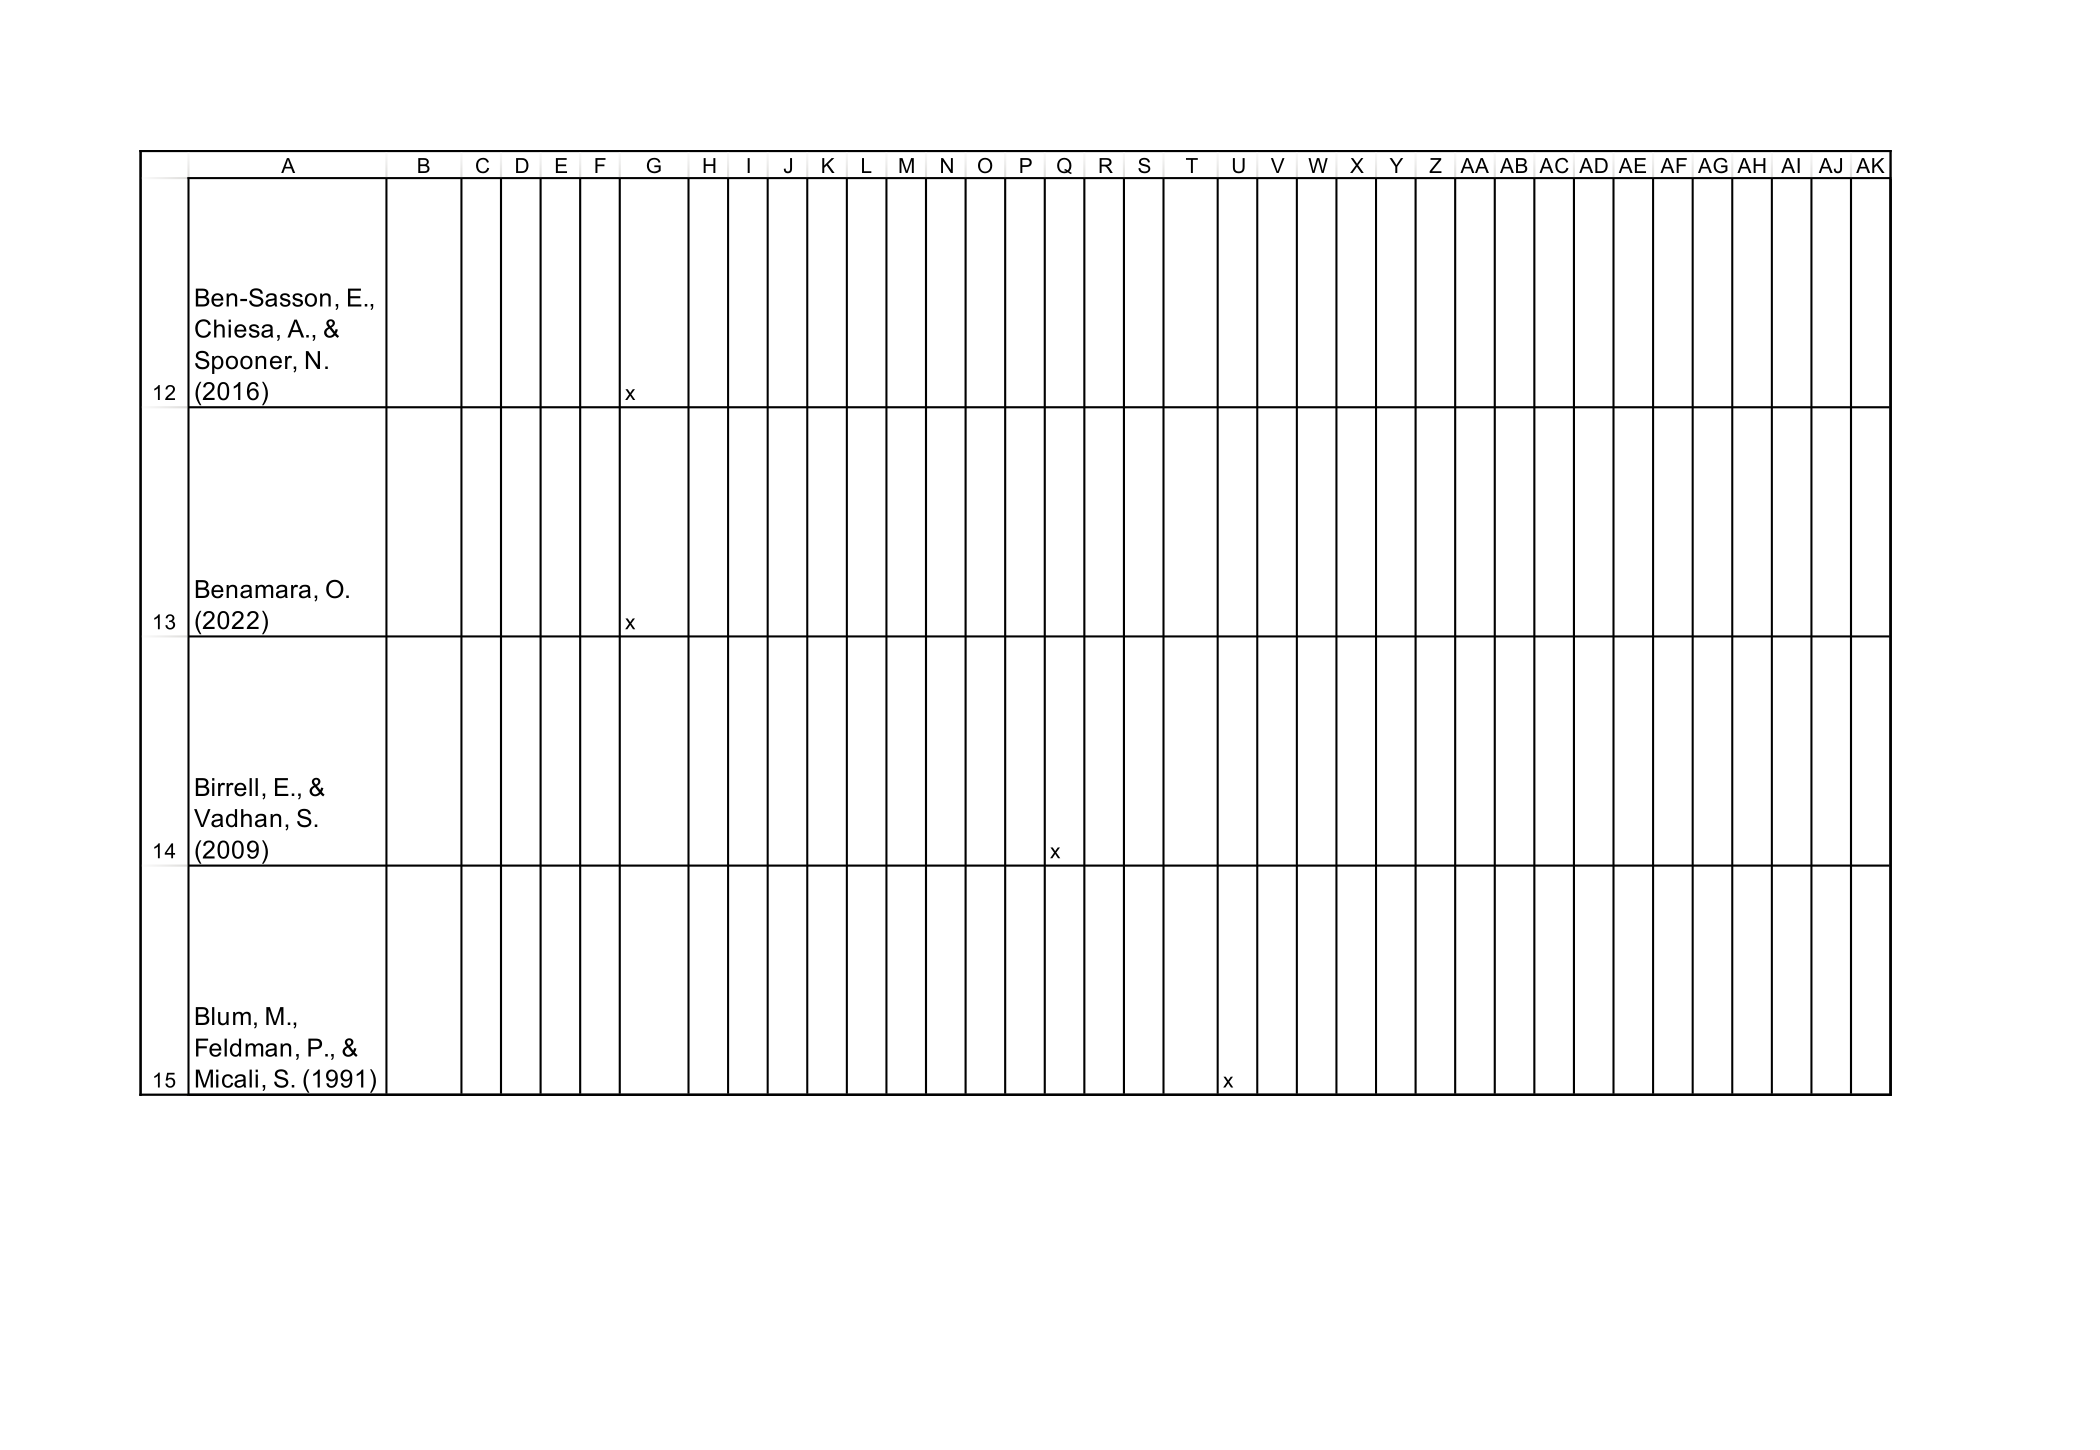
\includegraphics[width=.95\textwidth]{Pictures/concept_matrix/wos-04.png}
\end{figure}
\begin{figure}[H]
	\centering
		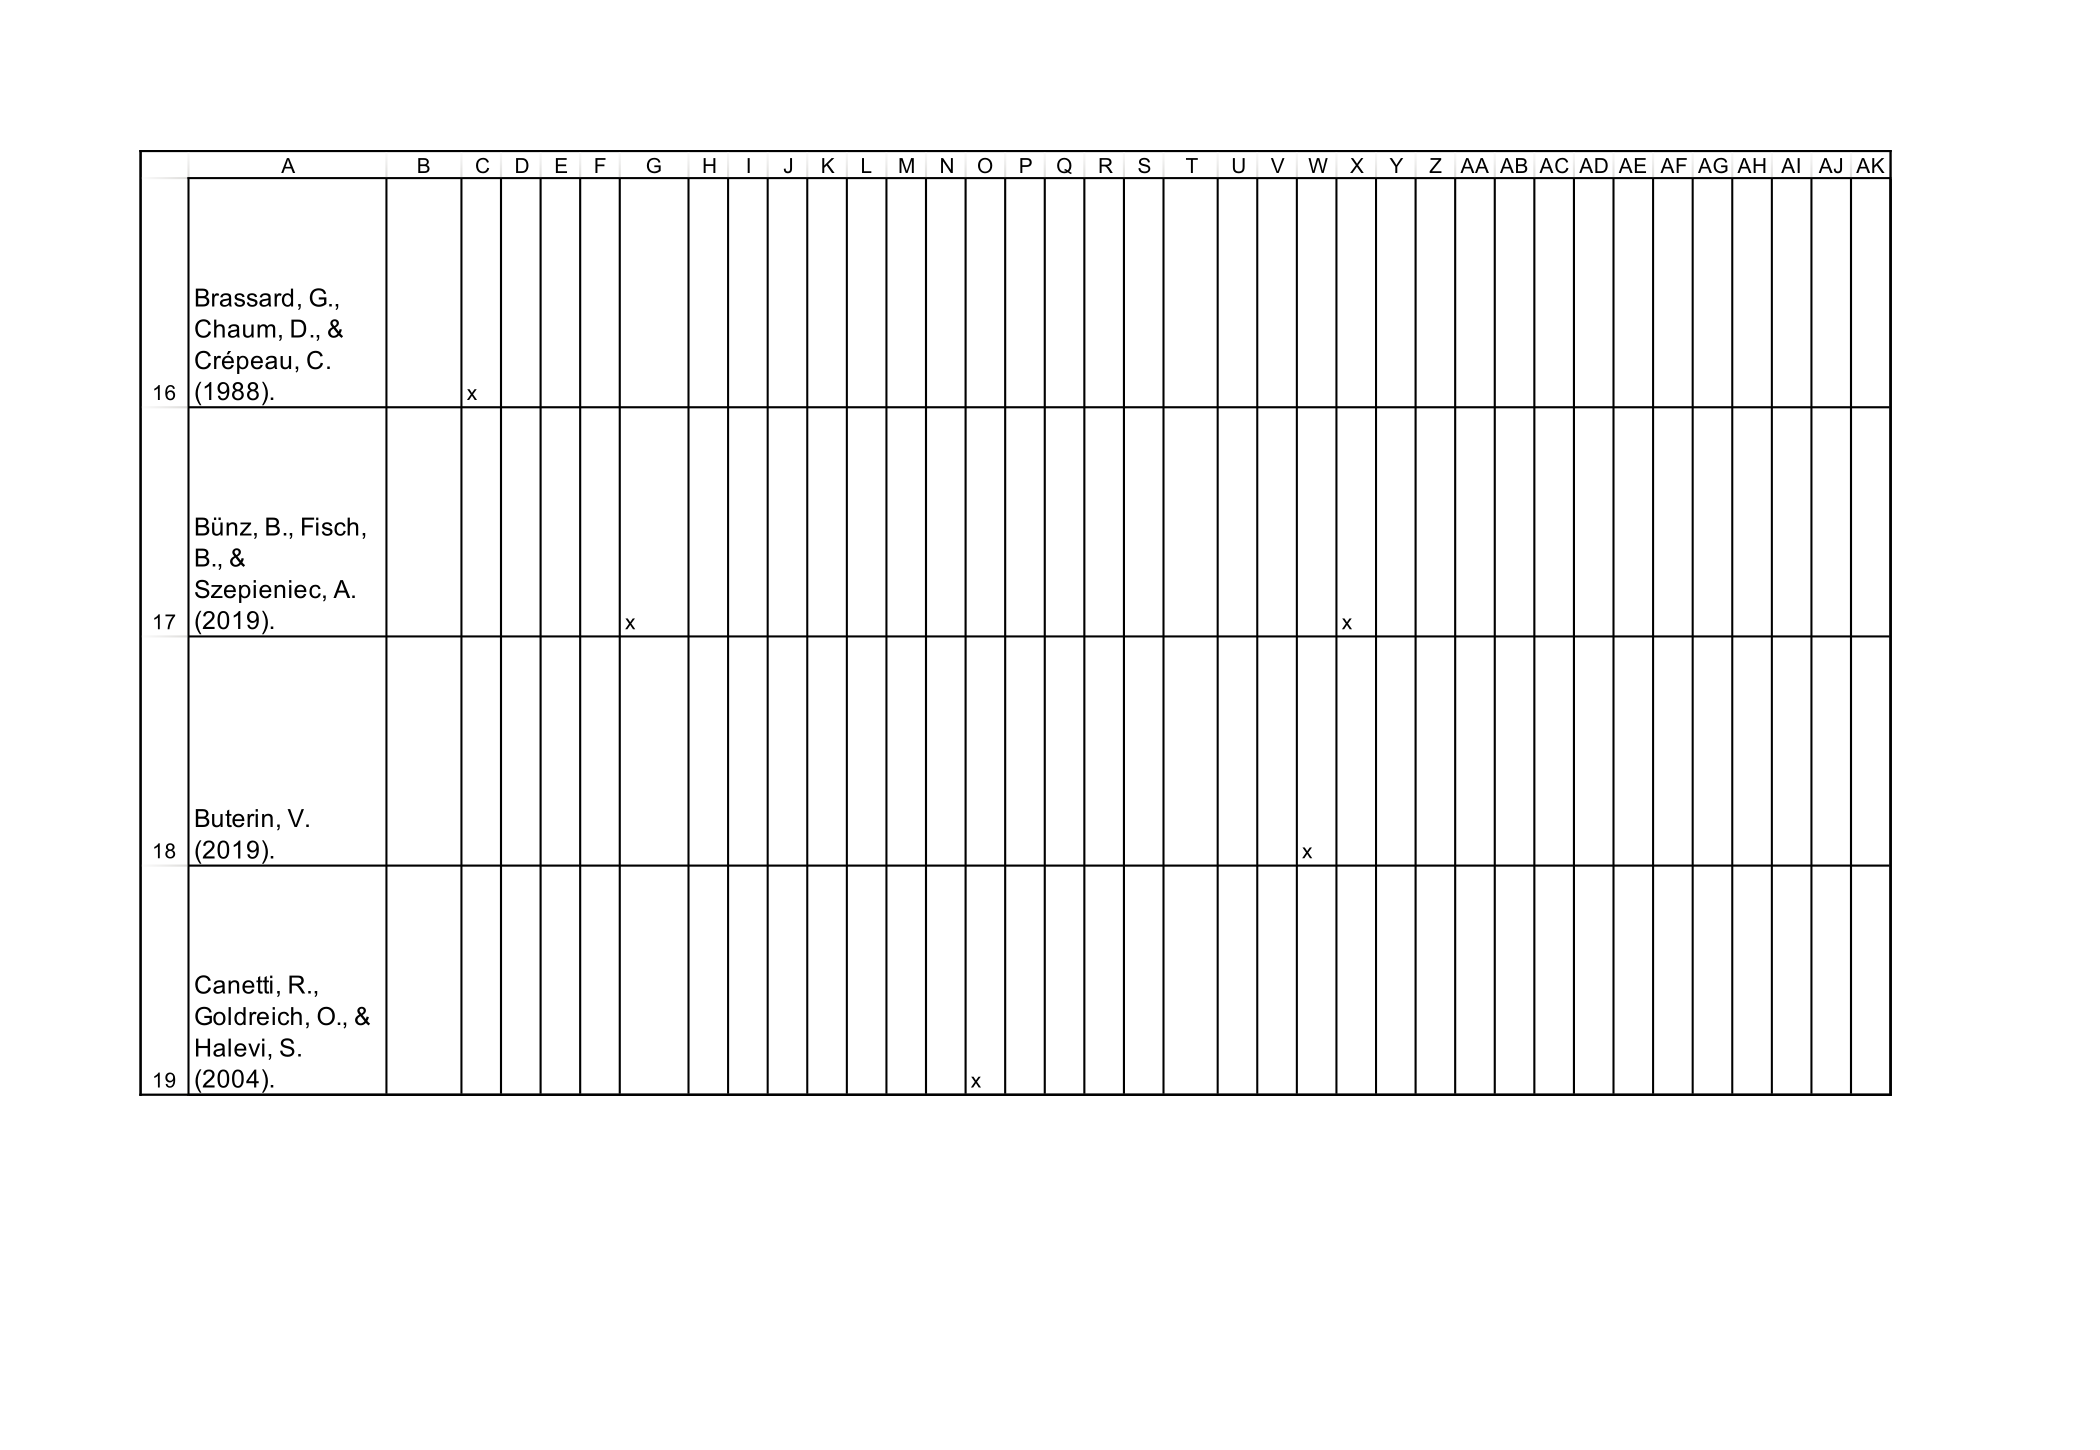
\includegraphics[width=.95\textwidth]{Pictures/concept_matrix/wos-05.png}
\end{figure}

\begin{figure}[H]
	\centering
		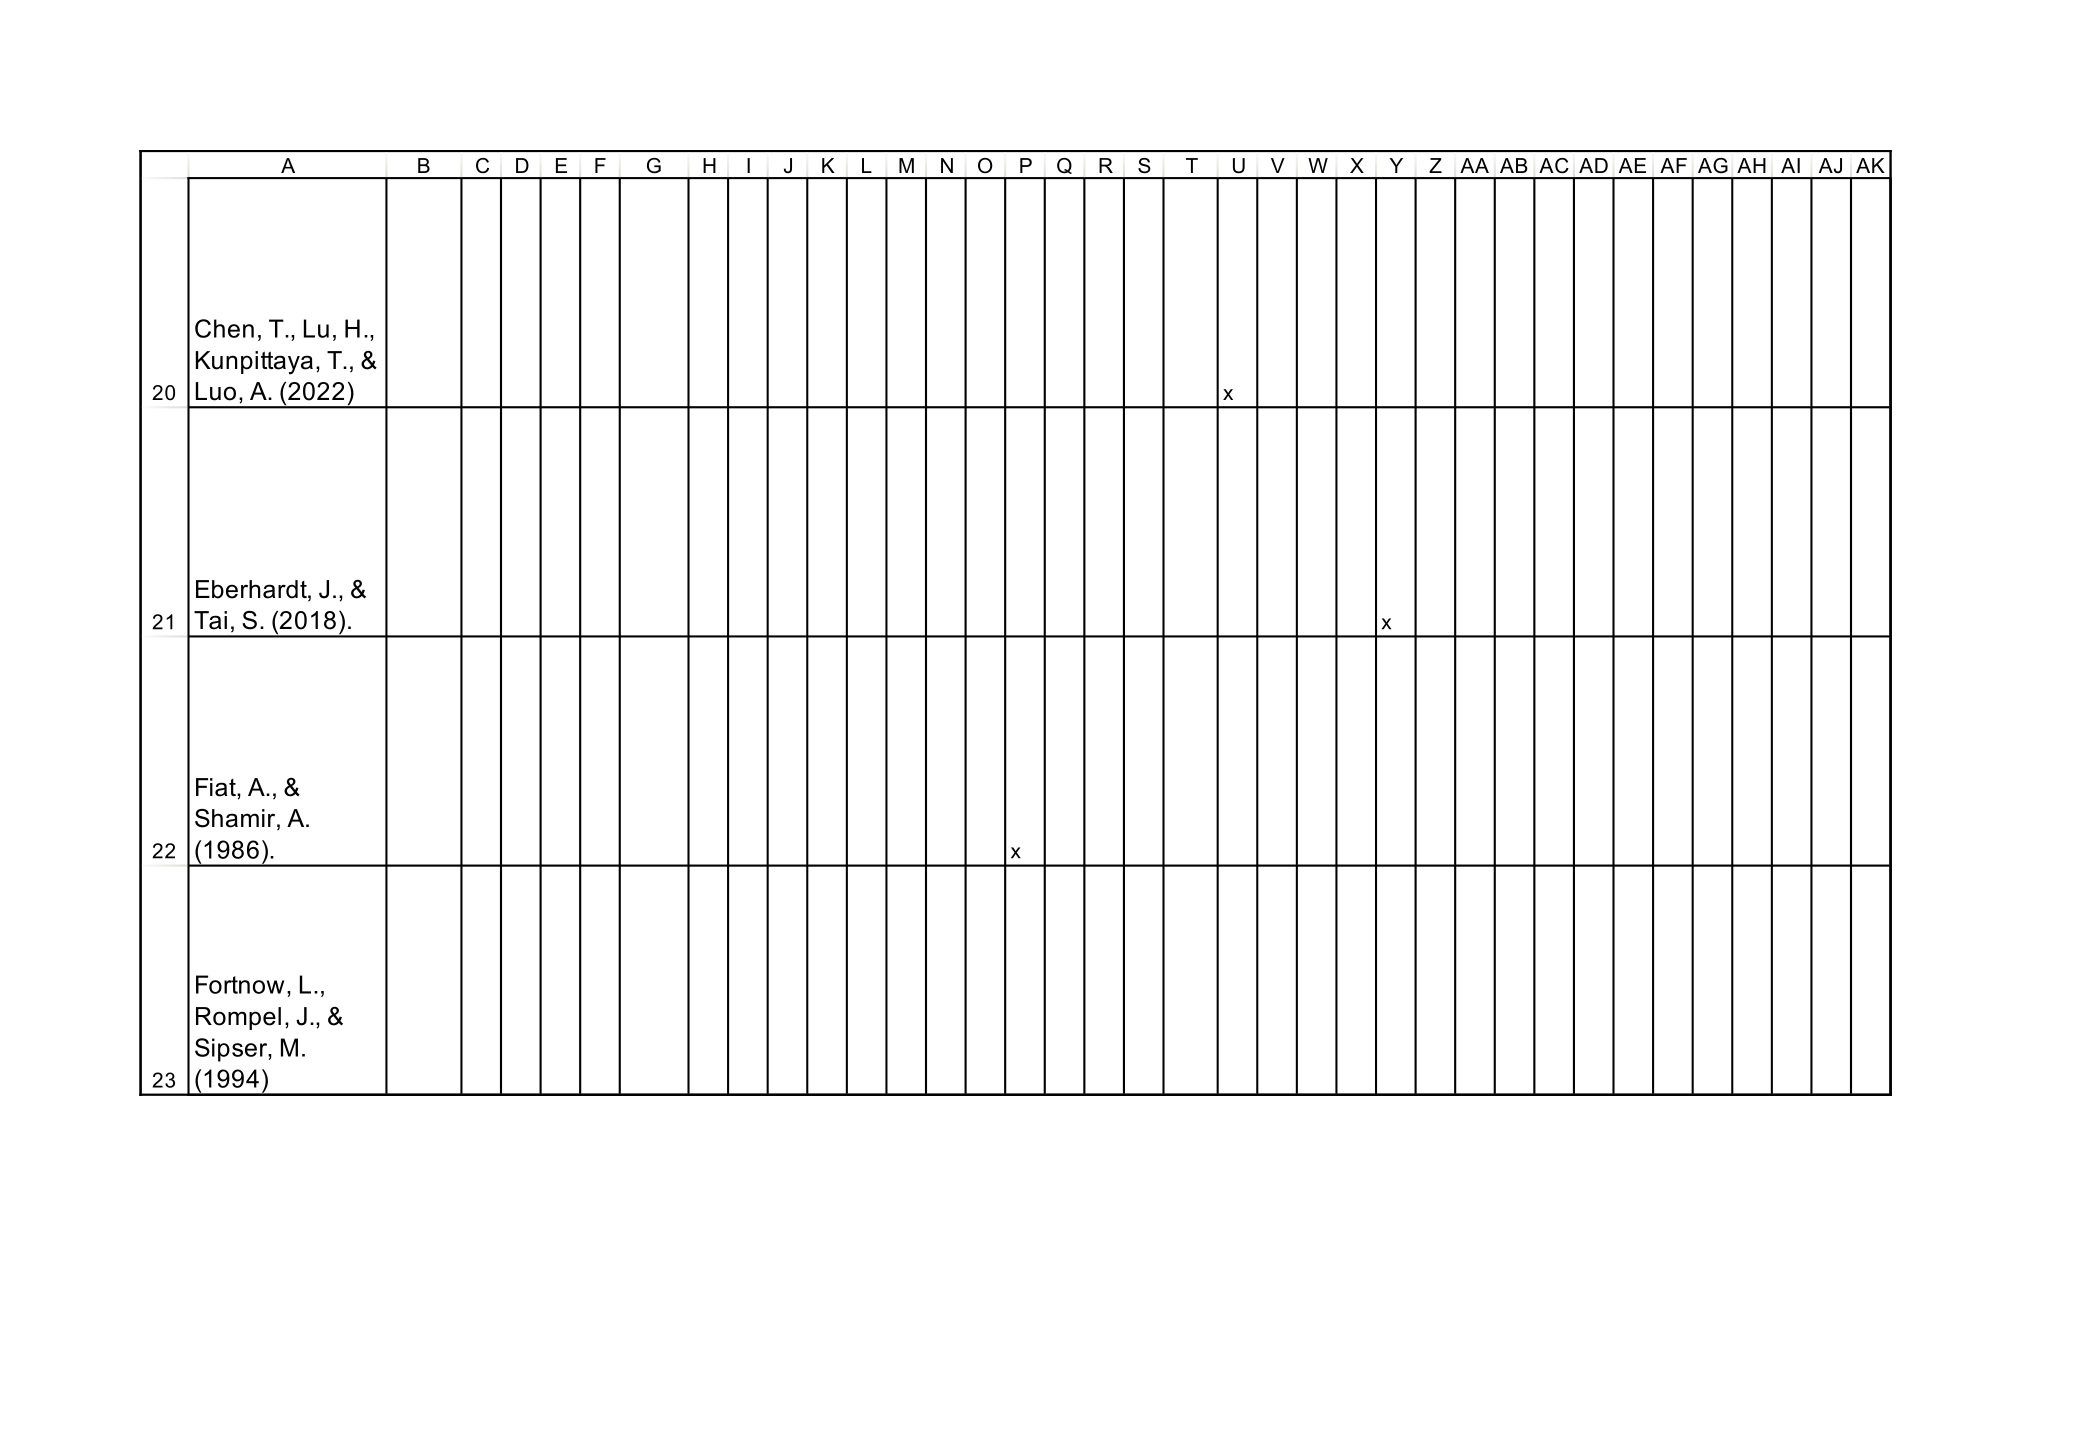
\includegraphics[width=.95\textwidth]{Pictures/concept_matrix/wos-06.png}
\end{figure}

\begin{figure}[H]
	\centering
		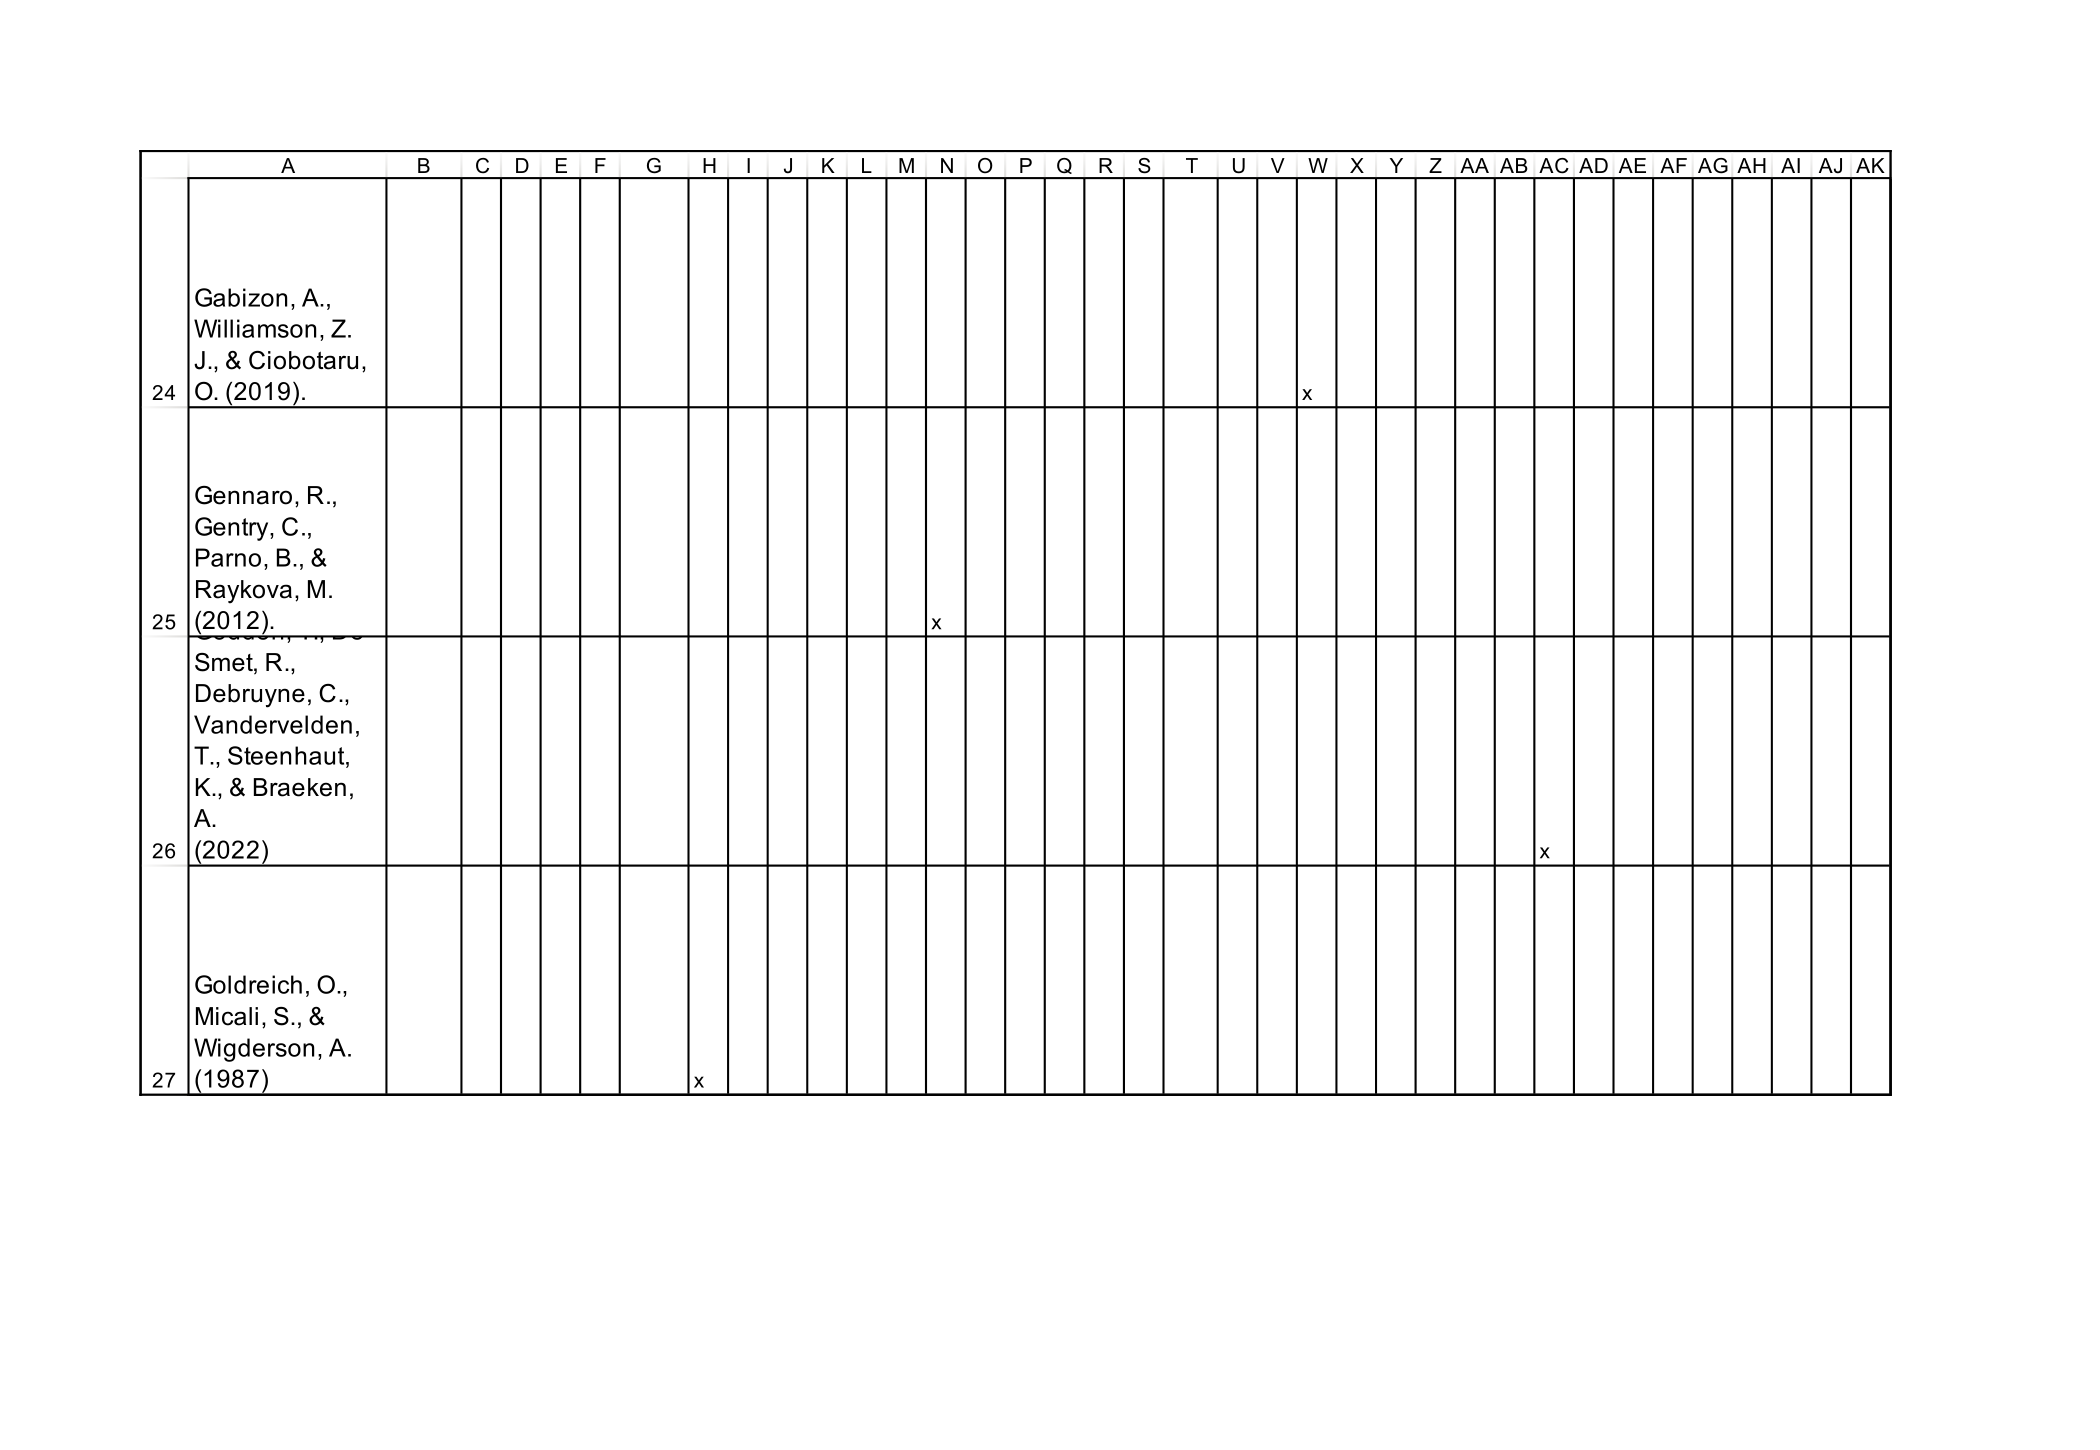
\includegraphics[width=.95\textwidth]{Pictures/concept_matrix/wos-07.png}
\end{figure}

\begin{figure}[H]
	\centering
		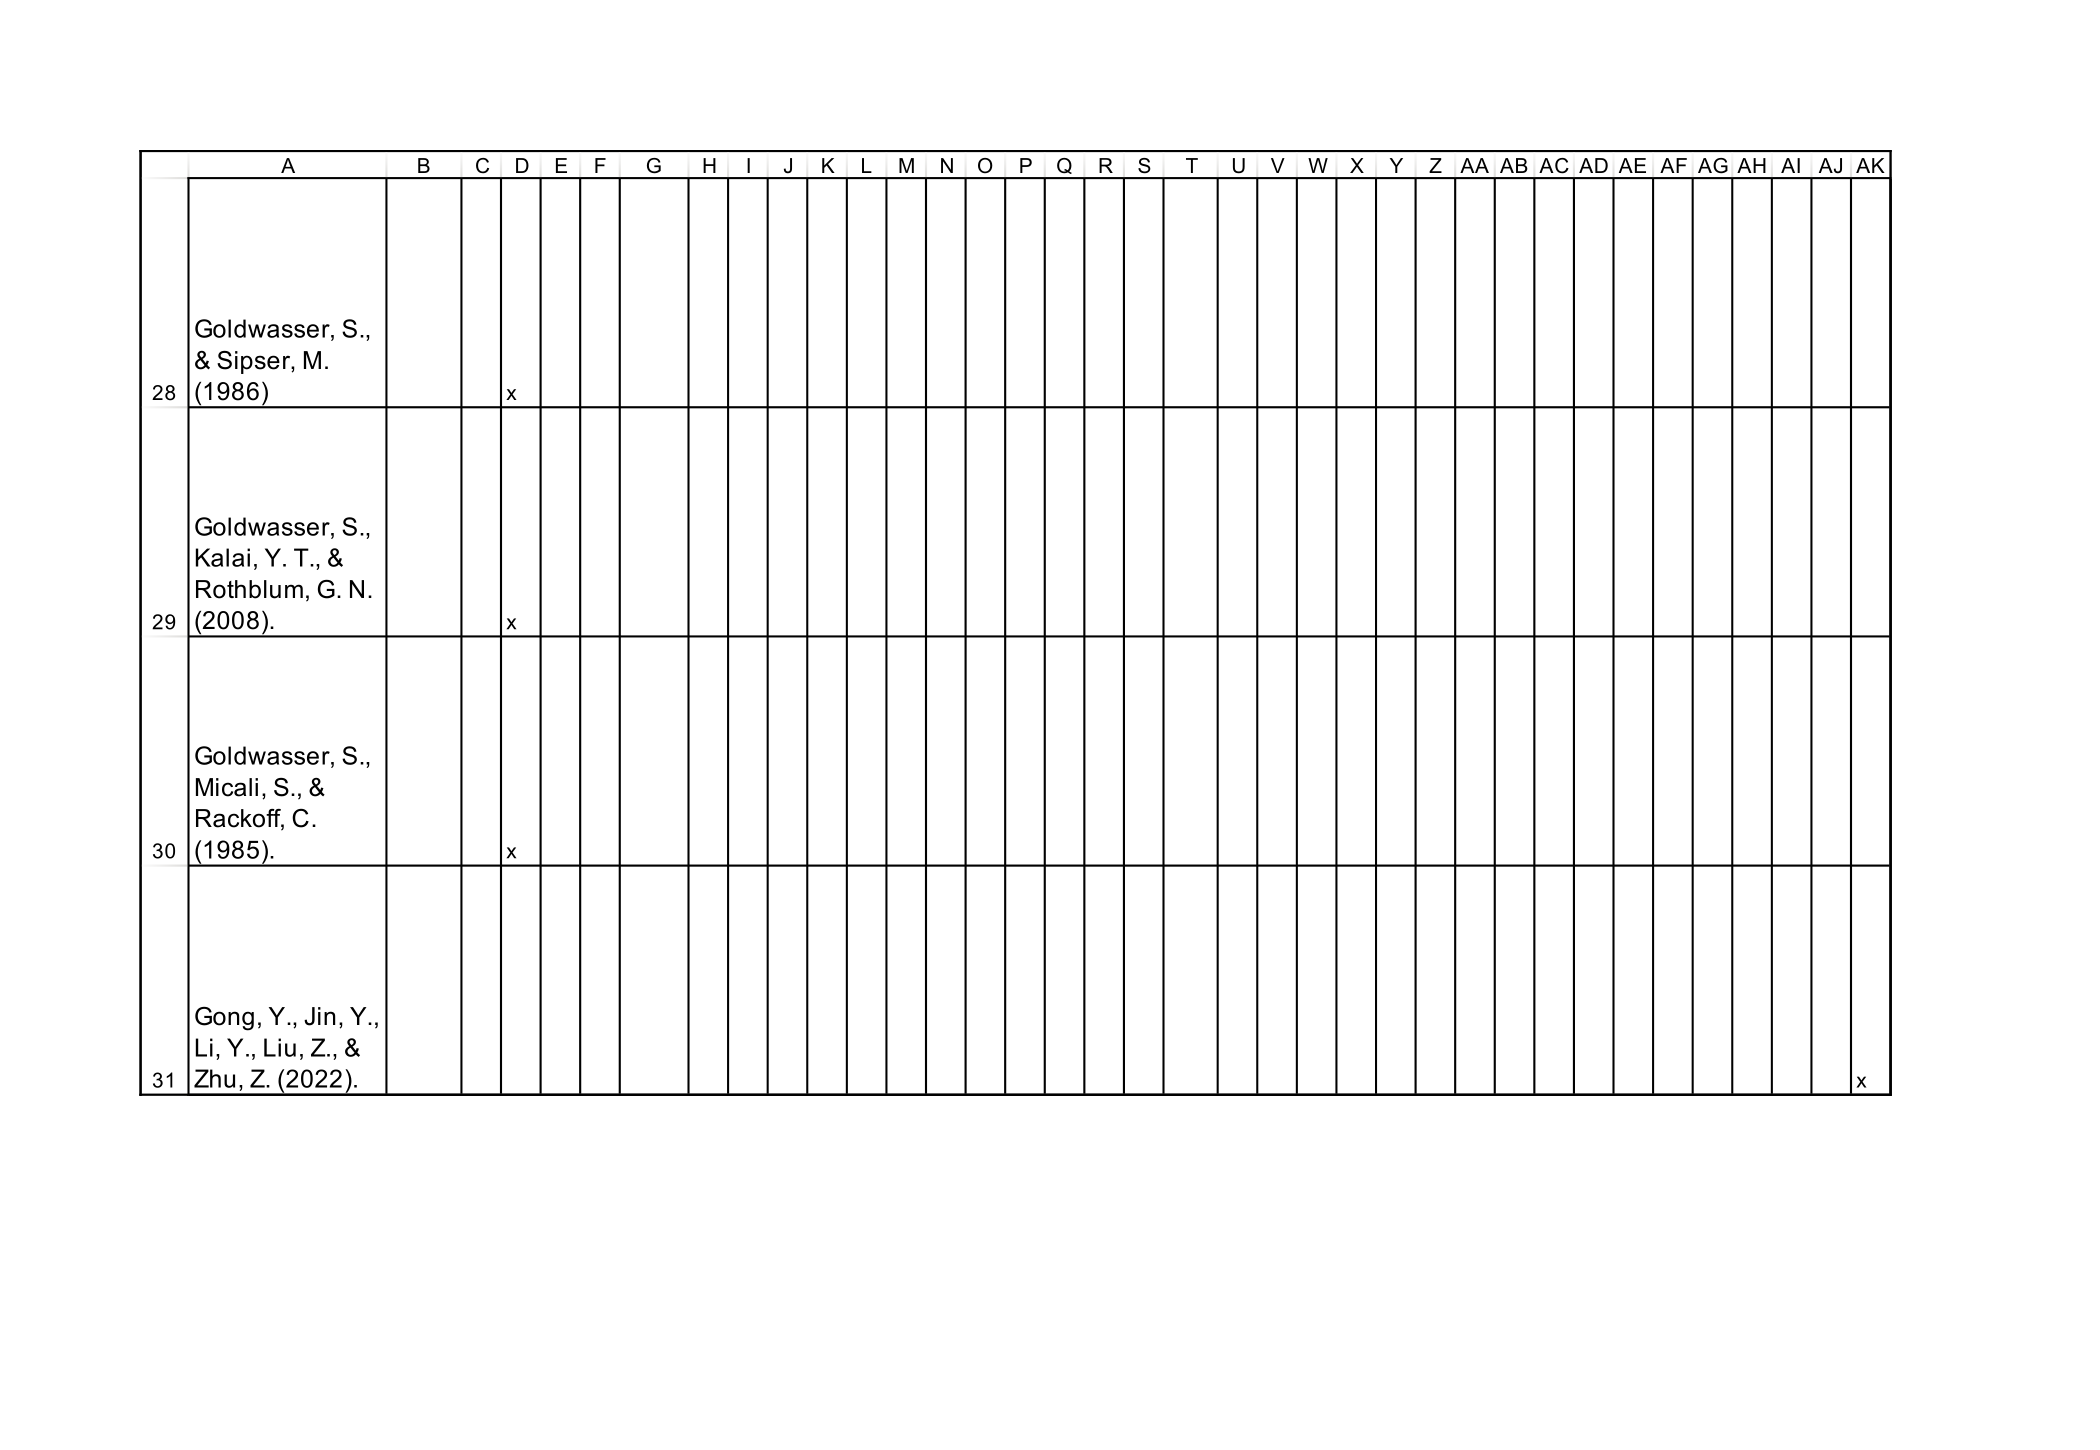
\includegraphics[width=.95\textwidth]{Pictures/concept_matrix/wos-08.png}
\end{figure}

\begin{figure}[H]
	\centering
		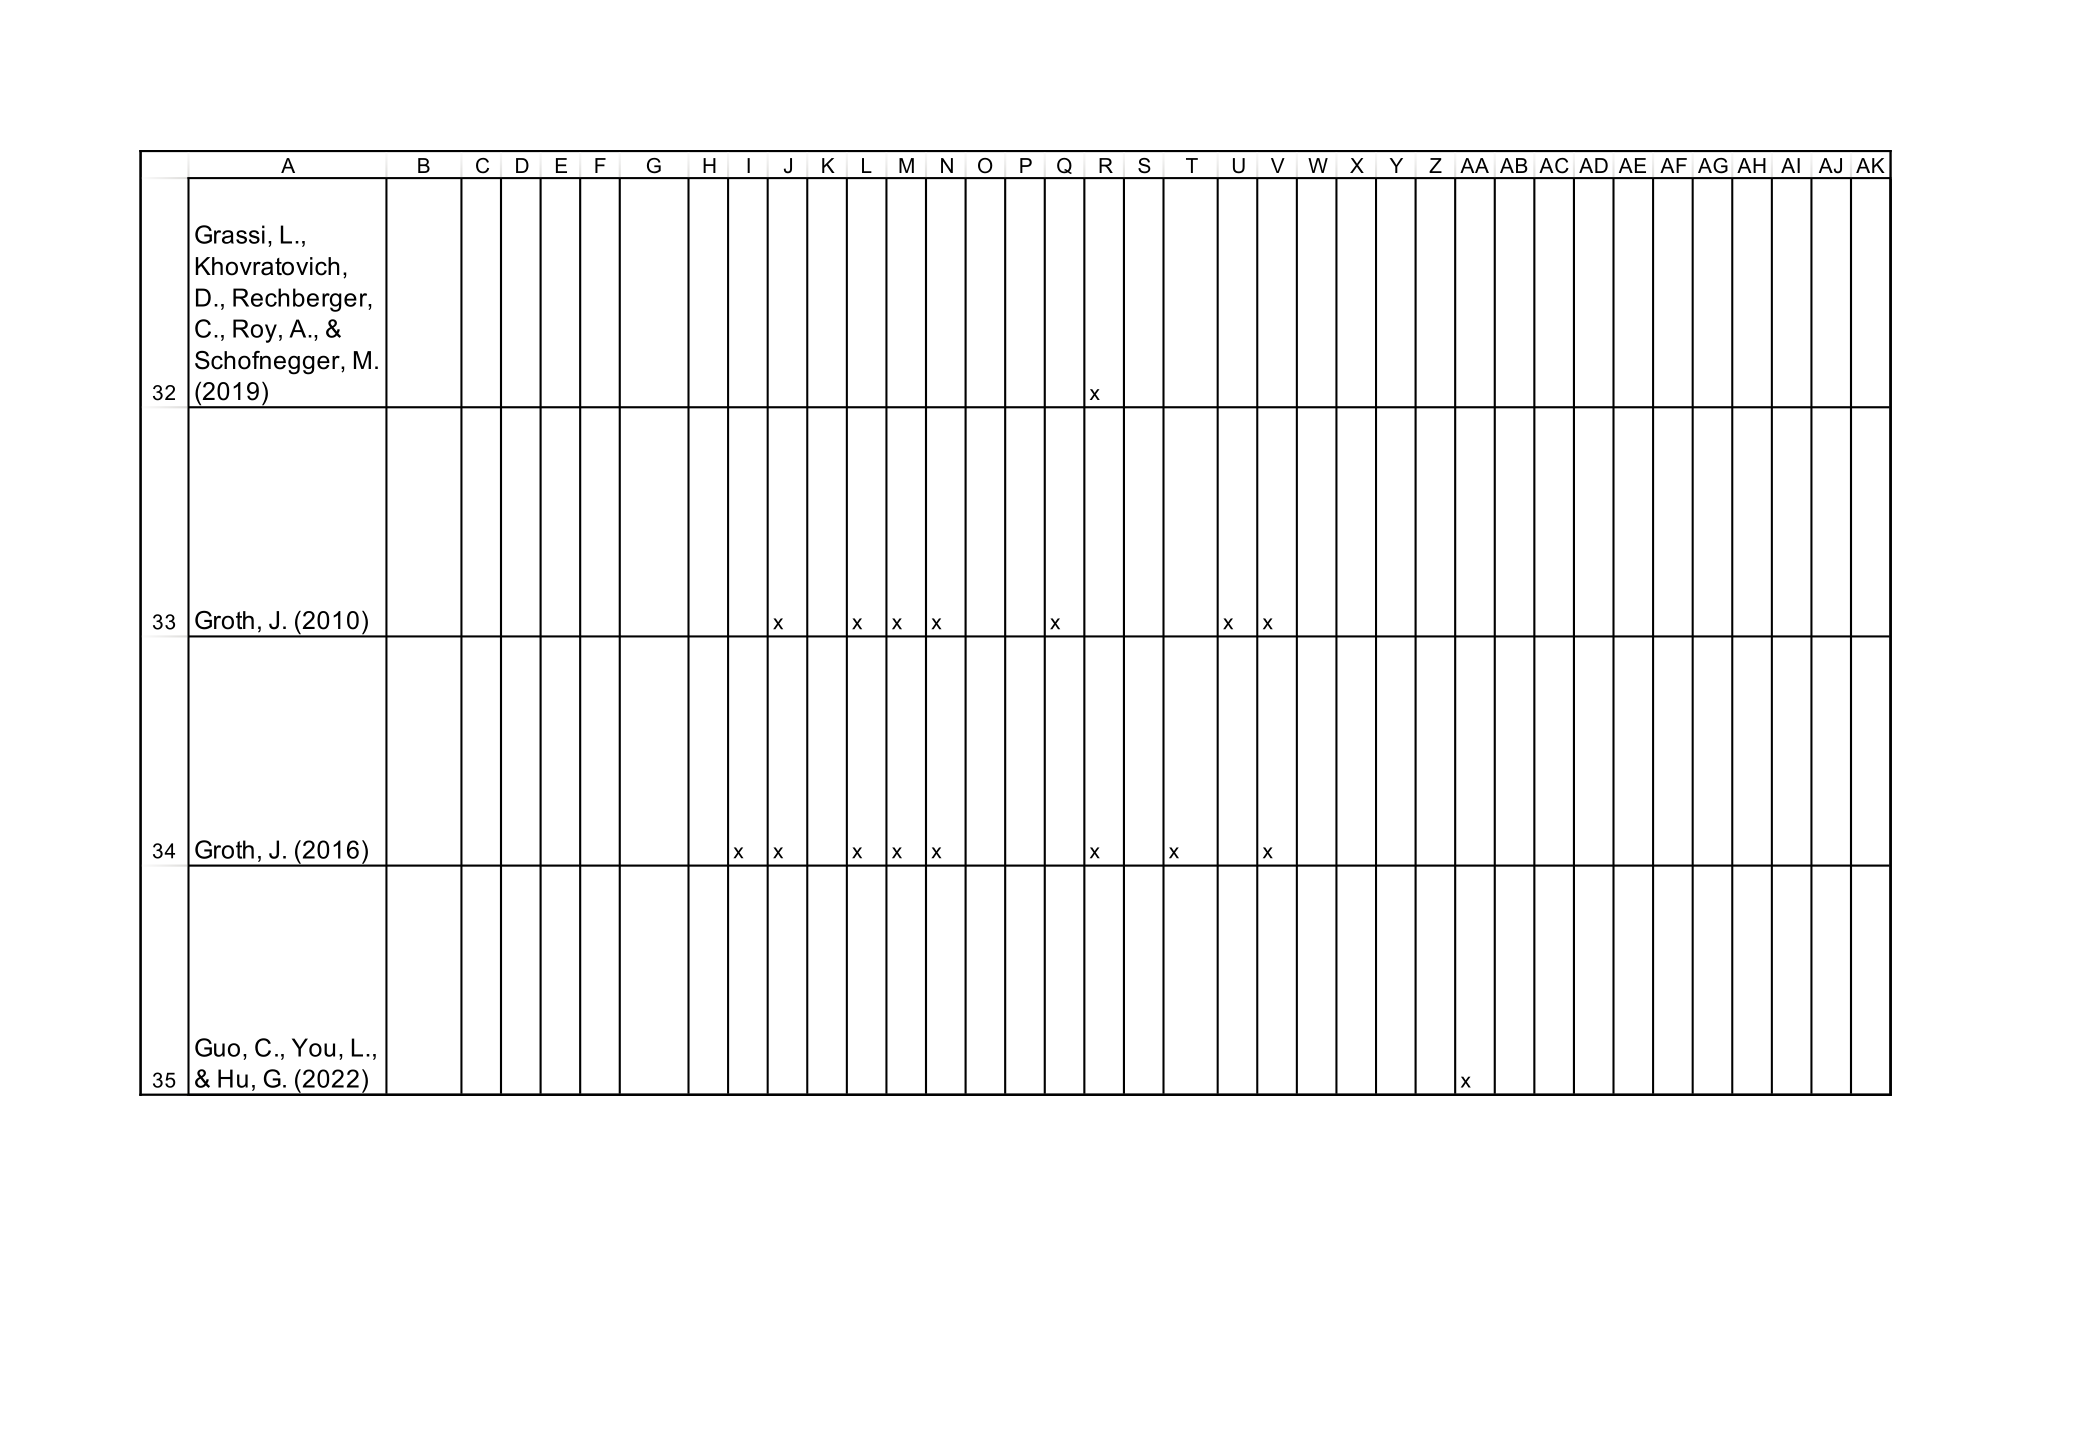
\includegraphics[width=.95\textwidth]{Pictures/concept_matrix/wos-09.png}
\end{figure}

\begin{figure}[H]
	\centering
		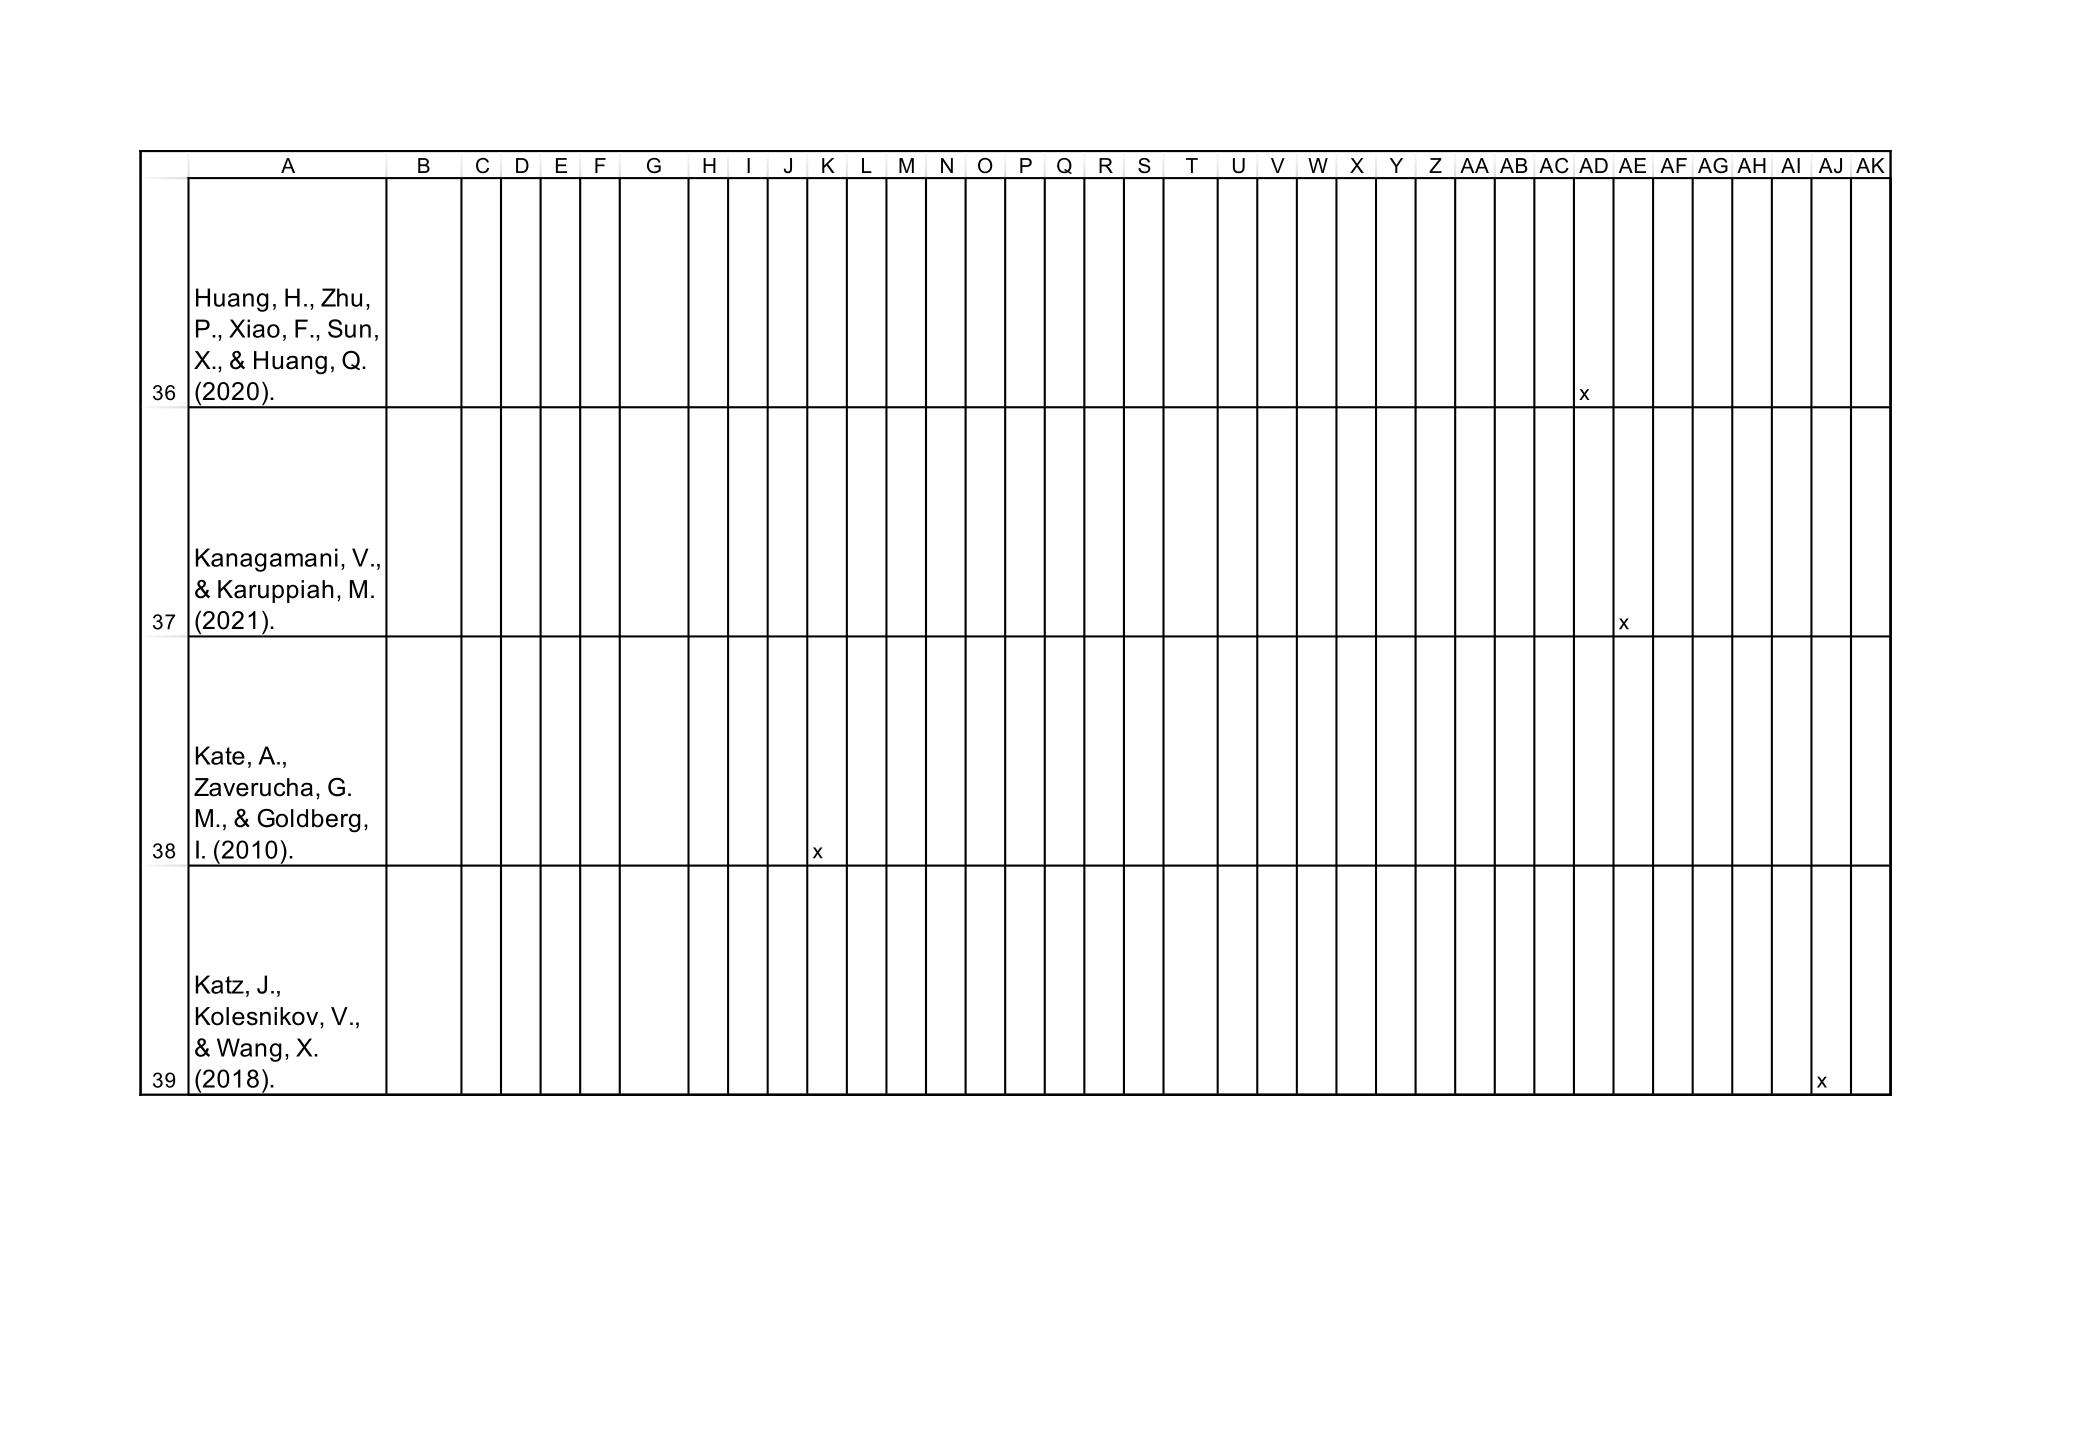
\includegraphics[width=.95\textwidth]{Pictures/concept_matrix/wos-10.png}
\end{figure}

\begin{figure}[H]
	\centering
		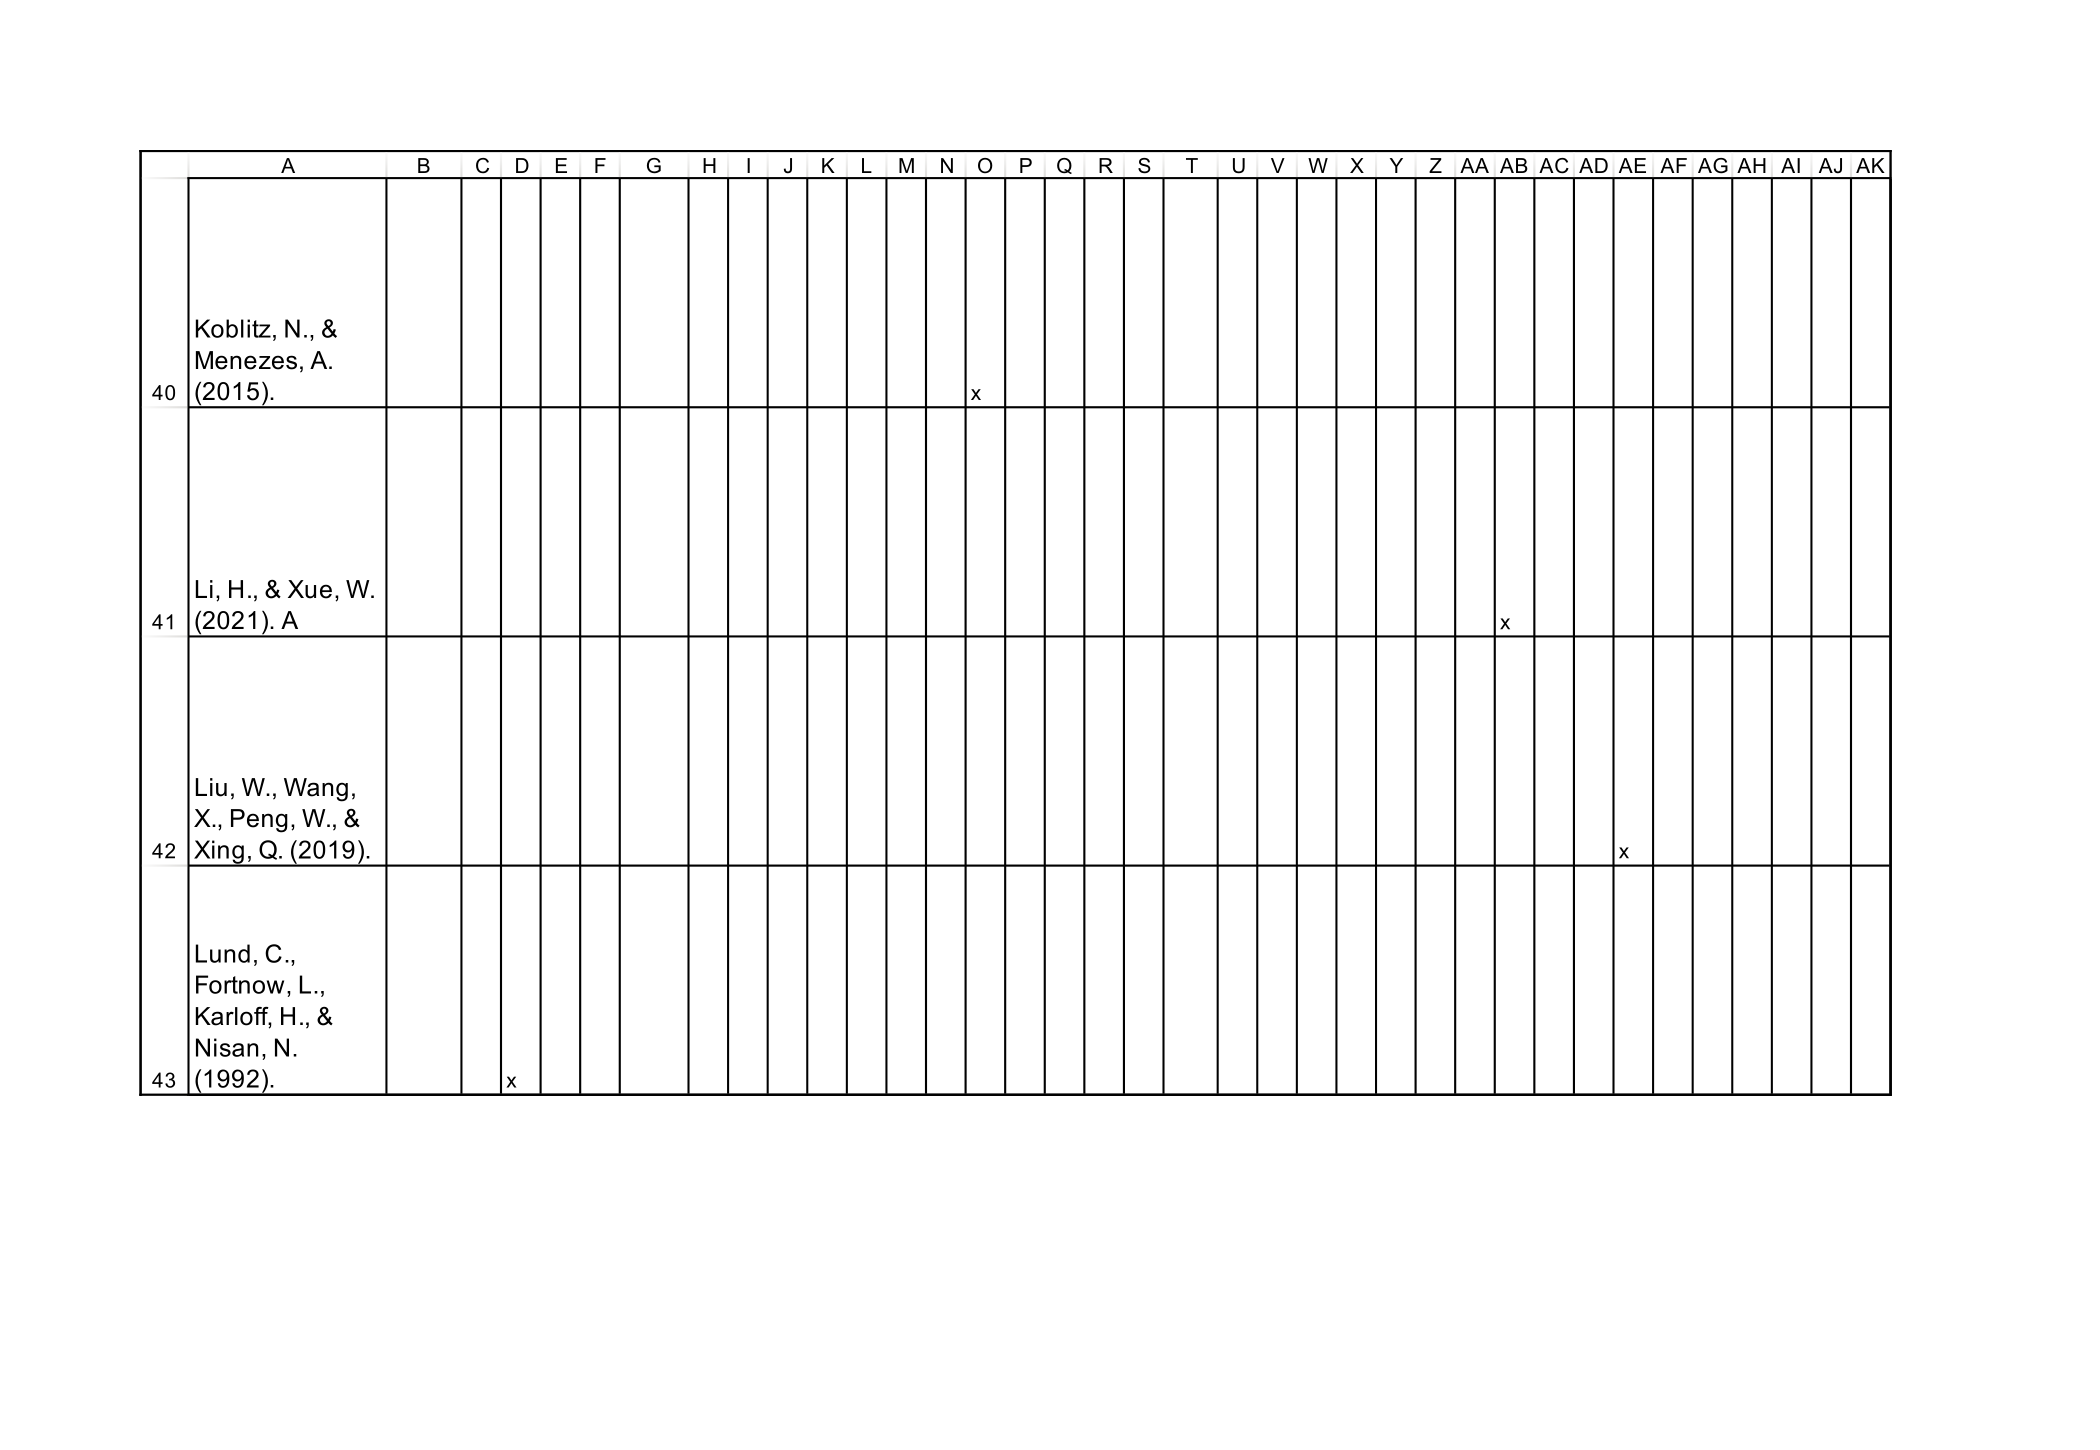
\includegraphics[width=.95\textwidth]{Pictures/concept_matrix/wos-11.png}
\end{figure}

\begin{figure}[H]
	\centering
		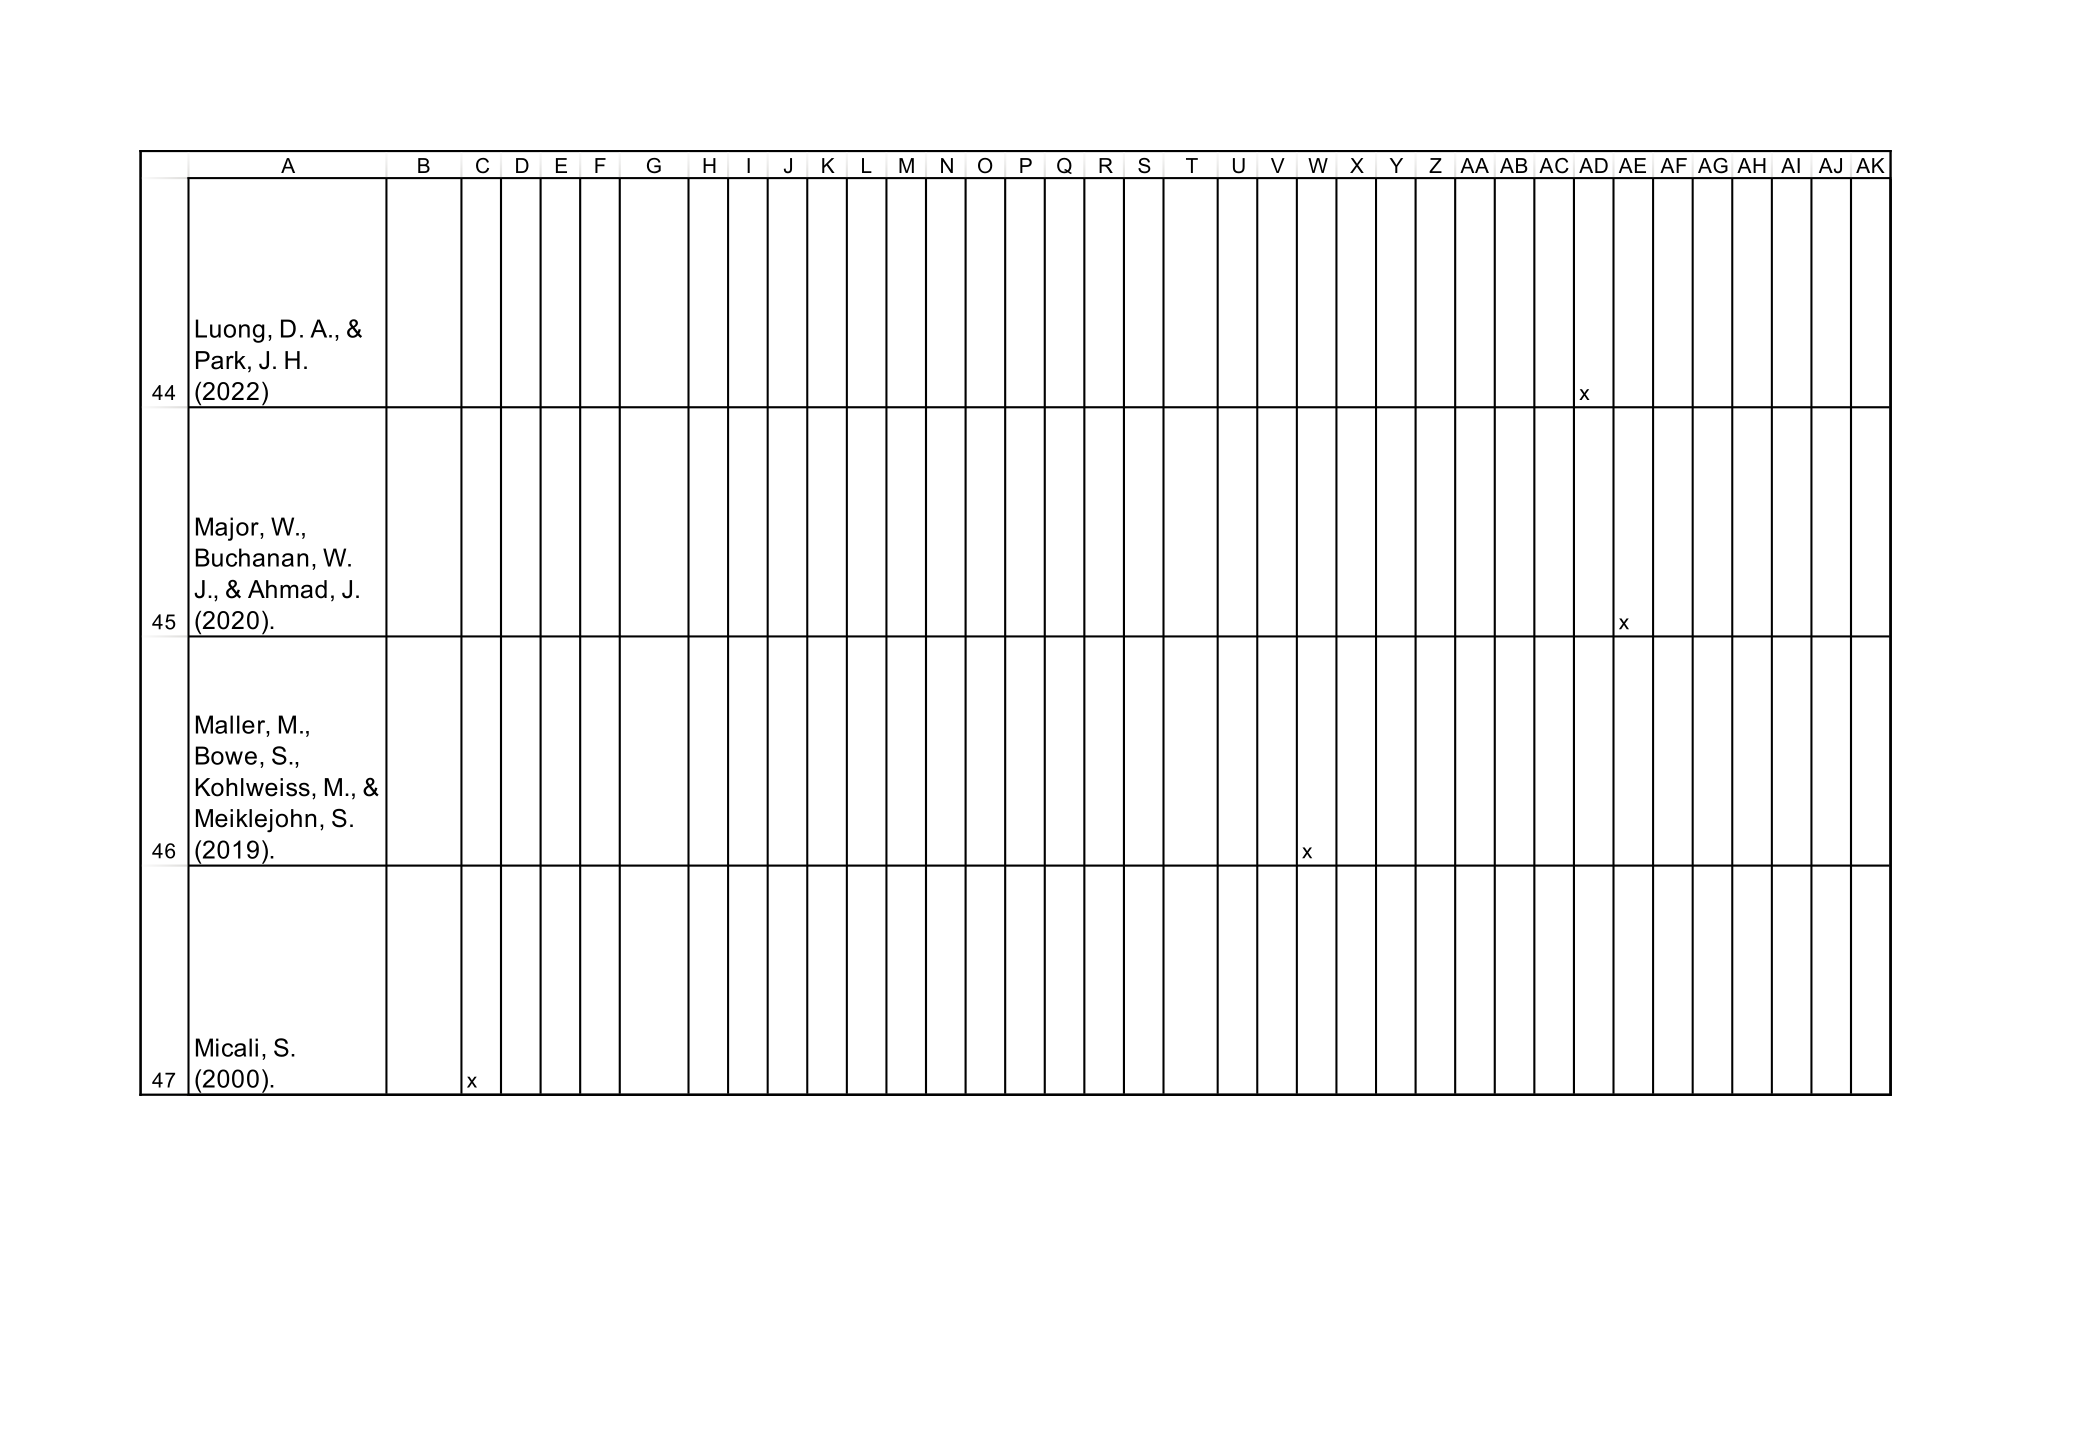
\includegraphics[width=.95\textwidth]{Pictures/concept_matrix/wos-12.png}
\end{figure}

\begin{figure}[H]
	\centering
		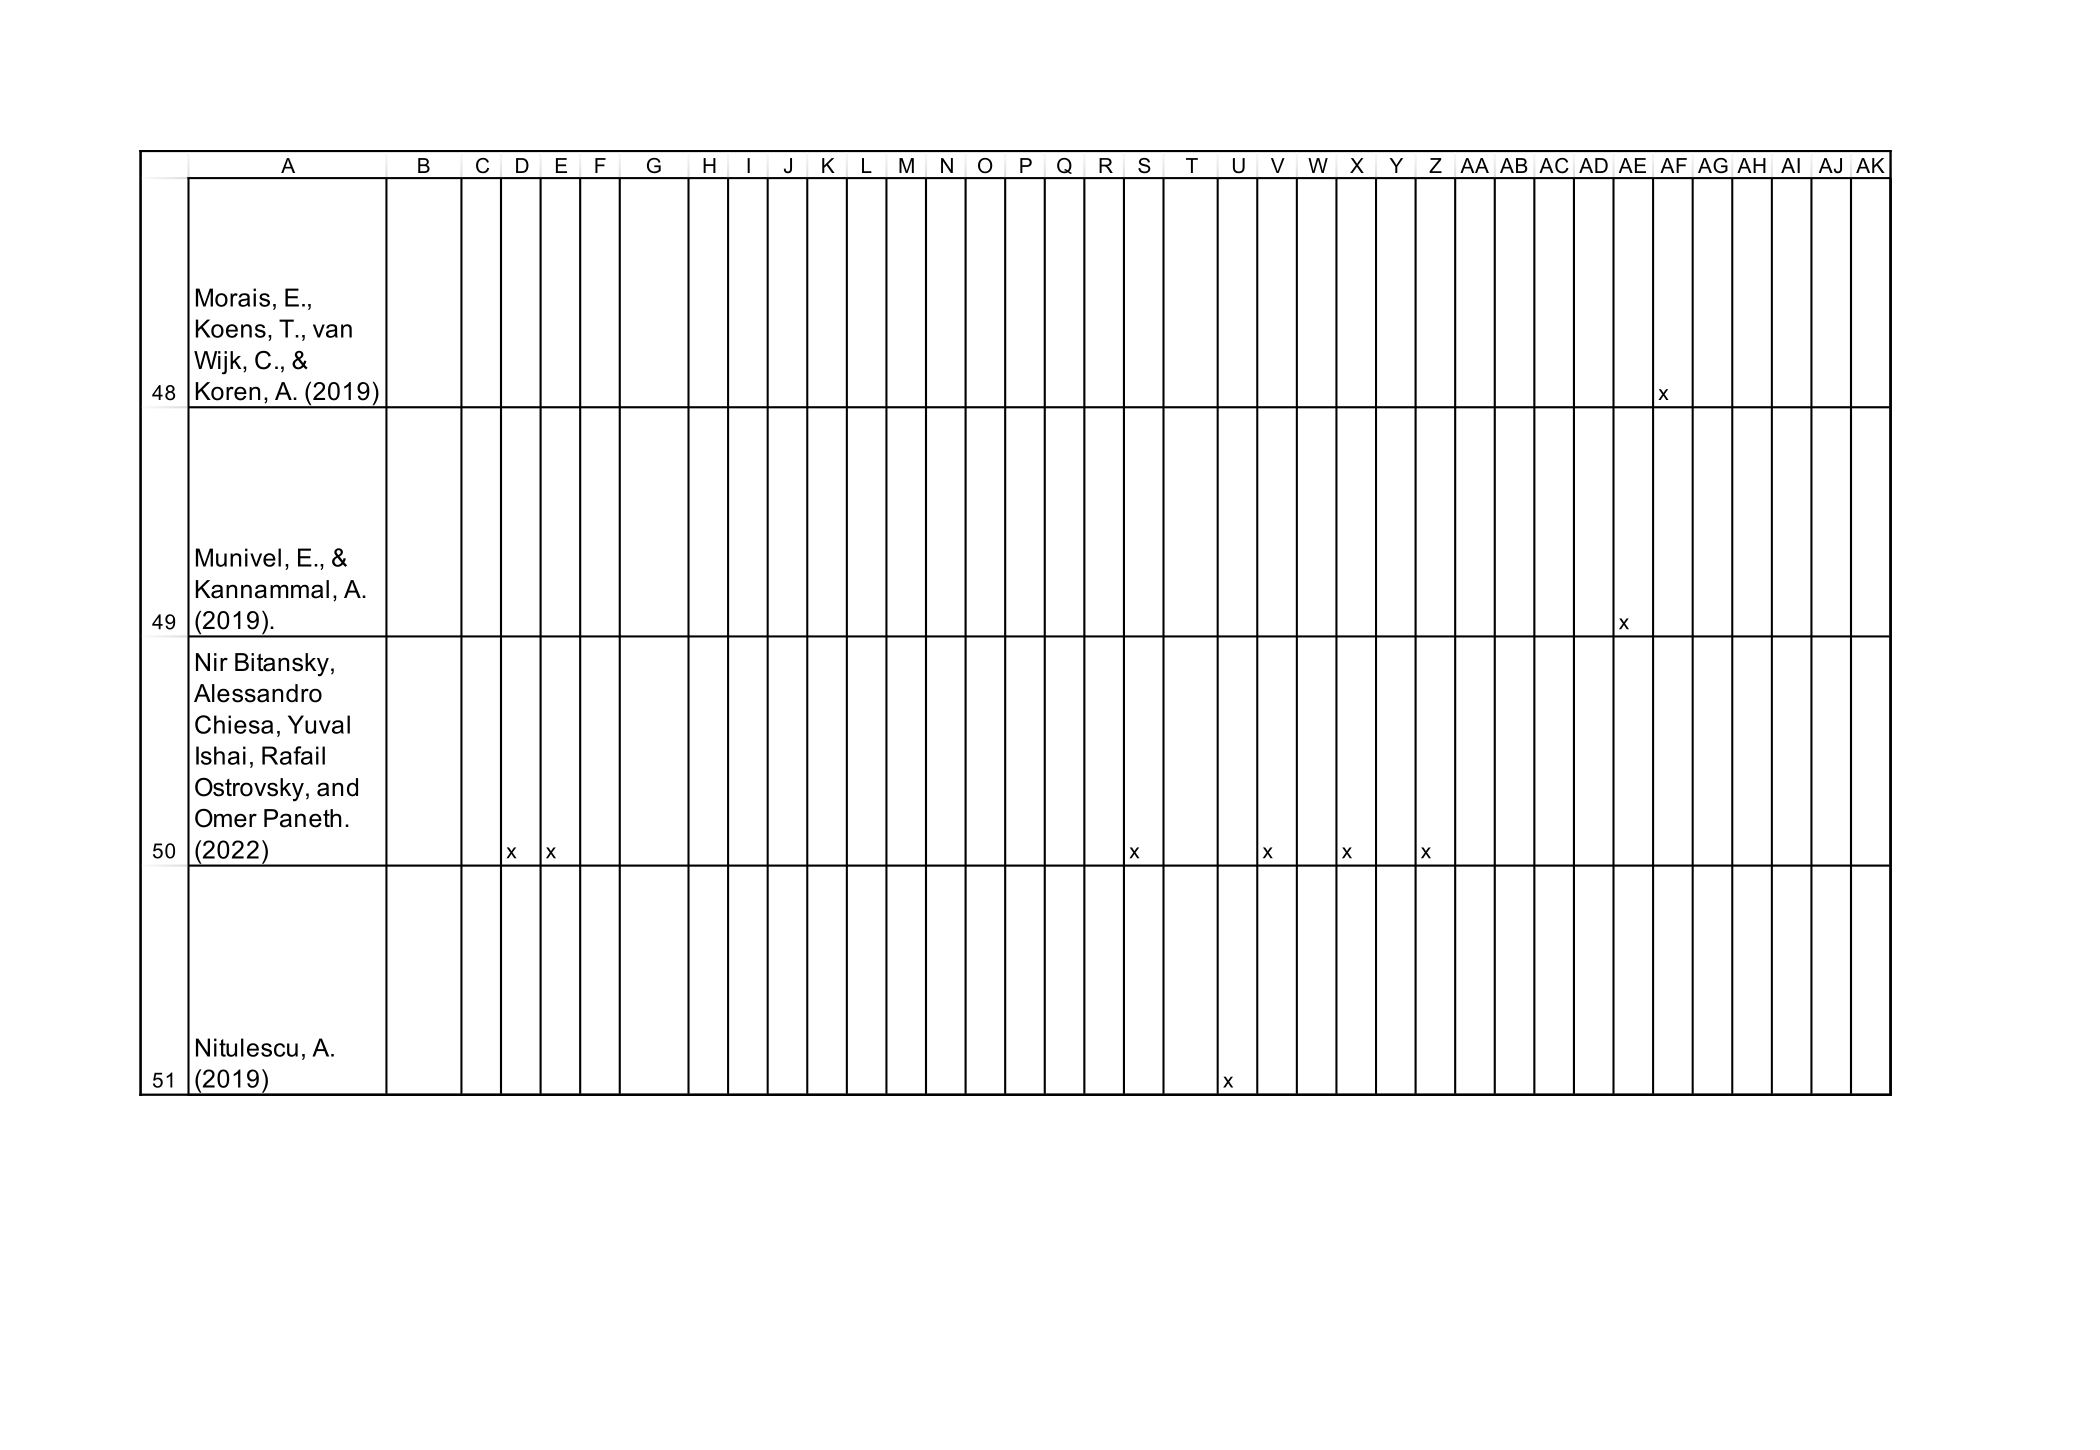
\includegraphics[width=.95\textwidth]{Pictures/concept_matrix/wos-13.png}
\end{figure}

\begin{figure}[H]
	\centering
		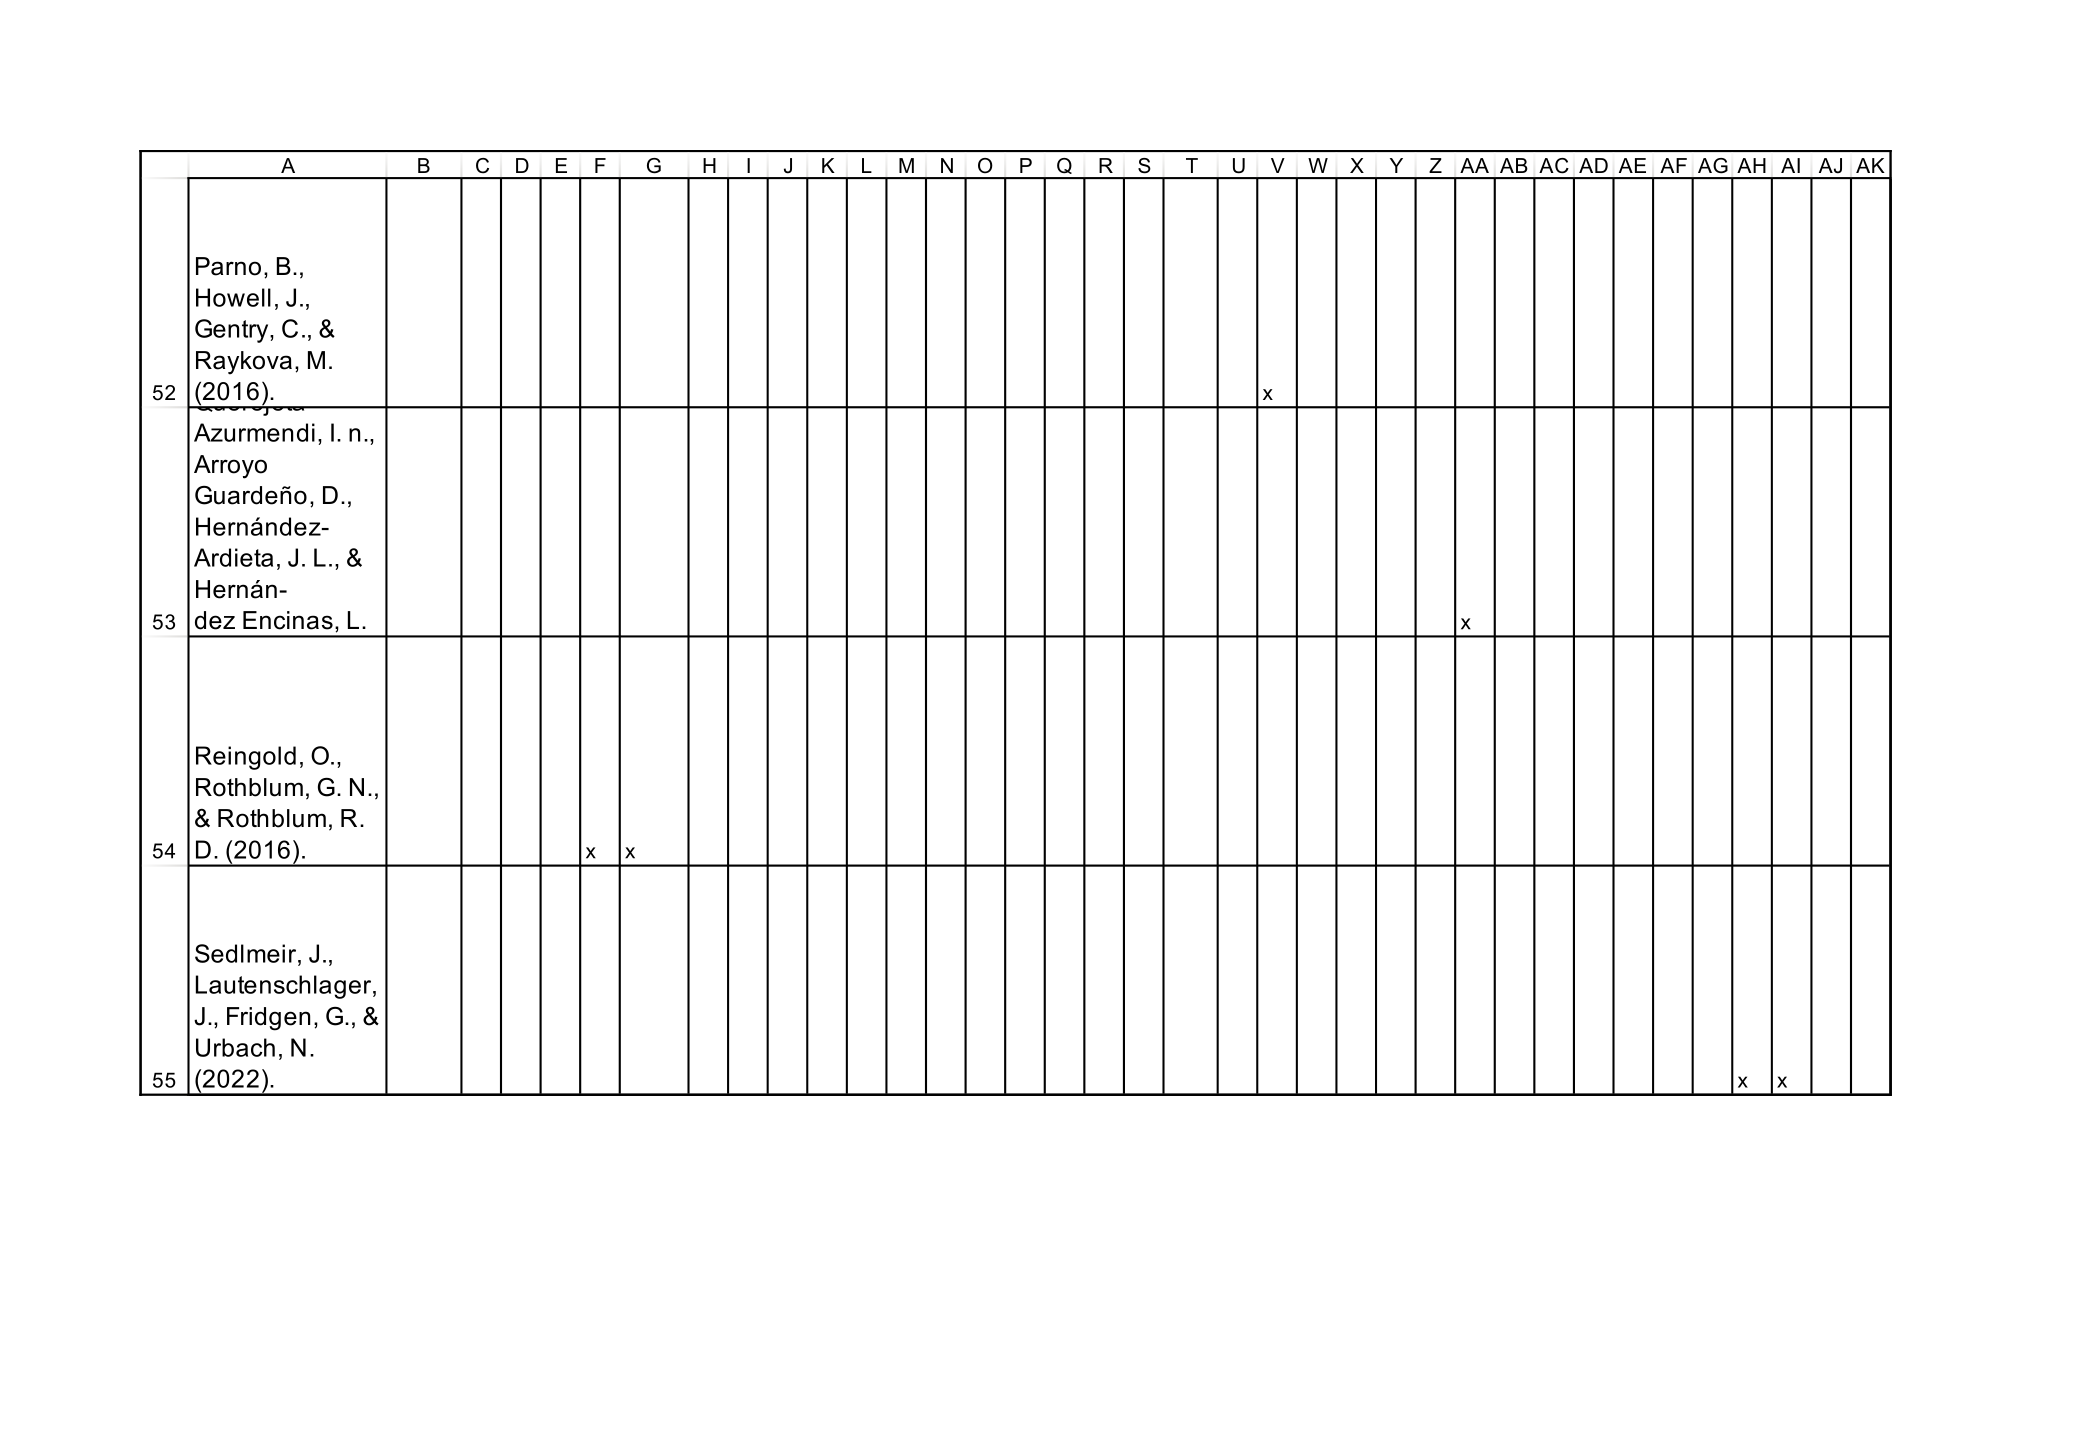
\includegraphics[width=.95\textwidth]{Pictures/concept_matrix/wos-14.png}
\end{figure}

\begin{figure}[H]
	\centering
		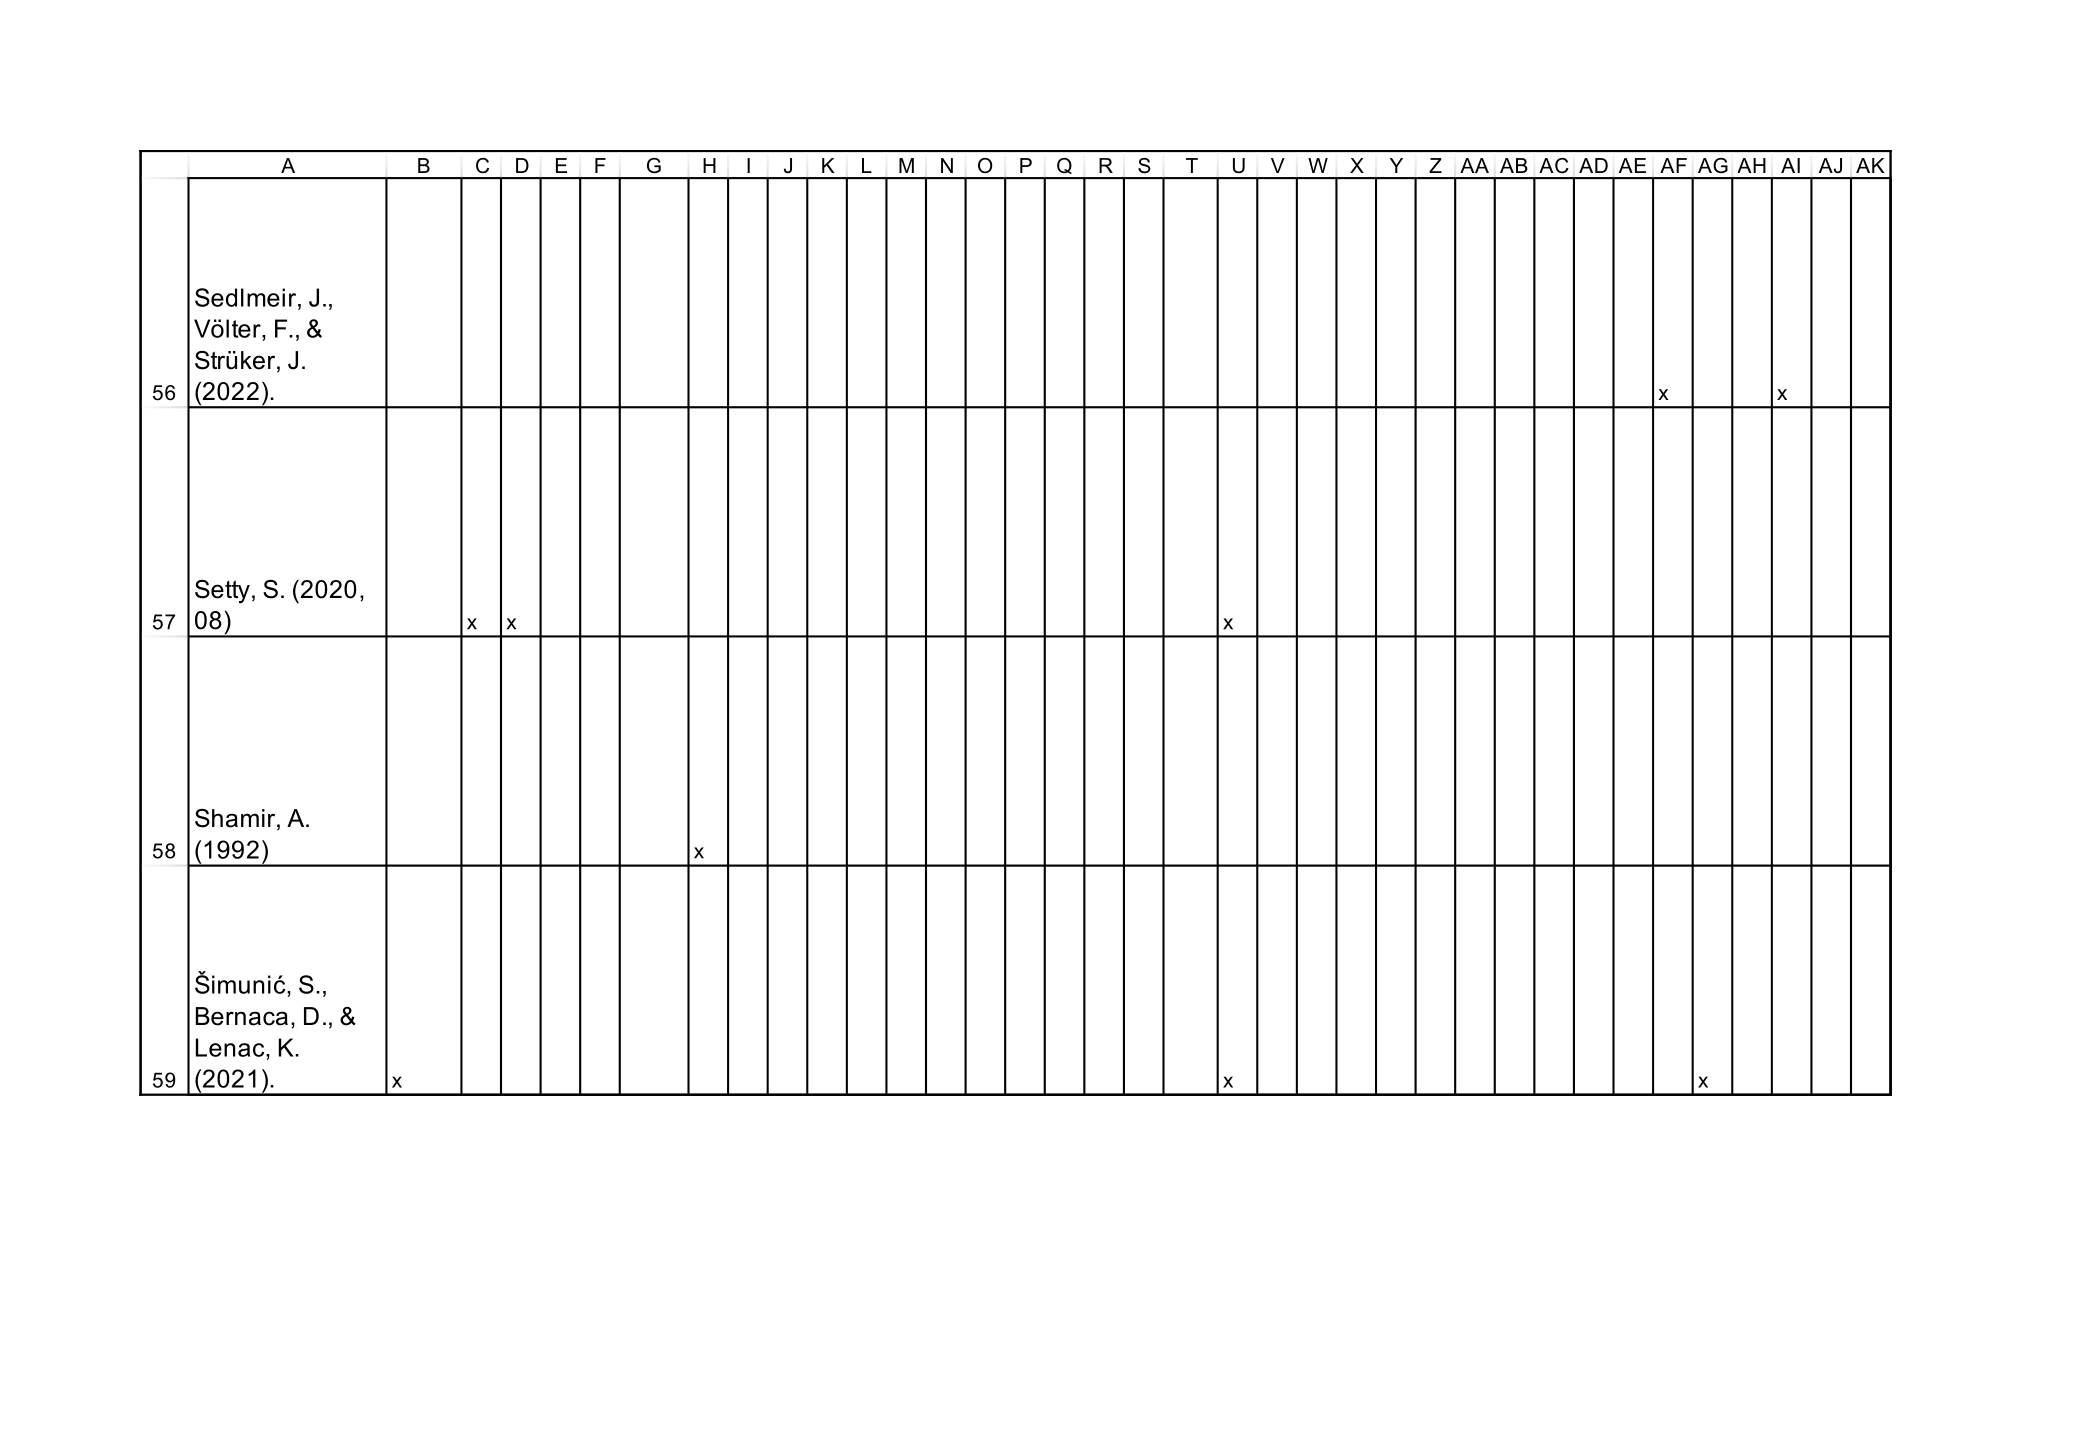
\includegraphics[width=.95\textwidth]{Pictures/concept_matrix/wos-15.png}
\end{figure}

\begin{figure}[H]
	\centering
		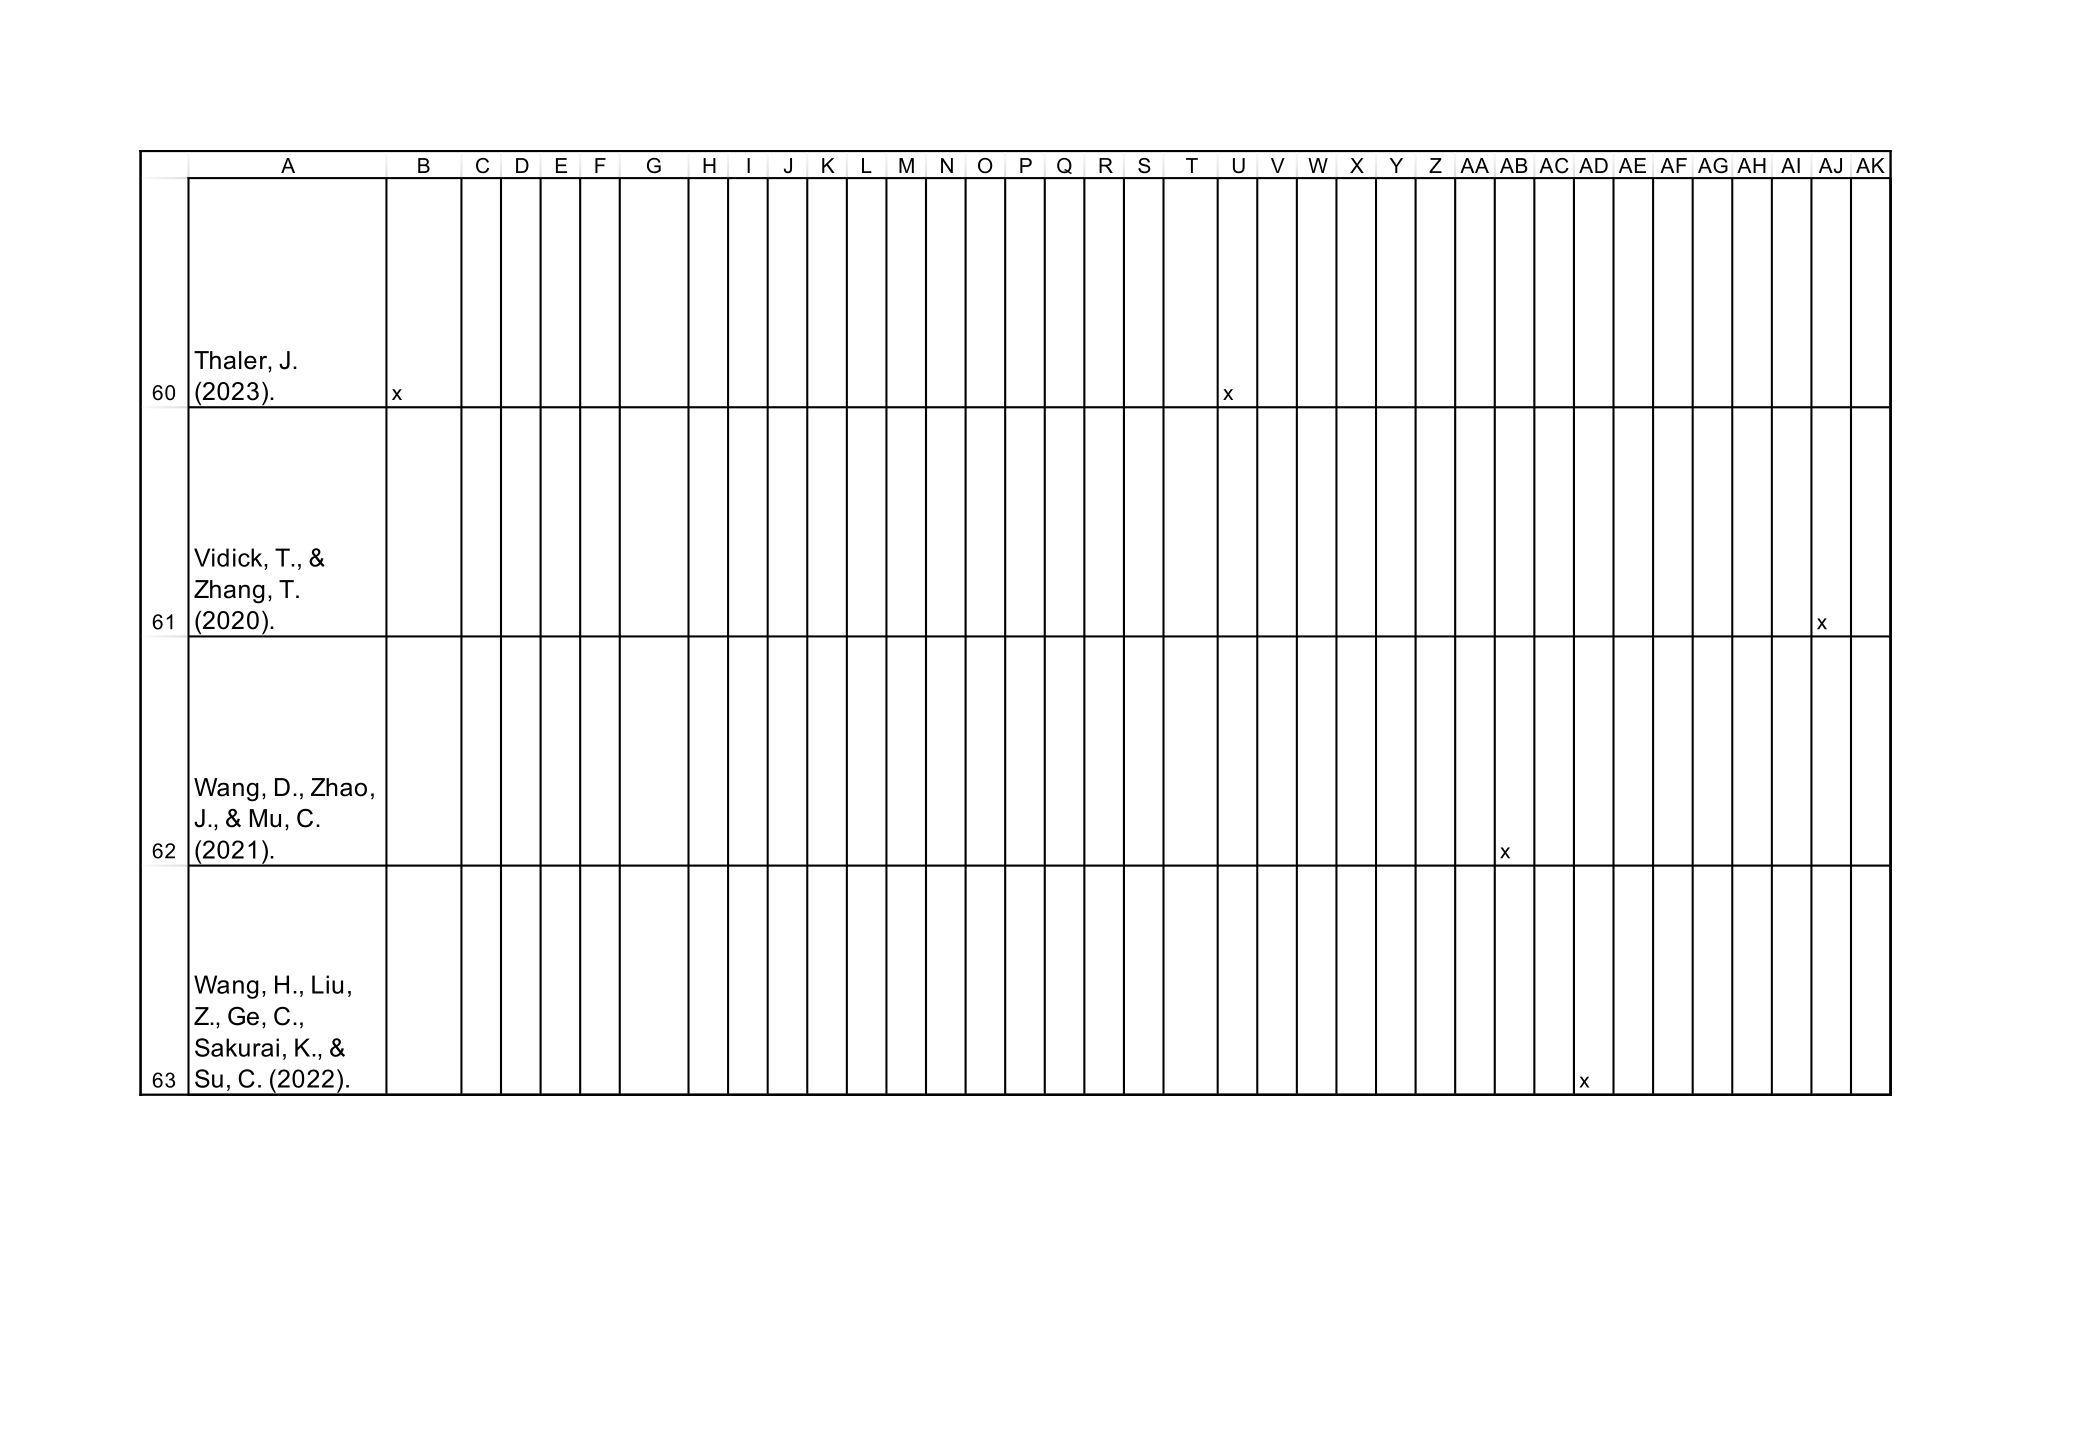
\includegraphics[width=.95\textwidth]{Pictures/concept_matrix/wos-16.png}
\end{figure}

\begin{figure}[H]
	\centering
		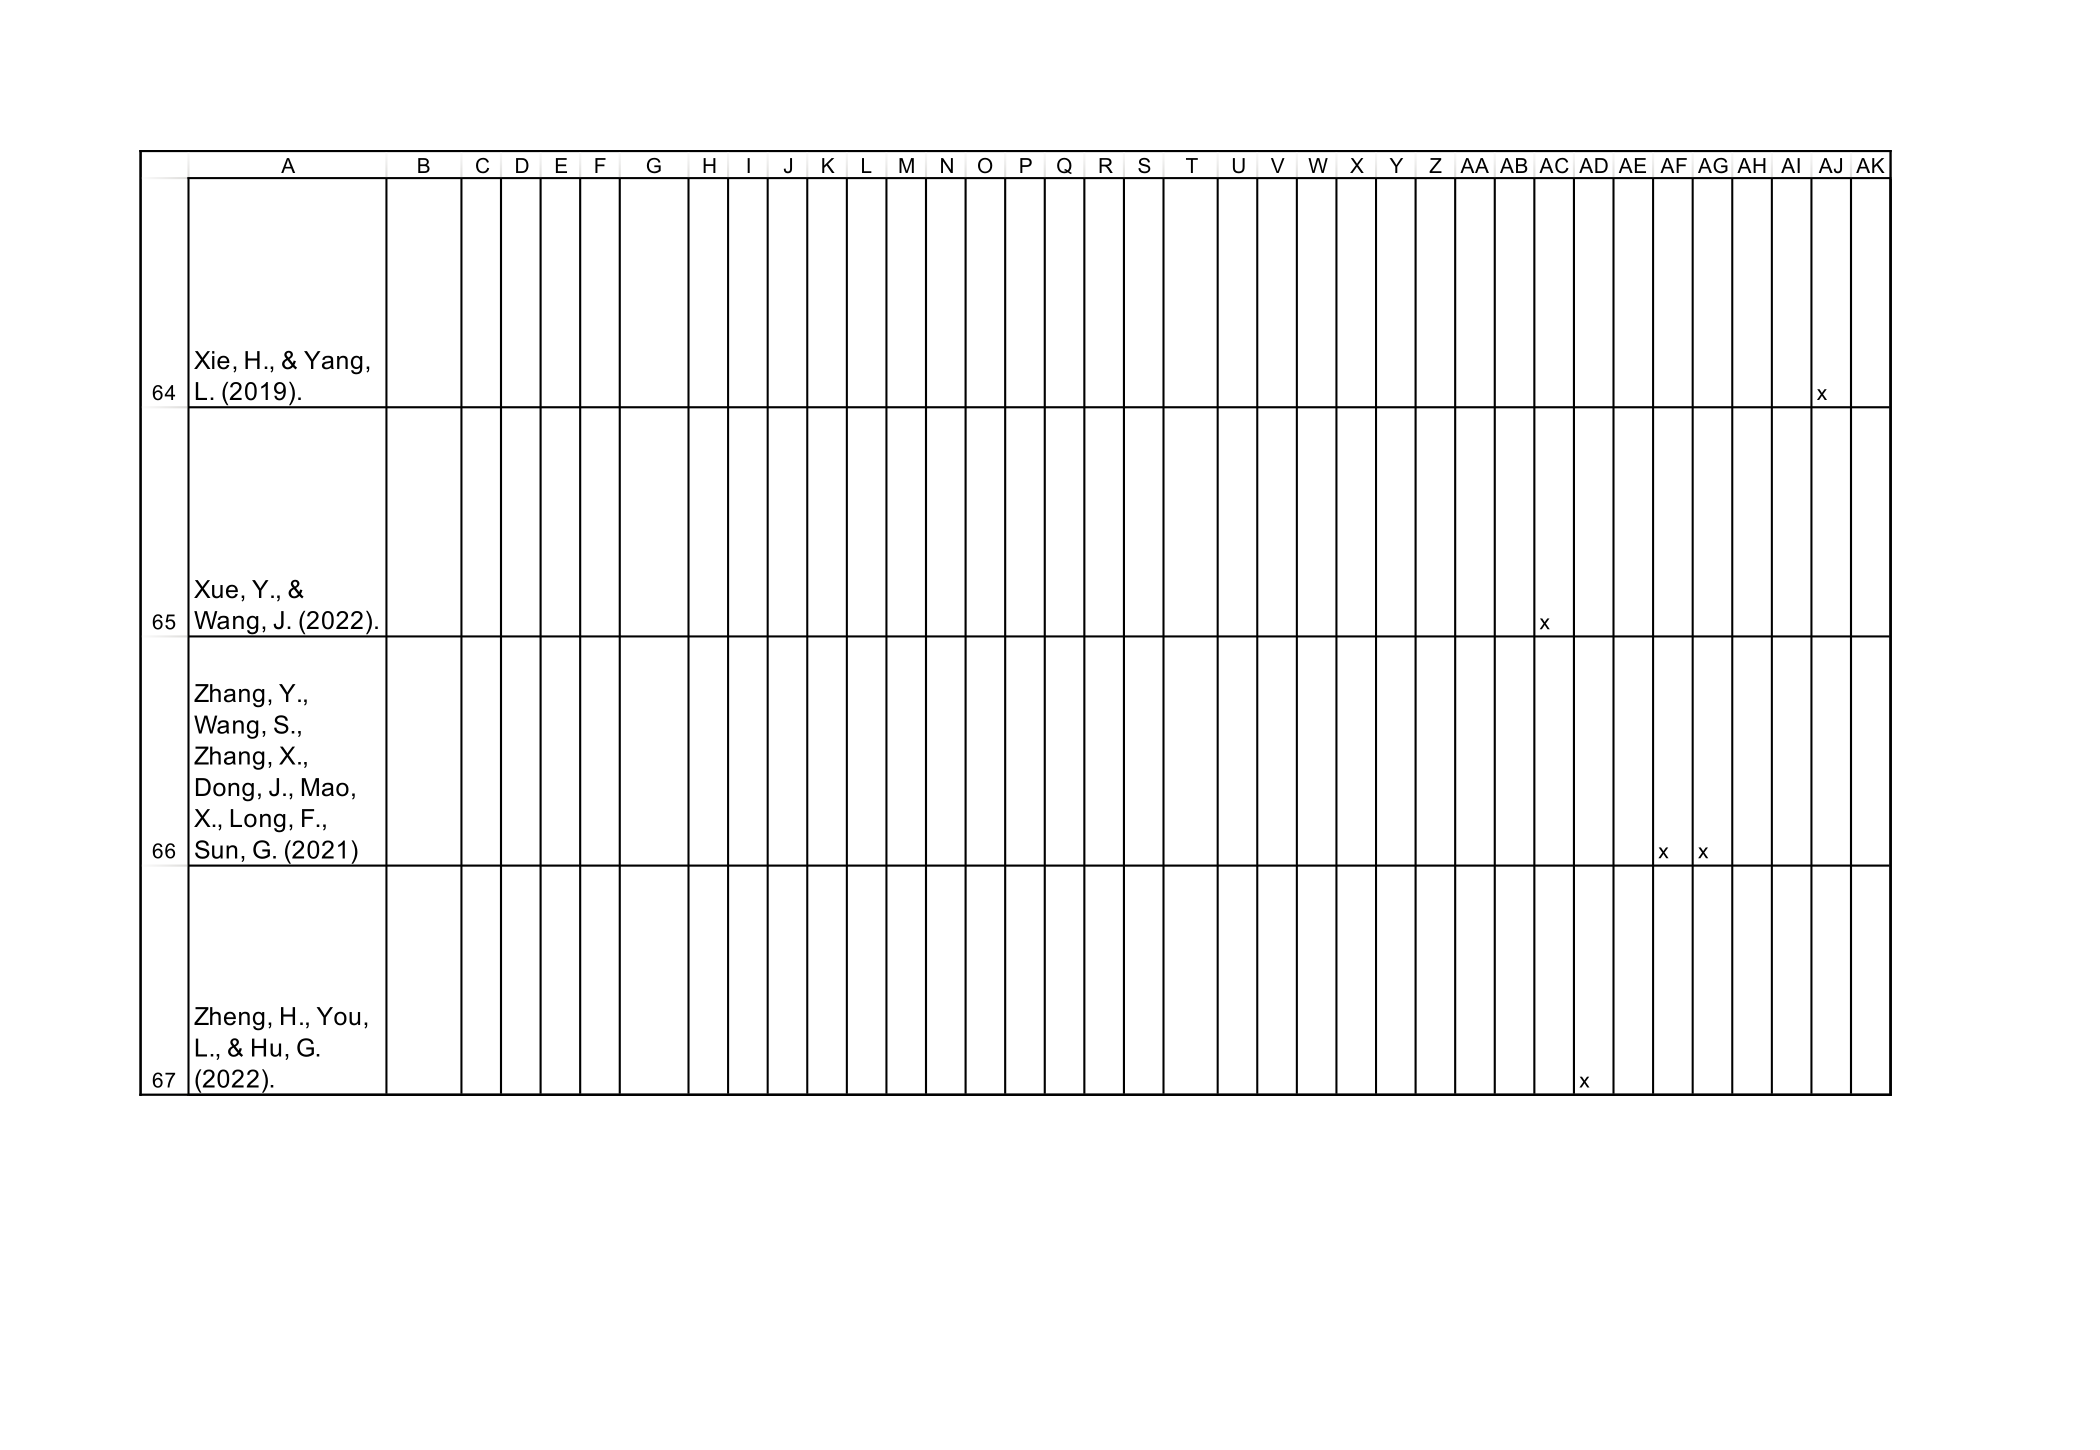
\includegraphics[width=.95\textwidth]{Pictures/concept_matrix/wos-17.png}
\end{figure}

\begin{figure}[H]
	\centering
		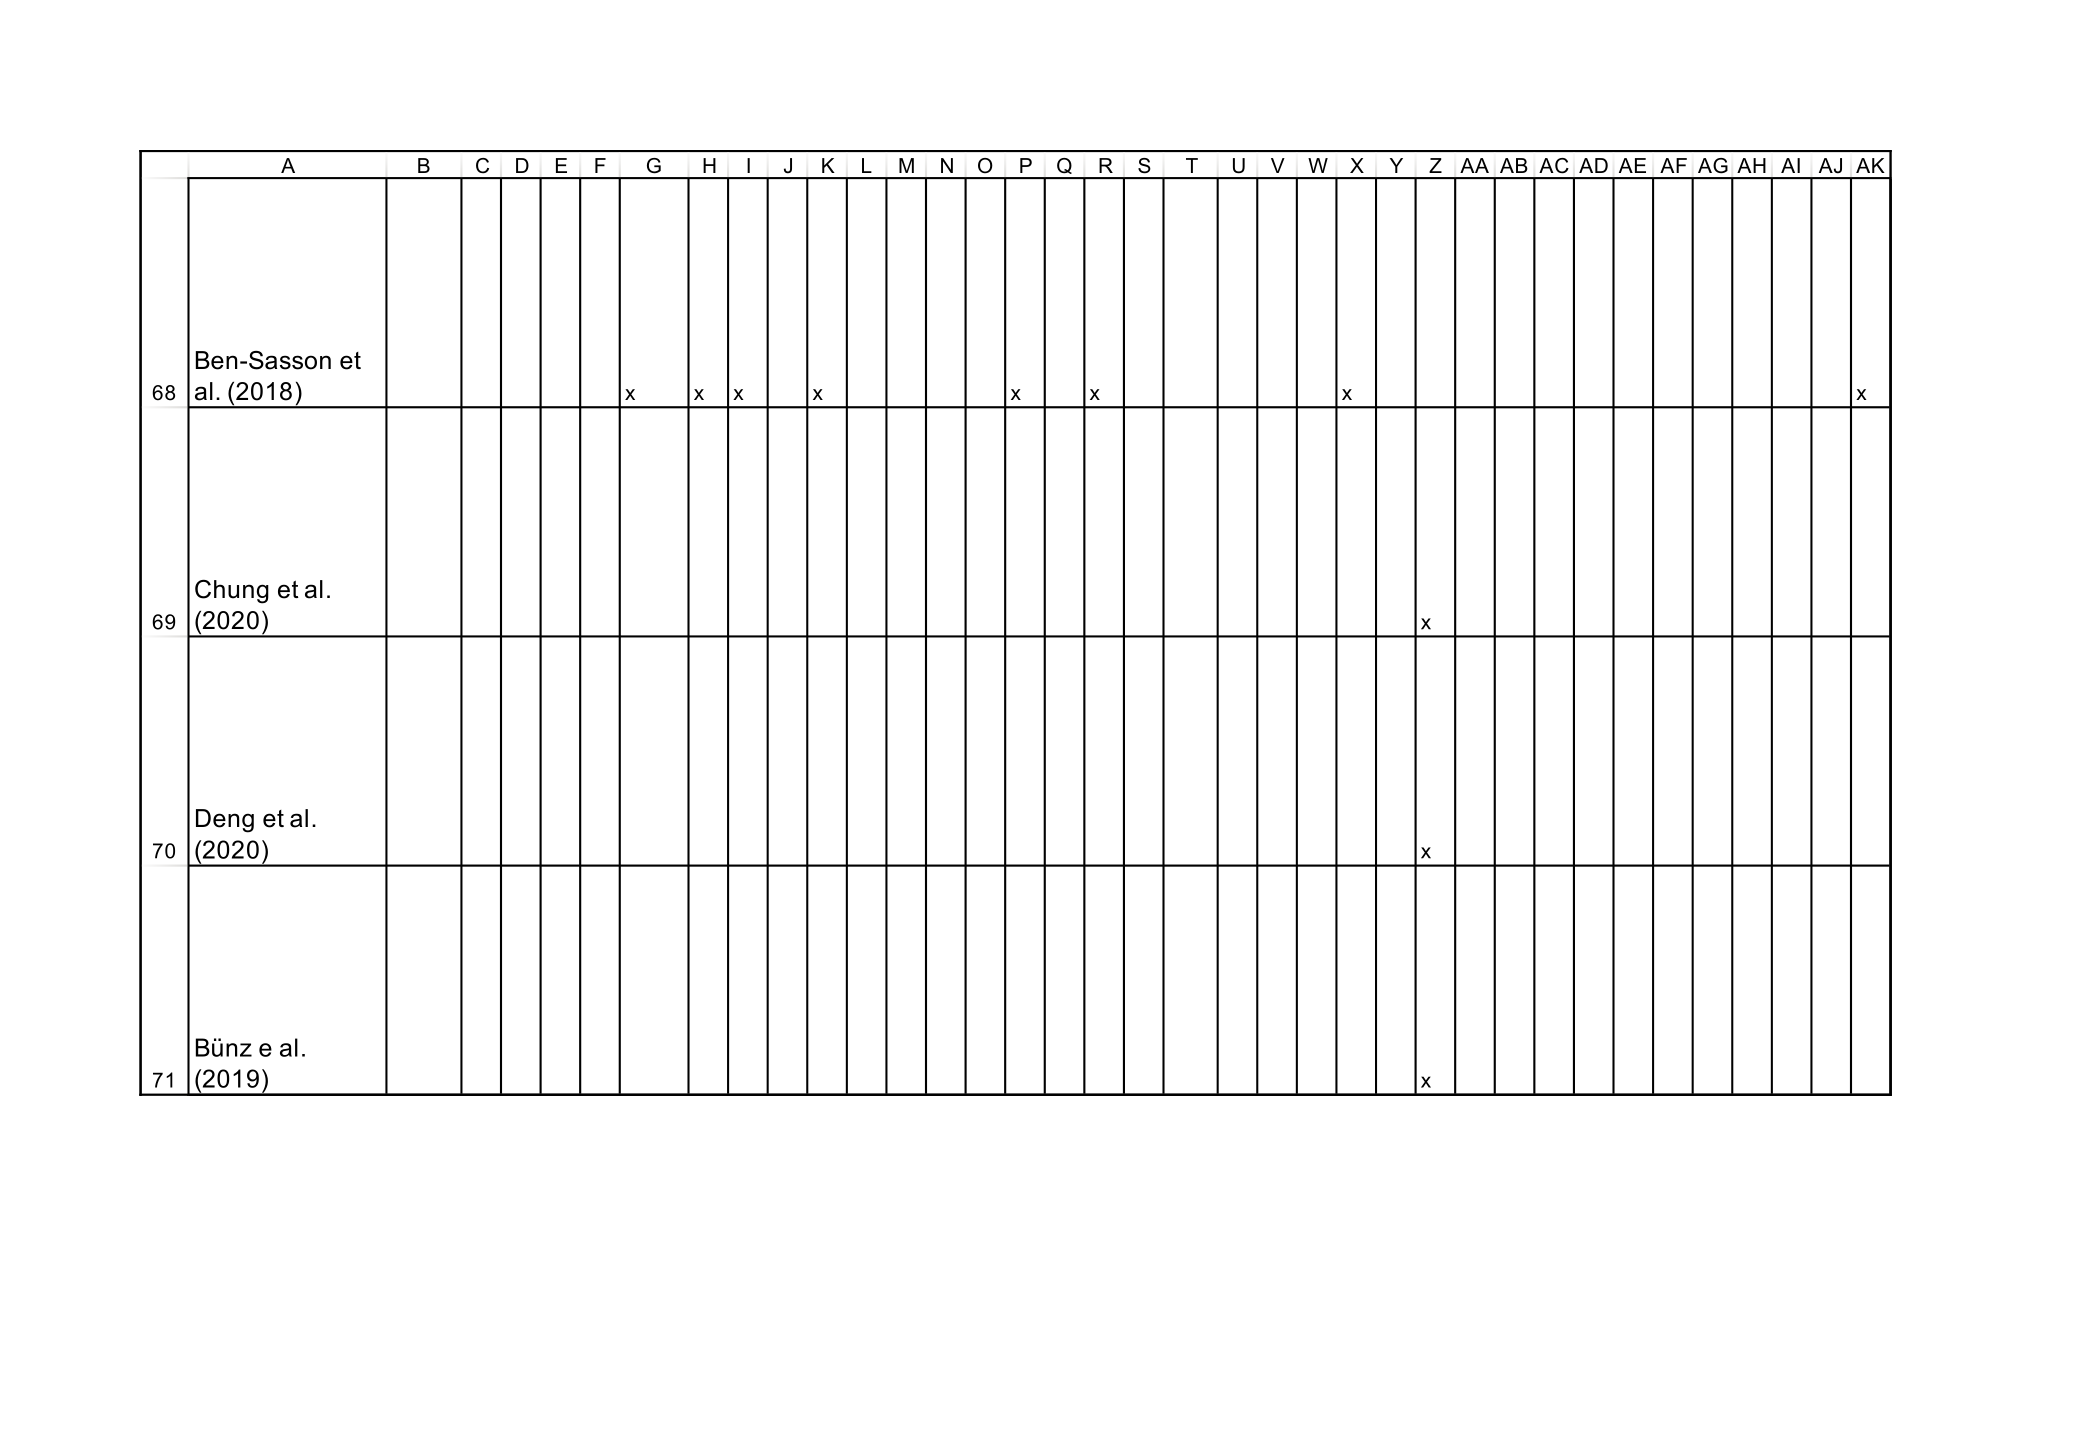
\includegraphics[width=.95\textwidth]{Pictures/concept_matrix/wos-18.png}
\end{figure}
\newpage
\subsection*{zk-DApp for MRO Attestations (Additional Screenshots)} \label{Appendix B}

\begin{figure}[H]
	\centering
		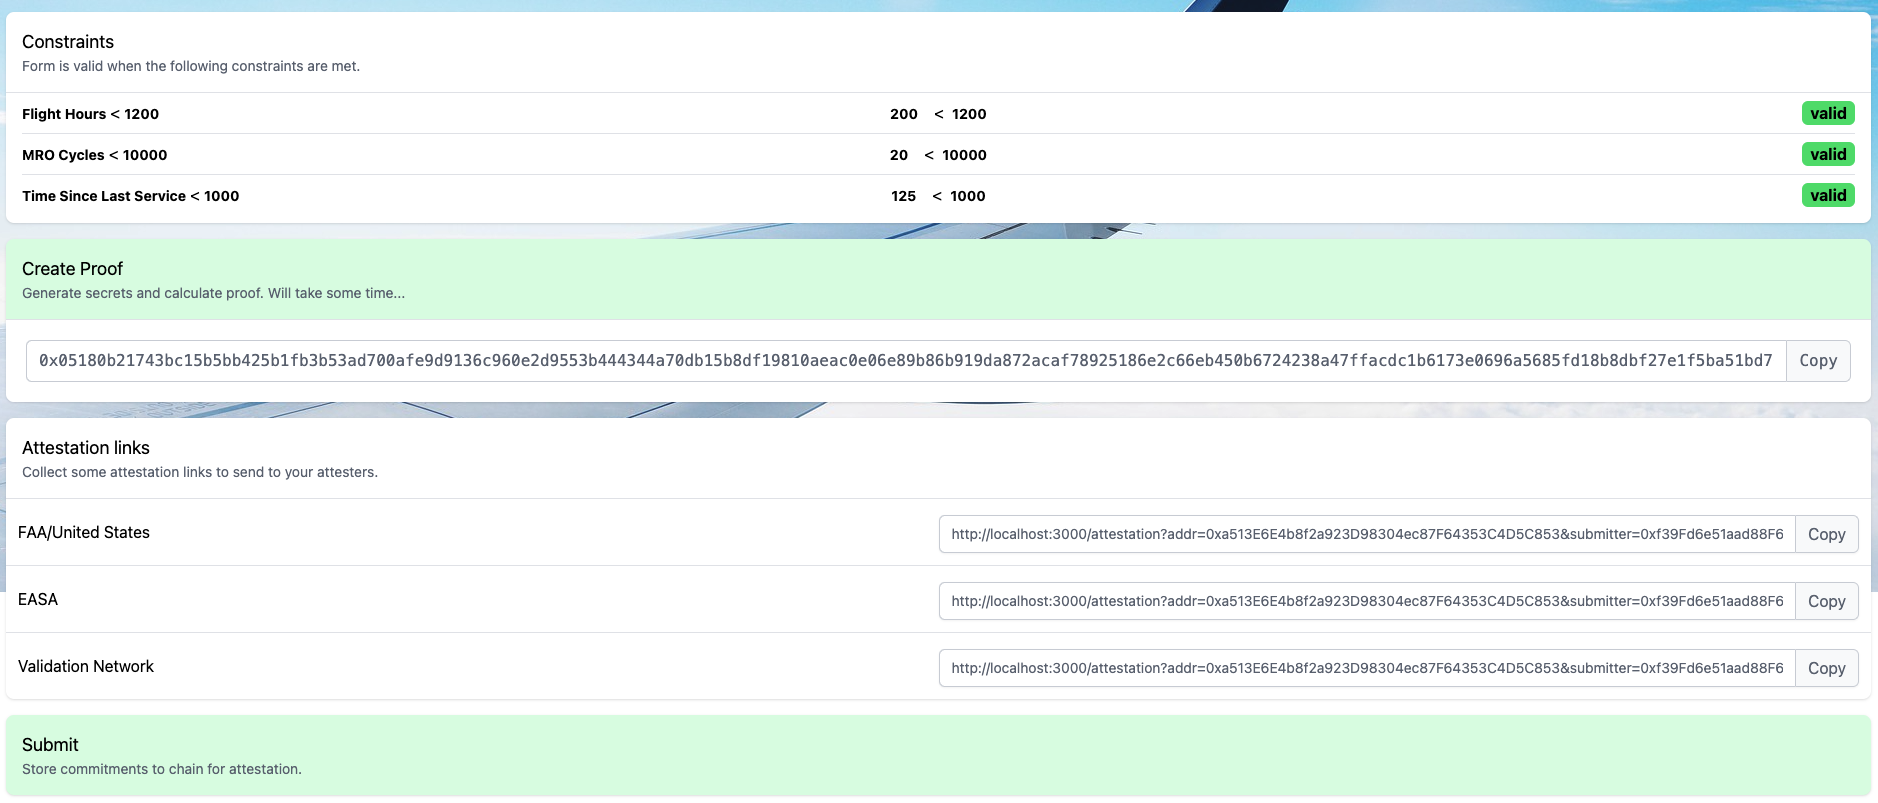
\includegraphics[width=1.0\textwidth]{Pictures/form_proof_const.png}
\end{figure}

\begin{figure}[H]
	\centering
		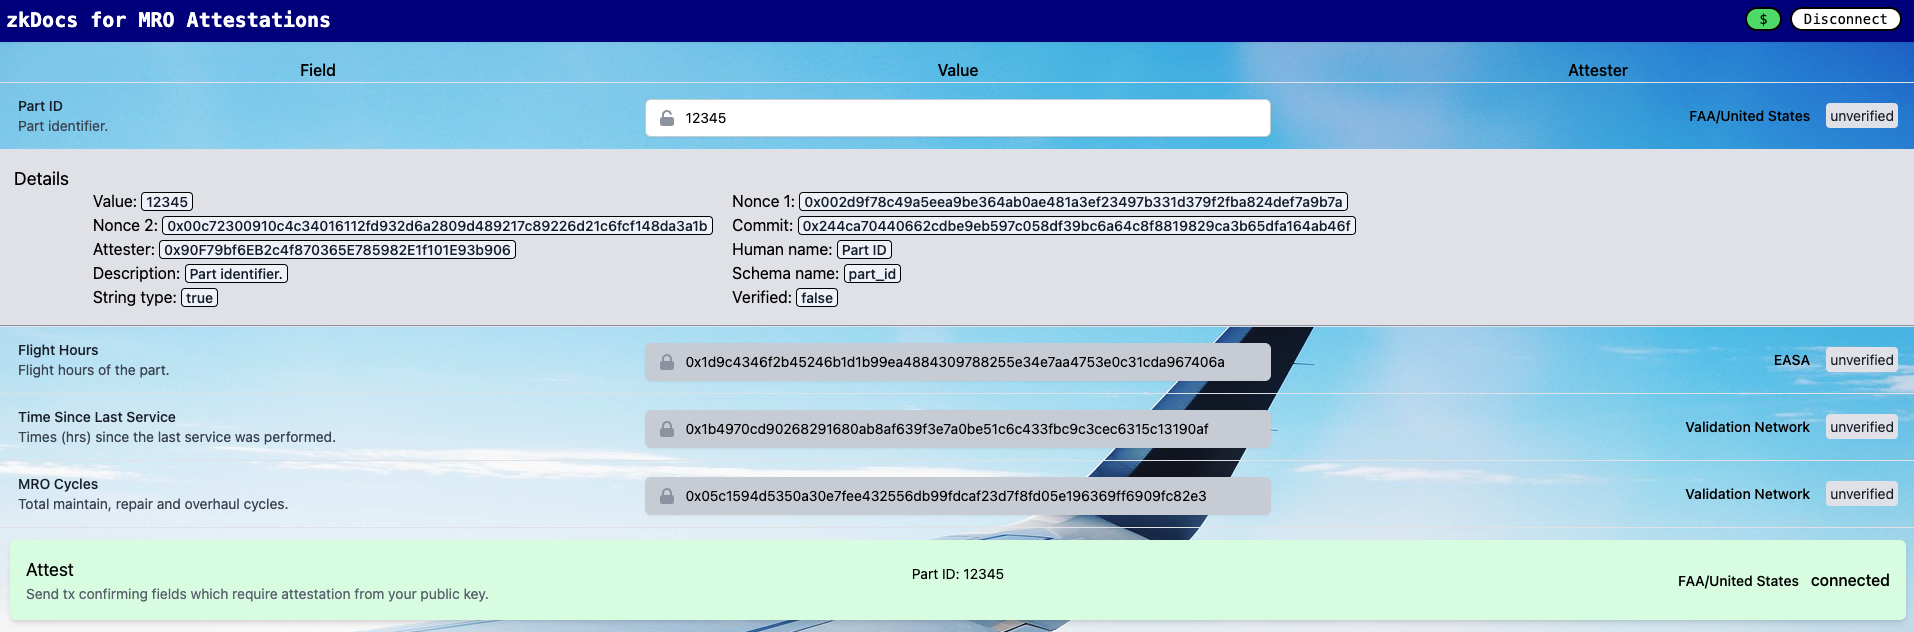
\includegraphics[width=1.0\textwidth]{Pictures/faa_attest_page.png}
\end{figure}           % Appendix
\newpage
\thispagestyle{empty}

\begin{large}

\vspace*{2cm}

\noindent
I declare that I have authored this thesis independently, that I have not used other than the declared
sources / resources, and that I have explicitly marked all material which has been quoted either
literally or by content from the used sources. 

\vspace{2cm}

\noindent
Berlin, 12 June 2023
\vspace{3cm}

\hspace*{\fill}
\begin{tabular}{l}  %% if you want centered alignment use 'c' instead of 'l'
Signature \\[1ex]
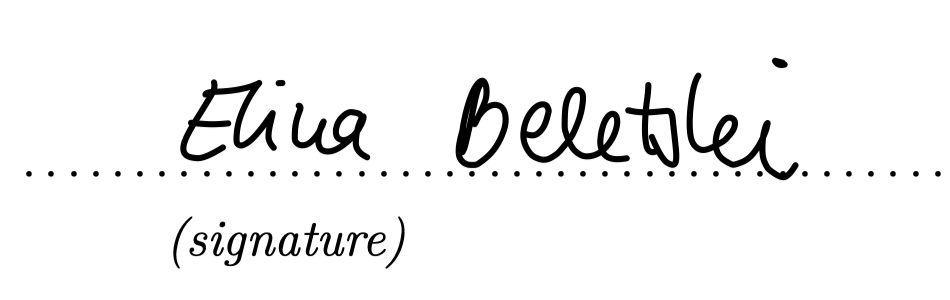
\includegraphics[scale=0.5]{Pictures/signature.png}
\end{tabular}
\end{large}
 % Eidesstattliche Erklärung (nicht bei Seminararb.)

\end{document}